\documentclass[preprint, 3p,
authoryear]{elsarticle} %review=doublespace preprint=single 5p=2 column
%%% Begin My package additions %%%%%%%%%%%%%%%%%%%

\usepackage[hyphens]{url}

  \journal{Journal of Commodity Markets} % Sets Journal name

\usepackage{graphicx}
%%%%%%%%%%%%%%%% end my additions to header

\usepackage[T1]{fontenc}
\usepackage{lmodern}
\usepackage{amssymb,amsmath}
% TODO: Currently lineno needs to be loaded after amsmath because of conflict
% https://github.com/latex-lineno/lineno/issues/5
\usepackage{lineno} % add
\usepackage{ifxetex,ifluatex}
\usepackage{fixltx2e} % provides \textsubscript
% use upquote if available, for straight quotes in verbatim environments
\IfFileExists{upquote.sty}{\usepackage{upquote}}{}
\ifnum 0\ifxetex 1\fi\ifluatex 1\fi=0 % if pdftex
  \usepackage[utf8]{inputenc}
\else % if luatex or xelatex
  \usepackage{fontspec}
  \ifxetex
    \usepackage{xltxtra,xunicode}
  \fi
  \defaultfontfeatures{Mapping=tex-text,Scale=MatchLowercase}
  \newcommand{\euro}{€}
\fi
% use microtype if available
\IfFileExists{microtype.sty}{\usepackage{microtype}}{}
\usepackage[]{natbib}
\bibliographystyle{elsarticle-harv}

\ifxetex
  \usepackage[setpagesize=false, % page size defined by xetex
              unicode=false, % unicode breaks when used with xetex
              xetex]{hyperref}
\else
  \usepackage[unicode=true]{hyperref}
\fi
\hypersetup{breaklinks=true,
            bookmarks=true,
            pdfauthor={},
            pdftitle={European Carbon Market Connectedness and Risk Contagion: A Study of Return and Volatility Dynamics Between European Union Allowances (EUAs) and Financial Markets Between 2013 and 2025 and their Potential for Portfolio Diversification},
            colorlinks=false,
            urlcolor=blue,
            linkcolor=magenta,
            pdfborder={0 0 0}}

\setcounter{secnumdepth}{5}
% Pandoc toggle for numbering sections (defaults to be off)


% tightlist command for lists without linebreak
\providecommand{\tightlist}{%
  \setlength{\itemsep}{0pt}\setlength{\parskip}{0pt}}




\usepackage{subcaption, graphicx, pdflscape, float} \graphicspath{ {./figures/} }



\begin{document}


\begin{frontmatter}

  \title{European Carbon Market Connectedness and Risk Contagion: A
Study of Return and Volatility Dynamics Between European Union
Allowances (EUAs) and Financial Markets Between 2013 and 2025 and their
Potential for Portfolio Diversification}
      \cortext[cor1]{Corresponding author}
  
  \begin{abstract}
  This paper uses Diebold-Yilmaz model to analyze the return and
  volatility connectedness between the European carbon market and the
  financial markets from the commencement of the 3rd phase of the EU
  emissions trading system in 2013 to the 4th phase until January 2025
  in order to ascertain the impact of fixed income, equity, commodities,
  and energy markets, as well as exogenous shocks and the recent reforms
  introduced under the Fit for 55 package and RePowerEU Plan. We examine
  the static and dynamic characteristics of the connectedness network
  and find that the return and volatility behavior of the European
  carbon market are primarily driven by their own fundamental factors.
  Thus it is largely independent of other financial markets except for
  coal and natural gas, and except during periods of financial stress
  where a relatively short-lived increase in the connectedness with
  other financial markets is observed. With such characteristics, EUAs
  can offer diversification benefits, especially for non-energy
  portfolios.
  \end{abstract}
    \begin{keyword}
    Carbon markets \sep emissions trading system \sep connectedness
measures \sep 
    risk diversification
  \end{keyword}
  
 \end{frontmatter}

\hypertarget{introduction}{%
\section{Introduction}\label{introduction}}

In the late 19th century the Swedish scientist Svante Arrhenius
discovered\footnote{Building on the works of Joseph Fourier and John Tyndall roughly half a century earlier \citep{corfee-morlot_global_2007}}
the link between the grenhouse gas effect, increases in carbon dioxide
(CO\(_2\)) concentrations in the atmosphere, and fossil fuel burning
\citep{corfee-morlot_global_2007, hart_scientific_1993, weart_discovery_2008}.
A century and a quarter later, in 2022, emissions worldwide have been
recorded at 57.4 gigatons of carbon dioxide equivalent (GtCO\(_2\)e),
with the energy sector accounting for a little over third of these at
20.9 GtCO\(_2\)e while industry accounting for another quarter at 14.4
GtCO\(_2\)e \citep{unep_emissions_2023}.

As one of the top polluters \citep{unep_emissions_2023}, the European
Union (EU) has established an ambitious climate objective of 55\%
reduction in greenhouse gas emissions (GHGs) by 2030 from the 1990
levels \citep[Art 4(1)]{regulation_2021_1119}. To ensure the feasibility
of this objective, the European Commission (EC) has adopted a
comprehensive suite of legislative changes under Fit for 55 package
within a broader sustainable growth strategy under the European Green
Deal \citep{delivering_2021}.

In parallel to its decarbonization efforts, the EU also launched
RePowerEU Plan in 2022, a strategic response to the energy crisis
triggered by Russia's invasion of Ukraine in that year
\citep{communication_2022}. This plan aims to reduce the EU's dependency
on Russian fossil fuels by significantly accelerating the transition to
renewable energy sources, enhancing energy efficiency, and diversifying
the EU's energy supply chains \citep[1-5]{communication_2022}.

Under Fit for 55, the EC has proposed a set of reforms to the EU
emissions trading system (EU ETS) which have duly been adopted by the
European Commission in May 2023 \citep{directive_2023_959}. The EU ETS
itself is one of the central instruments of the EU in its
decarbonization and energy transition efforts
\citep{decision_2015_1814, bai_drivers_2023}, and it currently covers
about 40\% of the EU's GHG
emissions\footnote{The coverage will likely increase in due course following the incorporation of maritime transport from 2024 and transposition of the reforms into national laws of member states by 30 June 2024 \citep{directive_2023_959}}
\citep{eu_ets}. Under this mechanism a European Emission Allowance (EUA)
is a permit granting the right to emit one ton of CO2 which can then be
traded \citep{directive_2003_87}.

The EU ETS has evolved over four phases. The first phase, covering the
period from 2005 to 2007, has essentially established the market
mechanism underpinning the EU ETS \citep[Art. 11(1)]{directive_2003_87}.
The second phase, covering the five-year period from 1st of January
2008, has imposed a more stringent cap on the Union-wide total EUAs but
the mechanism still ended up with surplus of allowances largely due to
the 2008 recession \citep{ellerman_eu_2014, bel_emission_2015}. With the
commencement of the third phase on 1 January 2013, there has been a
shift from national allocation
plans\footnote{During the phases I and II of the EU emissions trading system (EU-ETS), each EU country decided on the allocation of their emission allowances. \citep[Art. 11]{directive_2003_87}}
to an EU-wide cap in the total number of
allowances\footnote{The total number of annual allowances also decrease by a linear factor of 1.74 percent. To address the surplus allowances that have been accumulating since Phase II, a new market stability reserve (MSR) has additionally been introduced that acts as a repository for excess portions of auctionable allowances and replenishes the market if allowances in circulation are fewer than 400 million \citep{decision_2015_1814, simoes_revision_2022}}
\citep[Art. 1]{directive_2009_29}. The fourth and current phase that
started in 2021, and will continue until 2030, has further reduced the
EU-wide allowance cap with more stringent rules for free
allocation\footnote{It also increased the annual reduction factor to 2.2 percent and earmarked a portion of MSR for innovation support.}
\citep{directive_2018_410}. In parallel, the Fit for 55 package has,
among other initiatives, extended the scope of the ETS to include
emissions from shipping and has accelerated the reduction of both the
free allocations and the total allowances within Phase
IV\footnote{This was done by increasing the linear reduction factor from 2.2 percent to 4.2 percent starting in 2024.}
\citep{directive_2023_959}.

The effectiveness of the EU ETS in decarbonizing and facilitating the
energy transition depends on several factors
\citep{backe_exploring_2023, de_cara_marginal_2011, marin_impact_2018, scheelhaase_options_2021}.
Among these factors, the price of EUAs plays a critical role
\citep{pietzcker_tightening_2021, quemin_raising_2022, lovcha_determinants_2022}.
Higher EUA prices have the potential to drive significant
transformations across multiple sectors, encouraging firms to innovate
and reduce emissions \citep{pietzcker_tightening_2021, recka_2015}. Such
realization of higher EUA prices can be aided by increased participation
of financial institutions which can promote liquidity, price discovery,
transparency, and improved market efficiency
\citep{bohl_impact_2023, corgnet_information_2021}. This in turn
depends, among other factors, on the price volatility
\citep{acworth_emissions_2017, laing_assessing_2013}, on policy
uncertainty,
\citep{raza_forecasting_2023, fang_effect_2018, zhu_does_2020, wang_commodity_2015},
on market stress due to geopolitical and other exogenous shocks such as
Covid-19
\citep{deng_dynamic_2024, yang_time-varying_2022, tiwari_quantile_2022, babar_returns_2024},
and on financial stress
\citep{bakas_impact_2018, ding_time-varying_2021} which can raise
uncertainty and restrain investment into carbon-reducing technologies.

This study, therefore, analyzes, via return and volatility connectedness
of EUAs with other financial markets, the extent to which EU Fit for 55
and RePowerEU as potential policy shocks, and market stress due to
Russian-Ukrainian War and Covid-19 impact the degree of integration of
EUAs with other asset classes with a broader view to assess potential
diversification benefits EUAs may offer. If present, such
diversification benefits can consequently incentivize increased
participation by financial institutions and help the EU's efforts in
decarbonization and transitioning into renewables. Accordingly, this
study contributes to the literature on energy and sustainable finance as
well as on risk management in three complementary ways. First, carbon is
treated as an independent asset class whereas previous works largely
examine the issue within an energy context. To the best of our
knowledge, this is the first time it is treated as such while examining
the impact of the changes emerging from the potential policy shocks of
Fit for 55 package and RePowerEU. Within this context, this study
uniquely considers return and volatility spillovers within a broader
range of markets, ranging from fixed income and European and US equities
to commodities. Second, while the existing literature largely considers
Phase III of EU ETS, this study also incorporates Phase IV to date,
providing a more comprehensive analysis of the recent changes. Third,
market stress periods -- such as Covid-19 and the Russian-Ukrainian War
-- are uniquely considered in analyzing the changes in EU ETS
connectedness and its integration with other asset classes over time.

Three key results emerge from this study. First, we find that EUAs show
stronger connection with other financial markets almost exclusively
during periods of financial crises. However, aside from connectedness
with coal and natural gas markets, these connections tend to be
short-lived, and EUAs generally remain independent. Second, our results
indicate that the European carbon market tend to be a net receiver of
return and volatility spillovers, suggesting that external factors
influence this market more than carbon-specific factors influence other
markets. Third, it appears that to date the reforms introduced by the
Fit for 55 package, RePowerEU, and Phase IV may not have exerted as
strong an impact as market stresses, although it seems that their impact
may have a longer duration.

The rest of the paper is as follows. The next section provides a
literature review of the related studies. Section \ref{data_section}
describes the data, and Section \ref{method} specifies the methodology.
Section \ref{results} presents the main empirical findings and
discussion, and Section \ref{conclusion} provides our concluding remarks
and implications.

\hypertarget{literature-review}{%
\section{Literature Review}\label{literature-review}}

Since the EU ETS has come into force, empirical literature on carbon
trading mechanisms has mainly focused on its impact on the economy, its
price dynamics, and its relationship with various markets along with its
hedging benefits \citep{demiralay_carbon_2022, dai_impact_2022}.

With respect to its impact on the economy, emissions trading can help
reduce the abatement costs and dampen the negative impact of emission
reductions on GDP \citep{wu_achieving_2016, lin_impacts_2019}, although
some of the carbon reduction gains may decline overtime due to
macroeconomic carbon rebound effect \citep{bolat_is_2023}. Nevertheless,
its impact on the economy mainly has a sectoral perspective. Within that
perspective, the predominant focus is on its strong impact on the energy
industry
\citep{delarue_simulating_2007, kara_impacts_2008, zachmann_first_2008, kirat_impact_2011, bonenti_evaluating_2013, hobbie_windfall_2019, hanif_nonlinear_2021, dai_impact_2022},
and, to a lesser extent, on its negligible impact on the aviation,
cement, steel, and aluminum sectors
\citep{VANASSELT2007497, zhang_overview_2010, oberndorfer_costs_2007, efthymiou_eu_2019}.

With respect to price dynamics, ability to accurately forecast carbon
prices are important in enabling decisions on emissions and transition
tradeoffs
\citep{wang_novel_2021, zhang_forecasting_2024, chen_multiscale_2024}.
To that end, while some have considered the role of attention in carbon
pricing
\citep{zheng_relationship_2022, gong_climate_2023, zhang_forecasting_2024},
some have used value-at-risk-forecasting, ARIMA, GARCH and its
modifications including, among others, Markov switching GARCH,
fractionality integrated GARCH, switching transition regression
exponential GARCH, and AR-GARCH to capture volatility, skewness, and
excess kurtosis
\citep{paolella_econometric_2008, benz_modeling_2009, arouri_nonlinearities_2012, byun_forecasting_2013, garcia-martos_modelling_2013, huang_hybrid_2021},
and some have used various decomposition and artificial intelligence
techniques to improve the forecasting ability
\citep{QIN2024131410, wang_novel_2021, chen_multiscale_2024}.

Yet others have looked at the impact of policy uncertainties on the
volatility of carbon markets. \citet{dong_extreme_2024} have found that
market risk spillovers are exacerbated by uncertainty with respect to
climate and trade policies leading to increased volatility in energy
markets in China. This to an extent confirms the broader causal
relationship between climate policy uncertainty and `traditional' energy
markets \citep{REN2023113058} where indexation of climate policy
uncertainty \citep{gavriilidis_measuring_2021} -- which itself was based
on economic policy uncertainty index developed
\citet{baker_measuring_2016} - is utilized. Similarly,
\citet{dai_impact_2022} uses both European economic policy uncertainty
index - also constructed by \citet{baker_measuring_2016} - as well as a
proxy for a similar global uncertainty index and demonstrate that both
uncertainties impact the long-term volatility of European carbon spot
return, though the effect is larger for the global policy uncertainty.
They argue that this may be due to European companies adjusting their
demand for EU ETS based on revised expectations in response to global
economic environment. What is evident is that it is a challenge to
forecast carbon prices since they are nonstationary and show
nonlinearity, and it is likely that the information shocks transmit
between different markets
\citep{chen_multiscale_2024, feng_carbon_2011, lutz_nonlinearity_2013, segnon_modeling_2017}.

In that respect, there appears to be a positive relationship, albeit in
varying degrees, between carbon markets on the one hand and equities,
oil, natural gas, coal, and electricity prices on the other
\citep{ji_information_2018, zhang_dynamic_2016, mansanet-bataller_co_2007, alberola_price_2008, keppler_causalities_2010, bredin_emerging_2011, chevallier_evaluating_2011, creti_carbon_2012, aatola_price_2013}.
However, with the changes introduced in each of the subsequent phases
such impacts became harder to establish
\citep{wu_market-linkage_2020, arouri_nonlinearities_2012}.
Nevertheless, there is likely a stronger relationship between carbon and
energy assets compared to financial assets for the duration of Phase II
and most of Phase III, which, for a non-energy portfolio, may provide
some diversification benefits
\citep{lovcha_determinants_2022, tan_how_2020, yang_idiosyncratic_2022}.
Moreover, interconnectedness of the carbon with other markets evolves
overtime and has increased with financial markets in recent years
\citep{dong_risk_2024, jimenez-rodriguez_what_2019, tan_how_2020}.
Concerning the integration of EUAs into portfolios, it seems to be the
case that incorporating a portion of carbon into stock portfolio
enhances the risk-adjusted performance of the portfolio
\citep{demiralay_carbon_2022}.

Even though many recent studies have offered some approaches to
understanding the linkage of EUAs with energy and other specific
markets, this study aims to expand that understanding further by
examining the interlinkages with the equity, fixed income, energy, and
non-energy commodity markets, and by including the data that captures
Phase IV of EU-ETS to date with a view to ascertain the impacts of Fit
for 55 reforms and the RePowerEU initiative as well as the exogenous
shocks such as COVID-19 and the Russia-Ukraine war to those linkages.
The changes introduced under Fit for 55 and RePowerEU as well as the
expansion under Phase IV could be viewed as a policy uncertainty, or
shock. If so, volatility connectedness of EU-ETS ought to exhibit
patterns that are in alignment with the previous findings of the impacts
of policy shocks. Similarly, by examining the impacts of Covid-19 and
Russia-Ukraine war we can compare the magnitude of the impacts of the
policy shocks to exogenous shocks. This understanding could benefit
investors with portfolio diversification benefits and better manage
their risks and help policy makers recognize the carbon market
volatility connectedness in policy formulation. To this end, we utilize
the following data.

\hypertarget{data}{%
\section{\texorpdfstring{Data \label{data_section}}{Data }}\label{data}}

We obtain daily price data for EUAs and other financial markets from
Bloomberg LP and Refinitiv, covering the period from January 2, 2013, to
January 9, 2025. This time frame, as shown in Figure \ref{fig:EUAprice},
encompasses Phases III and, to the extent possible, Phase IV of the
European Union Emissions Trading System (EU ETS), including the reforms
introduced under Fit for 55 package and RePowerEU. This timeframe also
captures macroeconomic events such as the 2016 Brexit referendum, the
Covid-19 pandemic, and the escalation of the Russian-Ukrainian conflict,
ensuring the data reflects diverse market regimes that includes periods
of low and high volatility, enhancing the dataset's ability to capture
dynamic interrelationships.

\begin{figure}[ht]
\caption{Europe Emission Trading System Phases and European Union Allowances (EUA) Prices}
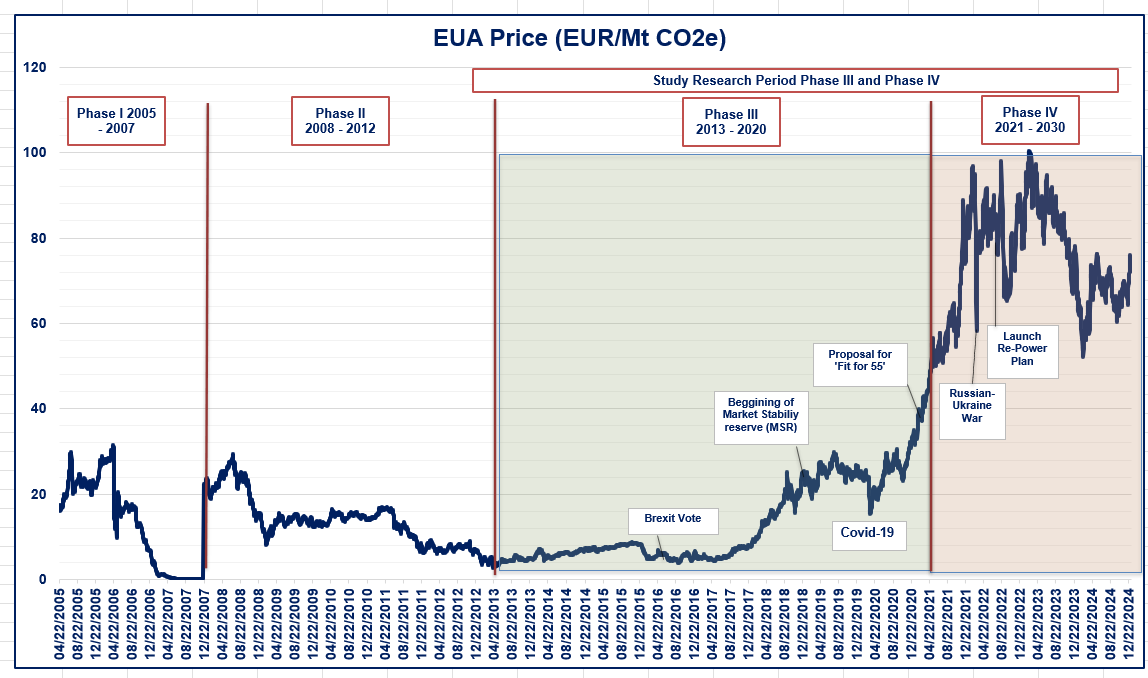
\includegraphics[width = \textwidth]{1EUAPrice}
\label{fig:EUAprice}
\end{figure}

For the same period, we also obtain price data for Stoxx 600 Index as a
proxy for the European equity market and the S\&P 500 Index as a proxy
for the International Equity Index. For European sovereign bond markets
we utilize iBoxx Eurozone Sovereign Performance Index, and for European
corporate bond markets we use iBoxx Eur Corporates Index as proxies. To
represent the commodity markets, we additionally obtain the Bloomberg
Metal Commodity Index and the Bloomberg Commodity ex Energy Index, as
energy market exposure is captured separately. The inclusion of multiple
asset classes enables a comprehensive examination of cross-market
interdependencies.

The EUA is represented by the continuous contracts of the most actively
traded financial futures. Given the carbon markets intrinsic
relationship with energy markets, the latter are analyzed independently.
Specifically, we use continuous futures contracts for Brent crude oil,
API2 Rotterdam coal, and TTF natural gas as proxies for the European
oil, coal, and gas markets, respectively.

In total, this data set comprises of 31,320 observations. All prices are
converted to EUR at the closing rate of the day to eliminate the impact
of currency fluctuations. Table \ref{table:descriptivestats} provides
the descriptive statistics of daily returns in panel (a) and volatility
in panel (b). Both panels show that all variables are skewed and
leptokurtic. Together with Jarque-Bera that strongly rejects the null
hypothesis of a normal distribution, it is evident that none of the
variables conform to a normal distribution. Therefore, following
previous studies
\citep{diebold_better_2012, reboredo_volatility_2014, gabauer_dynamic_2021}
we transform the data with logarithmic returns and 20-day volatility of
logarithmic returns.

\begin{table}[ht]
  \caption{Descriptive statistics of daily return and volatility}
  \label{table:descriptivestats}
    \begin{tabular}{|l|l|l|l|l|l|l|l|l|l|l|} 
    \multicolumn{11}{@{}l}{\em(a) Daily returns}\\ \hline
          & Mean & Median & Max & Min & St.Dev. & Skewness & Kurtosis & Obs. & J-B & $p$ \\ \hline
        CARBON & 0.0008 & 0.0003 & 0.2690 & -0.4321 &   0.0311 & -0.8870 & 17.1200 & 3132 & 38659.55 & 0 \\ \hline
        EUROSTOXX & 0.0002 & 0.0005 &   0.0807 & -0.1219 & 0.0099 & -1.0461 &   13.0413 &   3132 & 22766.20 & 0 \\ \hline
        BRENTOIL & 0.0000   & 0.0008 & 0.2008 & -0.2854 &   0.0230 & -0.7902 & 17.1398 & 3132 & 38663.40 & 0 \\ \hline
        COALAPI & 0.0001 & -0.0002 & 0.2807 &   -0.3475 &   0.0248 & -0.2980 &  30.8349 &   3132 & 124124.60 & 0 \\ \hline
        NATGAS & 0.0002 &   0.0000 & 0.4077 & -0.3542 & 0.0391 & 0.2731 & 13.6133 & 3132 &  24223.52 & 0 \\ \hline
        EURSOVER & 0.0001 & 0.0001 & 0.0198 &   -0.0173 &   0.0030 & 0.0984 &   4.2839 & 3132 & 2399.99 & 0 \\ \hline
        EURCORP & 0.0001 & 0.0001 & 0.0137 & -0.0220 & 0.0019 & -0.6403 &   12.2987 &   3132 & 19953.30 & 0 \\ \hline
        SPXINDEX & 0.0005   & 0.0005 & 0.0982 & -0.1347 &   0.0113 & -0.7255 & 15.0566 & 3132 & 29859.31 & 0 \\ \hline
        COMEXENG & 0.0000 & 0.0000 & 0.0399 &   -0.0404 &   0.0072 & -0.1263 & 2.1173 & 3132 & 593.34 & 0 \\ \hline
        METALS & 0.0001 &   0.0000 & 0.0582 & -0.1019 & 0.0101 & -0.5316 & 6.9991 & 3132 & 6540.40 & 0 \\ \hline
      \end{tabular}
    
\bigskip
    \begin{tabular}{|l|l|l|l|l|l|l|l|l|l|l|} 
    \multicolumn{11}{@{}l}{\em(b) Volatility}\\ \hline
          & Mean & Median & Max & Min & St.Dev. & Skewness & Kurtosis & Obs & J-B & $p$ \\ \hline
        CARBON & 0.4356 & 0.3862 & 2.0253 & 0.1316 & 0.2300 &   2.4550 & 9.5660 &   3118 & 15020.48 & 0 \\ \hline
        EUROSTOXX & 0.1376 & 0.1216 &   0.7173 & 0.0315 &   0.0753 & 3.0008 &   15.2367 &   3118 & 34840.52 & 0 \\ \hline
        BRENTOIL & 0.3157 & 0.2752 & 1.6832 &   0.0771 & 0.1852 &   2.8575 & 11.9073 & 3118 &   22663.44 & 0 \\ \hline
        COALAPI & 0.2999 & 0.2320 & 2.4781 & 0.0440 &   0.2573 & 3.9684 &   25.0456 &   3118 & 89678.03 & 0 \\ \hline
        NATGAS & 0.4810 &   0.3590 & 3.0545 &   0.0506 & 0.3930 &   2.2461 & 7.9864 &   3118 & 10907.95 & 0 \\ \hline
        EURSOVER & 0.0422 & 0.0359 & 0.1336 &   0.0129 & 0.0219 &   1.6167 & 2.7308 &   3118 & 2327.09 & 0 \\ \hline
        EURCORP & 0.0247 & 0.0193 & 0.1136 & 0.0071 &   0.0151 & 2.2346 &   6.3384 & 3118 & 7814.34 & 0 \\ \hline
        SPXINDEX & 0.1545 & 0.1321 & 1.0220 &   0.0574 & 0.0935 &   4.7939 &    35.9813 &   3118 & 180139.80 & 0 \\ \hline
        COMEXENG & 0.1078 & 0.1013 & 0.3422 &   0.0460 & 0.0368 &   2.1979 & 8.2717 &   3118 & 11399.38 & 0 \\ \hline
        METALS & 0.1485 &   0.1358 & 0.4857 &   0.0481 & 0.0621 &   1.7763 & 4.9894 &   3118 & 4873.92 & 0 \\ \hline
    \end{tabular}
\end{table}

For connectedness analysis, it is also essential that the time series
data are stationary \citep{diebold_better_2012, zhang_oil_2017}. To test
for stationarity, we employ Augmented Dickey-Fuller (ADF)
\citep{dickey_distribution_1979} and Phillips-Perron (PP)
\citep{phillips_testing_1988} tests. Both tests strongly reject the null
hypothesis for a presence of a unit root in either returns (p = 0.000)
or volatility data (p=0.000), suggesting that they are both stationary.

\hypertarget{methodology}{%
\section{\texorpdfstring{Methodology
\label{method}}{Methodology }}\label{methodology}}

The DY connectedness model proposed by
\citet{diebold_measuring_2009, diebold_better_2012, diebold_network_2014}
is a commonly employed method to evaluate the strength of relationships
among variables
\citep{zhang_dynamic_2016, xia_asymmetric_2019, ji_information_2019, tan_how_2020, gabauer_dynamic_2021, hanif_nonlinear_2021, diebold_past_2023, dong_risk_2024, gong_physical_2024}.
This approach allows us to assess the extent to which EUAs are linked to
other asset classes by examining the connectedness and transmission of
return and volatility shocks between markets and by exploring any
temporal changes to this relationship.

DY framework incorporates the forecast error variance decomposition
(FEVD)
technique\footnote{Forecast error variance decompositions from vector autoregressions (VAR) were first discussed by \citet{sims_macroeconomics_1980}. It is a statistical method that dissects the forecast error variance of a multivariate timeseries into individual contributions of variables and their interactions. They show how much of the $H$-step-ahead forecast error variance of variable $i$ is due to innovations in another variable $j$. Also see \citet{diebold_better_2012}}
to measure both the overall and directional spillover effects. It also
introduces three primary time-varying spillover measures: Total,
Directional, and Pairwise Spillovers. This approach is then further
expanded by the Pairwise Connectedness Index (PCI), that enables the
quantification of spillover effects' strength between specific pair of
assets \citep{gabauer_dynamic_2021}.

Consider a variance stationary \(n\)-variable, \(VAR(p)\)
\begin{equation}
x_t = \sum_{i=1}^p\psi_ix_{t-i}+u_t
\end{equation} with the error term \(u_t \sim N(0,S_t)\) with \(S_t\)
denoting its variance-covariance matrices, and where \(x_t\) is an
\(n \times 1\) vector of endogenous variables, such as EUA daily returns
or volatility, \(\psi_i\) represents the autoregressive \(n \times n\)
matrices of the coefficients, and \(p\) is the length of lag with the
optimal lag length determined by the Bayesian information criterion
(BIC) \citep{diebold_better_2012, pham_impact_2023}.

Here, the moving average is represented using Wold's representation
theorem \citep{wold_study_1939} which decomposes every covariance
stationary process into two uncorrelated component process. If the
process is nondeterministic, then \begin{equation}
x_t = \sum_{j=0}^\infty A_ju_{t-j}
\end{equation} where \(A_j = \psi_1A_{i-1}+\psi_2A{i-2}+\dots\), with
\(A_j=0\) for \(j<0\), and \(A_0\) being an \(n \times n\) identity
matrix.

To solve the problem of orthogonal innovation,
\citet{diebold_better_2012} uses the generalized VAR framework proposed
by \citet{koop_impulse_1996} and \citet{pesaran_generalized_1998},
hereinafter referred to as KPPS. This framework produces variance
decompositions whereby they are invariant to the ordering. We can then
define fractions of the H-step-ahead error variances in forecasting
\(x_i\) into separate parts that are due to various system shocks. Those
fractions that are due to shocks to \(x_i\) , for \(i=1,2,\dots,n\), can
be referred to as own variance shares, and those that are due to shocks
to \(x_j\), \(j=1,2,\dots,n\) and \(i\neq j\), can be referred to as
cross-variance shares, or spillovers
\citep{diebold_better_2012, yang_idiosyncratic_2022, tan_how_2020, susilo_covid-19_2022}.

From the moving average representation, the generalized forecast error
variance decomposition (GFEVD) is then expressed as \begin{equation}
\theta_{ij}^g(H) = \frac{1}{\sigma_{jj}} \frac{\displaystyle\sum_{h=0}^{H-1}(e_i^TA_hS_te_j)^2}{\displaystyle\sum_{h=0}^{H-1}(e_i^TA_hS_tA_h^Te_i)}
\end{equation} where \(\sigma_{jj}\) standard deviation of the error
term of variable \(j\), \(e_i\) is the \(n \times 1\) selection vector
that takes on a value of one for \(i^{th}\) element and zero otherwise.
The index of spillover from variable \(j\) to variable \(i\) is
subsequently obtained by normalizing GFEVD by the row sum:
\begin{equation}
\tilde{\theta}_{ij}^g(H) = \frac{\theta_{ij}^g(H)}{\displaystyle\sum_{j=1}^n\theta_{ij}^g(H)}
\end{equation} where \(\tilde{\theta}_{ij}^g(H)\) is the percent of
forecast error in variable \(i\) that is explained by variable \(j\),and
by construction \(\sum_{j=1}^n\tilde{\theta}_{ij}^g(H) = 1\), and
\(\sum_{i,j=1}^n\tilde{\theta}_{ij}^g(H) = n\).

From this normalized GFEVD, we can obtain various connectedness indexes
which would in turn help summarize the overall connectedness within a
system's variables. Specifically, we can capture from all other markets
\(j\) within a system the total spillovers to market \(i\) with
\begin{align}
DSF_{n,i}(H) 
&= \frac{\displaystyle\sum_{j=1,i\neq j}^n\tilde{\theta}_{ij}^g(H)}{\displaystyle\sum_{i,j=1}^n\tilde{\theta}_{ij}^g(H)} \times 100 \\
&= \frac{100}{n}\sum_{i=1, i\neq j}^n\tilde{\theta}_{ij}^g(H)
\end{align} with a high measure indicating that variable \(i\) is highly
responsive to shocks from other markets. Similarly, the total spillovers
from variable \(i\) to all other variables, can be captured with
\begin{equation}
DST_{n,i}(H) = \frac{100}{n}\sum_{j=1,i \neq j}^n \tilde{\theta}_{ij}^g(H).
\end{equation} The net directional spillover (NS) from \(i\) to \(j\)
results from the difference between the directional spillovers DST and
DSF and represents the net contribution of a specific market to the
others. A positive NS indicates that market \(i\) is a net shock
transmitter. This means, the impact market \(i\) has on all other
markets \(j\) is larger than the impacts of all other markets \(j\) has
on market \(i\). A negative NS, on the other hand, indicates that market
\(i\) is a net shock receiver. Thus, the net directional spillover is
calculated as \begin{equation}
NS_{n,i}(H) = DST_{n,i}(H) - DSF_{n,i}(H).
\end{equation} Although the NS provides important information on how
much of volatility in other markets are attributable to each market in
net terms, it is also important to be able to capture the overall degree
of connection between two markets. This is then captured by the net
pairwise directional spillover (NPDS) index, defined as the difference
between the gross shocks transmitted from variable \(i\) to variable
\(j\) \citet{diebold_better_2012}: \begin{equation}
NPDS_{ij}(H)=\frac{100}{n}(\tilde{\theta}_{ij}^g(H) - \tilde{\theta}_{ji}^g(H)).
\end{equation} The volatility spillover or total connectedness index
(TCI) and their equivalences are then constructed as \begin{align}
TCI(H) 
&= \frac{\displaystyle\sum_{j=1, i\neq j}^n\tilde{\theta}_{ij}^g(H)}{\displaystyle\sum_{i,j=1}^n\tilde{\theta}_{ij}^g(H)} \times 100 \\
&= \frac{100}{n}\sum_{j=1, i \neq j}^n\tilde{\theta}_{ij}^g(H) = \frac{1}{n}\sum_{j=1}^nDSF_{n,i}(H) = \frac{1}{n}\sum_{i=1}^nDST_{n,i}(H). 
\end{align} In line with \citet{gabauer_dynamic_2021}, we use the Pair
Connectedness Index (PCI) that captures the overall degree of connection
between two markets. When considering a network with only two series,
the PCI and TCI are equivalent. However, TCI calculation between two
series may yield a biased result because by design the approach
considers only two series despite each series may be impacted by more
series. PCI computation based on a large network, on the other hand, is
not only more efficient than calculating the TCI of multiple small
networks, but also yields a more accurate result due to the unbiased
coefficient estimates of the VAR model. It is calculated as follows:
\begin{equation}
PCI_{ij} = 2 \times \frac{\tilde{\theta}_{ij}^g(H) + \tilde{\theta}_{ji}^g(H)}{\tilde{\theta}_{ij}^g(H)+\tilde{\theta}_{ji}^g(H)+\tilde{\theta}_{jj}^g(H)+\tilde{\theta}_{ii}^g(H)}
\end{equation} The PCI ranges between \(0\) and \(1\) illustrating the
overall degree of bilateral interconnectedness across two variables
\(i\) and \(j\).

\hypertarget{empirical-results}{%
\section{\texorpdfstring{Empirical Results
\label{results}}{Empirical Results }}\label{empirical-results}}

We investigate the total connectedness of the carbon with other markets
before analyzing its pairwise connectedness to have a better
understanding of the bilateral behavior, especially when exogeneous
shocks occur. Within these we first consider static connectedness to
have a better understanding of the interdependencies, and then consider
dynamic connectedness to understand their time-varying character.

\hypertarget{static-total-connectedness}{%
\subsection{Static Total
Connectedness}\label{static-total-connectedness}}

We begin our investigation with static total spillover. Table
\ref{table:staticsm} Panel (a) illustrates the static connectedness of
returns while panel (b) shows the same for volatility between EUAs and
other markets. The full table is in \ref{apdx:ConnMatrix}. The Total
Connected Indices (TCIs) are at 46.05\% for returns and 49.04\% for
volatility, respectively, indicating a moderate level of connectedness
across all markets since this implies that the remainder 53.95\% of the
market return and 50.96\% of the volatility variations across the entire
system can be attributed to idiosyncratic shocks and market-specific
factors, i.e.~factors that impact one market but not others.

\begin{table}[htb]
  \caption{Static Return and Volatility Connectedness Matrix (Jan 2013 - Jan 2025)}
  \label{table:staticsm}
  \parbox{.5\linewidth}{
    \centering
    \begin{tabular}{|l|l|l|}
    \multicolumn{3}{@{}l}{\em(a) Carbon returns connectedness matrix}\\ \hline
       & CARBON & DSF (FROM) \\ \hline
       CARBON & 60.06 & \textbf{39.94} \\ \hline
       DST (TO) & \textbf{34.31} & 460.50 \\ \hline
       Inc.Own & 96.26 & \textbf{TCI} \\ \hline
       NS (NET) & \textbf{-5.63} & \textbf{46.05} \\ \hline
    \end{tabular}
  }
  \parbox{.5\linewidth}{
    \centering
    \begin{tabular}{|l|l|l|} 
    \multicolumn{3}{@{}l}{\em(b) Carbon volatility connectedness matrix}\\ \hline
       & CARBON & DSF (FROM) \\ \hline
       CARBON & 55.66 & \textbf{44.34} \\ \hline
       DST (TO) & \textbf{31.83} & 490.40 \\ \hline
       Inc.Own & 87.49 & \textbf{TCI} \\ \hline
       NS (NET) & \textbf{-12.51} & \textbf{49.04} \\ \hline
    \end{tabular}
  }
\end{table}

The static directional spillovers indicate that the EUAs contribute
34.31\% to the returns of other markets and 31.83\% to their volatility
while receiving from other markets 39.94\% and 44.34\% return and
volatility shocks, respectively. Accordingly, the EUAs are net return
receiver of 5.63\% and volatility spillover receiver of 12.51\%. This
also means that the remaining 60.06\% of the return and 55.6\% of the
volatility in EUAs are explained by its own specific market factors.

Overall, the results seem to suggest a relatively low integration of
EUAs with other markets, although they appear to be somewhat influenced
by the return and volatility of these other markets. This low
integration may offer diversification benefits for portfolios that
include EUAs in their portfolios. Yet, the nature of these influence may
not be homogenous across time. To check this, we examine the dynamic
total connectedness.

\hypertarget{dynamic-total-connectedness}{%
\subsection{Dynamic Total
Connectedness}\label{dynamic-total-connectedness}}

The dynamic connectedness showing the variation over time in return
volatility connectedness are plotted in panels (a) and (b) of Figure
\ref{fig:dynTCI}, respectively. This reveals that during period of
financial market stress the TCI for both return and volatility tends to
increase, though tend to drop back within a year or less. For example,
consider the system we analyze - i.e.~the carbon, European equity,
European corporate bond, European sovereign bond, European coal,
European gas, European oil, international equity, and non-energy
commodity markets. We observe that the total connectedness in both
return and volatility within these markets steeply increases to 60\%
around Brexit in 2016 and coming back down to its 2015 levels a year
later almost as steeply. Similarly we see a return connectedness spiking
at close to 70\% and volatilty connectedness to almost 80\% with the
Covid-19 shock in 2020 which then again comes back down within a year to
around their respective long-term average levels in Table
\ref{table:staticsm} above. We see a similar patter once again during
the financial market stress triggered by Russia-Ukraine crisis in 2022.
All of these suggest that in periods of stress all the markets we
analyze exhibit a stronger connectedness between them with a more
pronounced spillover effects, albeit relatively short-lived.

\begin{figure}[!htb]
  \caption{Dynamic Return and Volatility Connectedness (Jan 2013 – Jan 2025)}
  \label{fig:dynTCI}
    \centering
      \begin{subfigure}[b]{\textwidth}
        \caption{Dynamic return TCI}
        \label{fig:dynretTCI}
        \centering
        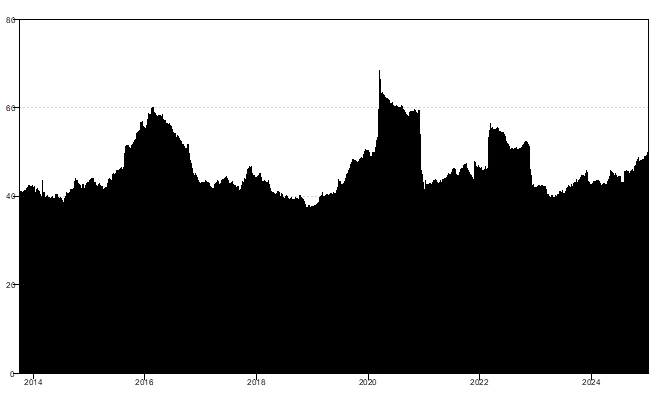
\includegraphics[width = 0.75\linewidth]{2aDynRetTCI}
      \end{subfigure}
\end{figure}
\begin{figure}[!htb]
\ContinuedFloat
      \begin{subfigure}[b]{\textwidth}
        \caption{Dynamic volatility TCI}
        \centering
        \label{fig:dynvolTCI}
        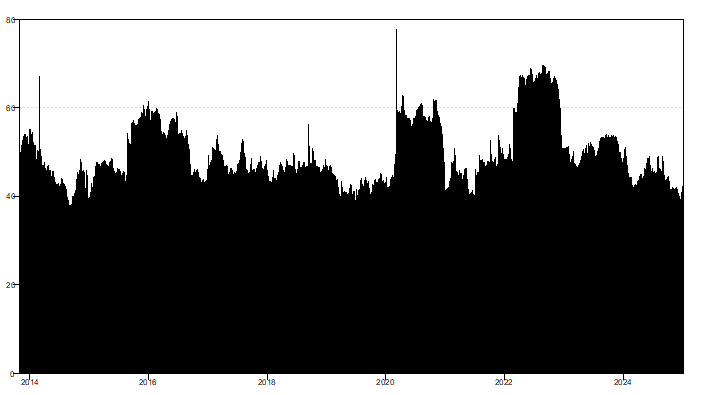
\includegraphics[width = 0.75\linewidth]{2bDynVolTCI}
      \end{subfigure}
\end{figure}

In contrast, the start of Phase IV in 2021 appears in the first instance
to have a lesser impact than these exogenous shocks with return
connectedness increasing at a much slower pace, though the effect seems
to be longer lasting as there has not been a persistent reversal to
date, if one disregards the Russia-Ukraine shock. The picture is a bit
more complicated with respect to volatility connectedness, whereby the
magnitude of the initial increase is again lower than the two shocks
that bookend the start of Phase IV, which is then followed by a steady
decline of this volatility connectedness below its long-run average.

Similarly, dynamic \textit{net} directional connectedness of EUAs with
other markets are provided in Figure \ref{fig:NDC} (\ref{apdx:NDC}
provides the complete set of charts). The charts indicate that during
Brexit vote the carbon's net connectedness of returns and volatility has
strengthened before reverting back closer to 0 by 2017. We observe a
similar pattern for the Covid-19 and Russia-Ukraine shocks. Curiously,
we also observe a similar pattern in 2018 for net return connectedness
and volatility. Although, there was not a definitive exogeneous shock,
these may be attributable to the broader signs of financial stress
around this period that witnessed escalating trade disputes, economic
downturn, particularly in China, and beginning of a pattern of rises in
interest rates with the Federal Reserve raising it four times in that
year.

\begin{figure}[!htb]
  \caption{Net Directional Connectedness between EUAs and other markets (Jan 2013 – Jan 2025)}
  \label{fig:NDC}
    \centering
      \begin{subfigure}[b]{\textwidth}
        \caption{Dynamic return net directional connectedness}
        \label{fig:dynretNDC}
        \centering
        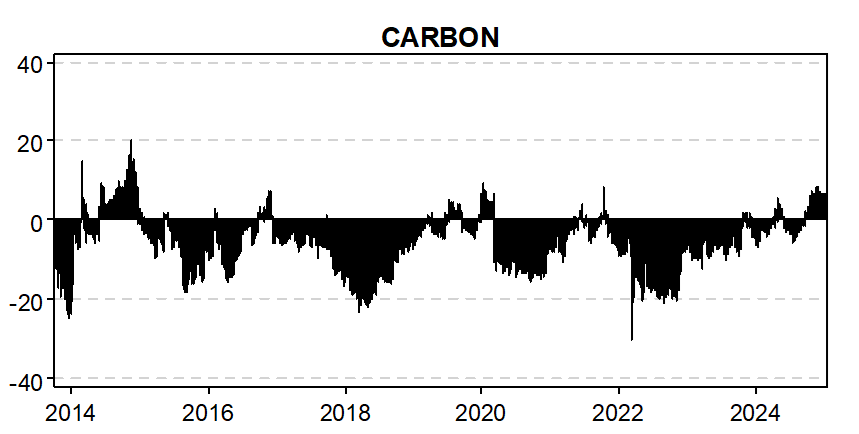
\includegraphics[width = 0.75\linewidth]{3aDynRetNDC}
      \end{subfigure}
\end{figure}
\begin{figure}[!htb]
\ContinuedFloat
      \begin{subfigure}[b]{\textwidth}
        \caption{Dynamic volatility net directional connectedness}
        \label{fig:dynvolNDC}
        \centering
        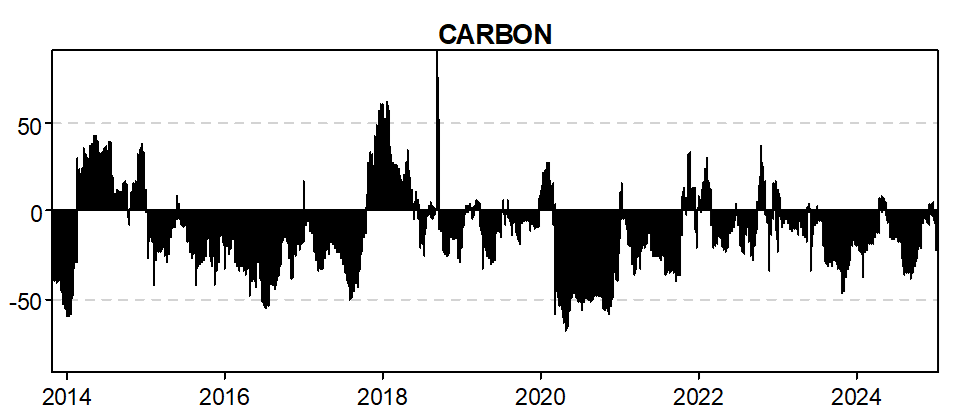
\includegraphics[width = 0.75\linewidth]{3bDynVolNDC}
      \end{subfigure}
\end{figure}

Overall, these net directional connectedness also suggest that in
periods of financial stress the return and volatility connectedness
between the EUAs and other markets increase. This seem to echo the
implications derived from the dynamic TCIs, though the latter looks only
at the total connectedness of the markets with each other, whereas here
we can ascertain the net connectedness of EUAs with other markets.
Importantly, in contrast to the EUAs' net return connectedness in panel
(a) that shows, for the mast part, EUAs as a receiver of return shocks
from other
markets,\footnote{Although, interestingly, we see a recent flip to net positive return connectedness towards the end of 2024}
panel (b) shows that the volatility net connectedness briefly flips to
positive in times of financial stress. Despite this increased
connectedness during financial stress, the change in the return
connectedness in these times is not only relatively small in magnitude
but also short lived. Thus it appears that EUAs can provide
diversification benefits to the portfolios both in good times and, when
shocks occur, albeit at a briefly reduced levels. Of course, not all
portfolios are alike. In order to better understand carbon market's
behavior with respect to individual markets we subsequently conduct
pairwise connectedness analysis.

\hypertarget{static-pairwise-connectedness}{%
\subsection{Static Pairwise
Connectedness}\label{static-pairwise-connectedness}}

TCI results are informative. However, as Section \ref{method}
highlighted, for networks with more than two variables, TCI tends to be
less efficient and accurate than PCI. PCI helps us break down the total
connectedness by measuring the level of connectedness between two
specific markets and quantifies how much the return or volatility
variation in one market is impacting, or being impacted by, the other
market.

Figure \ref{fig:statPCI} illustrates the network representation of PCI
where a line between markets means that a pairwise connectedness exists
between them with the thickness of the line indicating the magnitude of
such connectedness. For example, in panel (a) a strong pairwise
connectedness exists between European sovereign and corporate bond
returns, whereas such a pairwise connectedness between coal and natural
gas returns is weaker, and between either of the European bonds and coal
returns is inexistent. Panel (b) displays a similar interpretation for
volatility connectedness.

\begin{figure}[!htb]
  \caption{Network representation of Pairwise Connectedness Index (PCI) (Jan 2013 – Jan 2025)}
  \label{fig:statPCI}
    \centering
      \begin{subfigure}[a]{\textwidth}
        \caption{Static return PCI network}
        \label{fig:statretPCI}
        \centering
        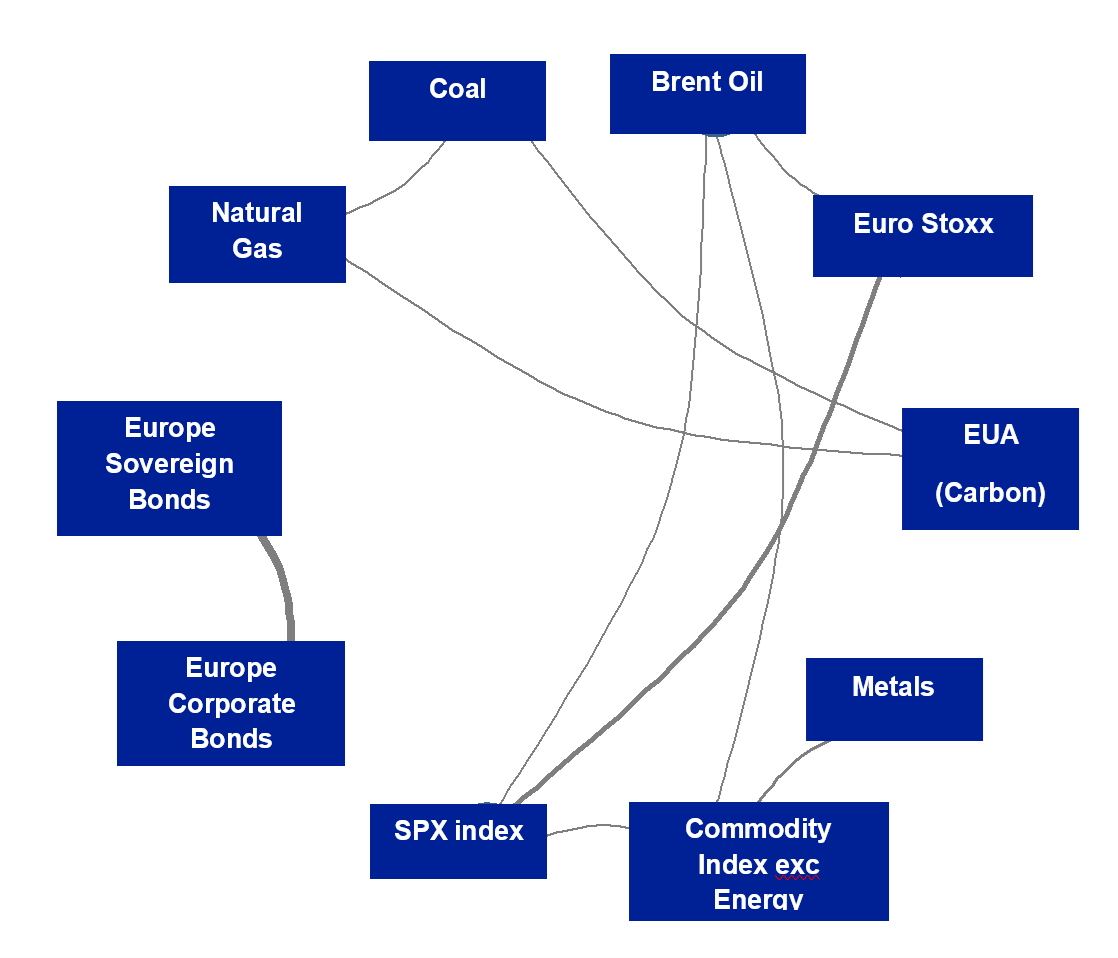
\includegraphics[width = 0.6\linewidth]{4aStatRetPCI}
      \end{subfigure}
\end{figure}
\begin{figure}[!htb]
\ContinuedFloat
      \begin{subfigure}[b]{\textwidth}
        \caption{Static volatility PCI network}
        \label{fig:statvolPCI}
        \centering
        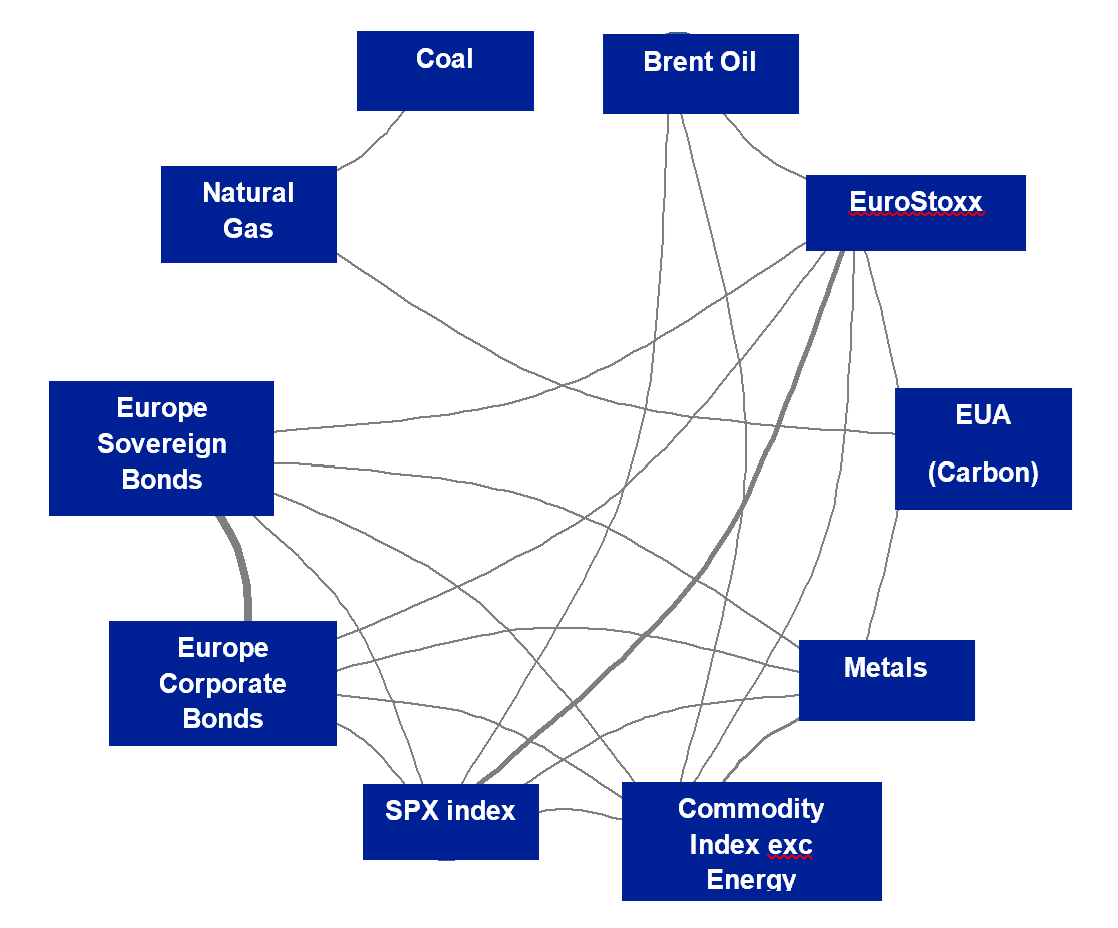
\includegraphics[width = 0.6\linewidth]{4bStatVolPCI}
      \end{subfigure}
\end{figure}

The PCI return connectedness network in panel (a) suggests that EUAs
seem to operate as an independent market, exhibiting pair connectedness
only with coal and natural gas, where there is also an equally weak
pairwise connection among coal and natural gas also. These could be
attributed to fuel switching in the power sector. Coal-to-gas switching
in the European energy market is a function of relative carbon and fuel
costs, driven by the EU ETS and fluctuating commodity prices. As EUA
prices rise the marginal cost of CO2 emissions increases, impacting coal
particularly due to its higher carbon intensity. This cost differential
incentivizes a shift towards gas-fired generation, which emits roughly
half the CO2 per unit of energy, creating a link between these markets.
However, the elasticity of this switch is contingent on natural gas
prices. When gas prices escalate the cost advantage of switching
diminishes, potentially leading utilities to revert to coal despite the
higher carbon costs, thereby increasing EUA demand and exerting upwards
pressure on EUA prices. Therefore, fluctuations in natural gas or coal
prices can alter the economic attractiveness of this fuel switch,
further reinforcing the connectedness. This would support the findings
of \citet{bertrand_carbon_2014}, \citet{hintermann_allowance_2010},
\citet{creti_carbon_2012}, and \citet{pettersson_fuel_2012} among
others.

The PCI volatility network in panel (b) reveals similar patterns, though
EUAs demonstrate volatility linkages with natural gas, as well as Stoxx
600 Index and Bloomberg Metal Commodity Index, but not with coal. This
observation of volatility connectedness not with coal but with natural
gas is supported by the findings of \citet{falbo_renewables_2019} and
\citet{bertrand_carbon_2014}, who argue that various EU initiatives and
policies aimed at increasing the share of renewables in the power grid
have led to EUAs being more closely linked with natural gas rather than
coal. This connection appears to persist despite a brief shift back to
coal during 2022, driven by the energy crisis caused by the
Russia-Ukraine war. This persistence in connections overlaps with
RePowerEU Plan which reinforces and accelerates the increase in share of
renewables. The volatility connectedness with Stoxx 600 and metals, on
the other hand, seems to support the observation of stronger total
connectedness in times of financial stress. In order to examine the
behavior of this over time, we next consider the dynamic pairwise
connectedness.

\hypertarget{dynamic-pairwise-connectedness}{%
\subsection{Dynamic Pairwise
Connectedness}\label{dynamic-pairwise-connectedness}}

When we examine the return and volatility PCI dynamically over time
(\ref{apdx:PCI} provides the full set of dynamic PCI charts), we see in
panel (a) of Figure \ref{fig:dynPCI} considerable fluctuations in EUAs'
pairwise return connectedness in times of crises.

\begin{figure}[!htb]
  \caption{Dynamic Return and Volatility Pairwise Connectedness Index (PCI) (Jan 2013 – Jan 2025)}
  \label{fig:dynPCI}
    \centering
      \begin{subfigure}[b]{\textwidth}
        \caption{Dynamic return PCI}
        \label{fig:dynretPCI}
        \centering
        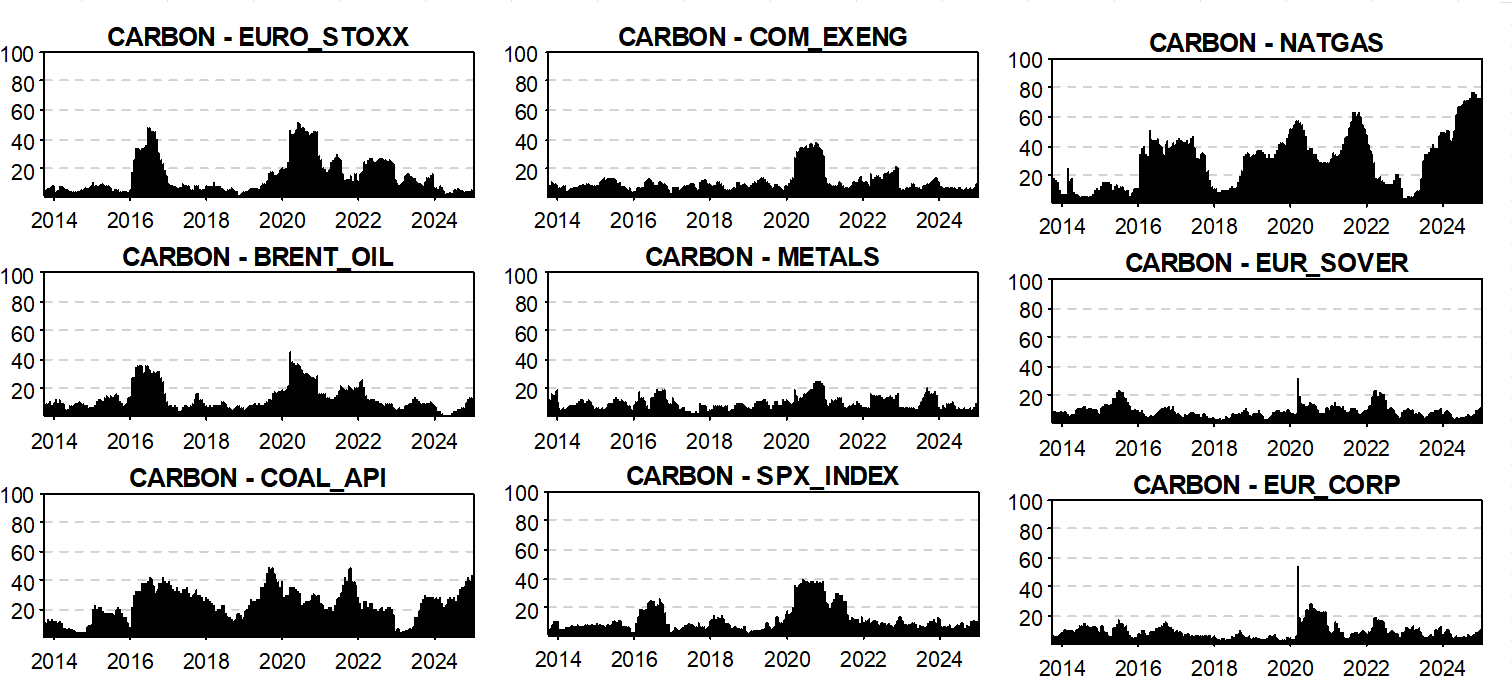
\includegraphics[width = 0.9\linewidth]{5aDynRetPCI}
      \end{subfigure}
\end{figure}
\begin{figure}[!htb]
\ContinuedFloat
      \begin{subfigure}[b]{\textwidth}
        \caption{Dynamic volatility PCI network}
        \label{fig:dynvolPCI}
        \centering
        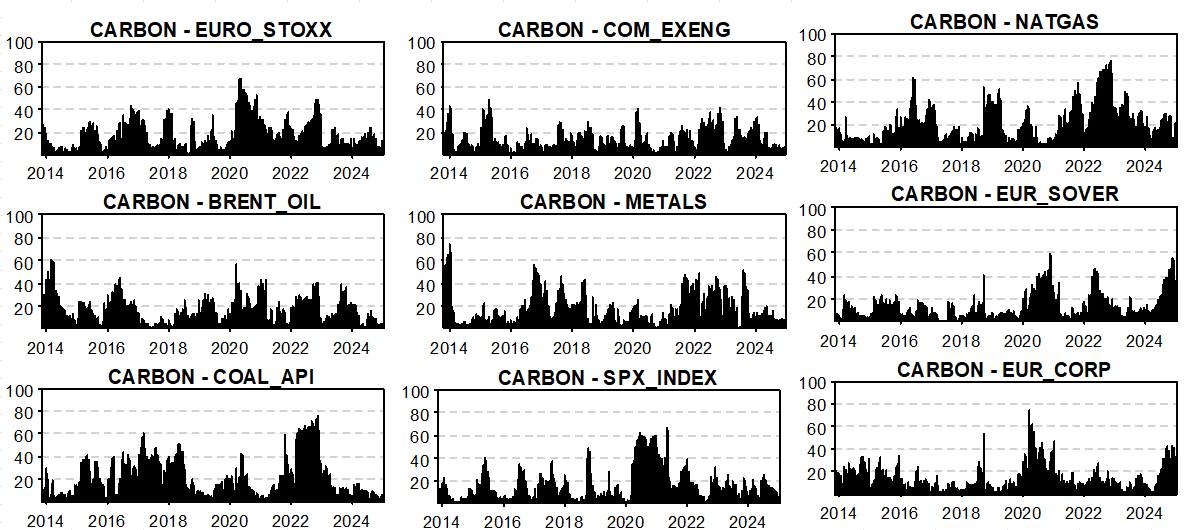
\includegraphics[width = 0.9\linewidth]{5bDynVolPCI}
      \end{subfigure}
\end{figure}

This appears to especially be the case with EuroStoxx, S\&P 500, brent,
coal, and natural gas which all spike to varying degrees around the
times of exogenous shocks such as the Brexit vote in 2016, Covid-19
crisis in 2020, and Russia-Ukraine war in 2022. A similar behavior is
observed, albeit to a lesser extent, with sovereign and corporate bonds,
metals and other commodities during these shocks. As it was observed in
the total connectedness most of these are short-lived. From these
dynamic PCI charts it also appears that coal and natural gas have
stronger return connectedness with the EUAs over time compared to other
markets.

There also seems to be a long-run incline in the return connectedness
between EUAs and natural gas, and a higher average connection with coal.
These changes may be attributable to various market, regulatory, and
policy factors. Especially from 2021 onwards, the introduction of Phase
IV and impacts of Fit for 55 and RePowerEU, which is accelerating the
deployment of renewable energy across Europe and helping the EU advance
its climate goals and reduce greenhouse gas emissions while also
diminishing reliance on Russian energy imports \citep{repowereu_2024},
may be contributing to this return connectedness behavior. Changes in
the energy mix, with a shift towards a relatively cleaner energy sources
including natural gas under the EU's climate targets and the Fit for 55
package can influence the demand for and price of EUAs, thus increasing
their connectedness. Coupling this with the impact of RepowerEU in the
acceleration of renewables capacity can strengthen such influence and
connectedness. Additionally, fluctuations in natural gas prices, due to
factors like supply disruptions or changes in demand, can directly
impact the cost-effectiveness of gas-fired power plants versus coal,
which would also affect the price and demand for EUAs. Furthermore, as
EU member states have been phasing out coal and adopting cleaner energy
sources, thereby reducing the influence of coal prices on the EUAs
market, there has been a regulatory push towards a reduced dependence on
coal, leading to gradual decrease in coal usage. These may explain why
EUA prices' link with coal are lower in strength than that of natural
gas.

Another important observation emerges on the return and volatility
connectedness between carbon and equity markets. While such
connectedness seems inexistent on the static return and volatility PCI
network in panels (a) and (b) of Figure \ref{fig:NDC}, we can observe in
the dynamic return and volatility PCI in Figure \ref{fig:dynPCI} that
such connectedness with Stoxx 600 Index and S\&P 500 Index seems to have
gained prominence around 2020. A similar pattern can also be observed
for EUAs connectedness with commodities and metals along with a brief
spike in bonds. Yet, it appears that among all pairwise connectedness
that gained prominence around 2020, only the return connectedness with
coal and natural gas is not short-lived, suggesting that broad
exogeneous shocks such as Covid-19 can briefly strengthen the
comnnectedness of carbon with other asset-classes.

The trend of strengthened connectedness with the equity markets may also
be due to the relatively recent introduction of financial products like
Exchange Traded Funds (ETFs) and other investment vehicles focusing on
carbon markets, including EUAs. These new products have broadened the
participation of financial investors who may be more responsive to
global macroeconomic shifts than specific carbon fundamentals. This
could lead to a strengthening of the return and volatility linkage
between EUAs and equities which would be a significant finding for
institutional investors looking to integrate EUAs into their portfolios.
However, the biggest seven ETFs have about EUR 430m assets under
management (AUM) in
total,\footnote{As of 31 January 2025, the largest seven ETFs on EUAs have a total AUM of EUR 428,695,211 with 5,154,000 total EUA holdings. These are, in descending order, SparkChange Physical Carbon EUA with AUM of EUR 148,604,300 and EUA holdings of 1,817,000; KRBN with AUM of EUR 129,364,862 and EUA holdings of 1,533,000; WisdomTree with AUM of EUR 83,862,474 and EUA holdings of 999,000; XEAL with AUM of EUR 29,878,322 and EUA holdings of 365,000; GRN with AUM of EUR 24,577,978 and EUA holdings of 293,000; KEUA with AUM of EUR 9,597,703 and EUA holdings of 114,000; and Horizons with AUM of EUR 2,809,572 and EUA holdings of 33,000.}
so the magnitude of the impact of this would inevitably be small.
Nevertheless the results of this study reveal that the overall
interconnectedness of EUAs with markets other than coal and natural gas
remains relatively low, reinforcing the potential diversification
benefits of including EUAs in investment portfolios, especially for
portfolios that exclude coal and natural gas. Such diversification
benefits, in turn, ought to incentivize financial institutions to
increase participation in the EU ETS and help further the EU's efforts
in decarbonization and transitioning into renewables.

\hypertarget{robustness-testing-of-connectedness-var-model-parameters}{%
\subsection{Robustness Testing of Connectedness (VAR) Model
Parameters}\label{robustness-testing-of-connectedness-var-model-parameters}}

We additionally test the robustness of the connectedness model
parameters following the methodology proposed by
\citet{wang_spillover_2023} by analyzing the sensitivity of the vector
autoregression (VAR) model's outcomes to changes in rolling window size
and forecast horizon. While the primary estimation utilized a rolling
window of 200 observations and a forecast horizon of 10 periods,
alternative configurations, including rolling window sizes of 180 and
220 observations and forecast horizons of 8 and 12 periods, were tested.
The results, detailed in \ref{apdx:Robust}, provide compelling evidence
supporting the reliability of the model.

The findings indicate that the total spillover index remains largely
stable across the alternative specifications, affirming the robustness
of the estimated spillover dynamics. Similarly, the pairwise
connectedness index (PCI) network structure exhibits minimal variation,
particularly emphasizing the return linkages between EUA carbon markets
with gas and coal markets. For volatility spillovers, a notable trend is
observed: as the forecast horizon of the VAR model is shortened, the
spillovers from EUA carbon markets to other markets decline, indicating
reduced volatility interdependence over shorter time frames.

These results are consistent across all tested rolling window sizes and
forecast horizons, confirming that the observed outcomes are not
sensitive to parameter variations. Consequently, the analysis validates
the study's conclusions regarding spillover effects among EUA carbon
markets and related markets. The stability of the metrics and network
structures further underscores the robustness and effectiveness of the
connectedness analysis in capturing intermarket relationships.

\hypertarget{conclusions}{%
\section{\texorpdfstring{Conclusions
\label{conclusion}}{Conclusions }}\label{conclusions}}

The EU has set an ambitious climate goal for 2030, committing to achieve
a 55\% reduction in GHG emissions relative to 1990 levels. In order to
meet this objective, the EU has adopted the Fit for 55 package, along
with the RepowerEU Plan. This aligns with a broader objective to
transform the EU into a sustainable economy and establish Europe as a
climate-neutral continent by 2050. A pivotal instrument in EU climate
policy is the EU-ETS, a cornerstone mechanism grounded on a
cap-and-trade system that limits and annually reduces emissions covered
by the system. The Fit for 55 package introduces reforms to the EU-ETS,
targeting a more aggressive reduction in the emission cap for the
high-emitting sectors covered by the system.

Various objectives underscore the necessity to tighten the cap, thereby
decreasing the supply of European Emission Allowances (EUAs). To that
end, this study sought to examine the financial characteristics of EUAs
to gain a more comprehensive understanding of this market and explore
whether EUAs can asssist the EU's climate goal by being a market for
diversification. Our findings show that in times of financial stress
returns and volatility of EUAs are briefly connected with equity markets
such as Stoxx 600 and S\&P 500, with European sovereign and corporate
bond markets, and with metals and non-energy commodity markets, but
become become less connected or altogether unconnected again relatively
quickly.

On the other hand, we see a stronger connection with the coal and
natural gas markets that is more pronounced during exogeneous shocks,
though again, short-lived. Nevertheless, it appears that there is a
stronger long-term connectedness with these markets - particularly from
2021 onwards - that are lower in magnitude compared to the impacts of
exogeneous shocks but longer in duration. These are likely due to
various market, regulatory, and policy factors that accelerate the
deployment of renewable energy and phasing out of coal. With the
introduction of Phase IV, Fit for 55 package, and RePowerEU Plan, there
is a drive to change the energy mix which would influence the demand
for, and price of, EUAs, which in turn would increase their
connectedness. A natural connection with these energy markets exists due
to significant participation of power generation in the EU-ETS. Yet the
relationship is complex due to fluctuations in natural gas prices that
at times makes fuel-switch to coal an attractive proposition, which, in
turn, would again impact the demand for, and price of, EUAs. Such
multilayered demand dynamics will inevitably engender a longer-lasting
linkages with energy markets. As a result, carbon markets would offer
diversification benefits that would likely to be more pronounced for
non-energy portfolios.

Overall, the results suggest that the return and volatility behavior of
EUAs are primarily driven by their own fundamental factors. For
investors, it suggests that EUAs could offer potential diversification
benefits when included in a portfolio, due to their low linkage and
spillover effect with other markets. These diversification benefits
would likely to be more acute for non-energy portfolios. By
incorporating EUAs, investors would not only increase their likelihood
of generating higher returns for a unit of volatility but also by
increasing the demand for EUAs, they would accelerate the
decarbonization efforts of the EU. We recommend, for future research,
investigating the behavior of non-energy and broad market portfolios
when carbon is incorporated at various densities in order to empirically
ascertain the magnitude of potential diversification benefits this asset
class offers.

\newpage

\appendix

\begin{landscape}
\section{Static Return and Volatility Connectedness Matrix} \label{apdx:ConnMatrix}
  \begin{table}[!ht]
    \caption{Static Return and Volatility Connectedness Matrix (Jan 2013 - Jan 2025)}
    \label{table:staticfull}
      \resizebox{\columnwidth}{!}{
      \begin{tabular}{|l|l|l|l|l|l|l|l|l|l|l|l|} 
        \multicolumn{12}{@{}l}{\em(a) Carbon returns connectedness matrix}\\ \hline
      & CARBON & EUROSTOXX & BRENT OIL & COAL API & NATGAS & EURSOVER & EURCORP & SPXINDEX & COMEXENG & METALS & DSF (FROM) \\ \hline
       CARBON & 60.06 & 4.00 & 3.80 &   7.85 & 10.21 & 2.48 &   2.26 & 3.47 &   2.76    & 3.11 & \textbf{39.94} \\ \hline
       EUROSTOXX & 3.28 &   49.76 & 5.70 & 3.33 &   3.12 & 3.05 &   3.67 & 19.87 & 5.20 &   3.03 & 50.24 \\ \hline
       BRENTOIL & 3.49 &    6.00 &  57.40 & 5.44 &  3.61 &  2.68 &  2.34 &  7.27 &  8.29 &  3.49 &  42.60 \\ \hline
       COALAPI & 6.34 & 3.77 &  5.80 &  56.02 & 13.78 & 1.85 &  2.04 &  3.84 &  3.96 &  2.62 &  43.98 \\ \hline
       NATGAS & 9.93 &  3.03 &  3.88 &  13.58 & 58.73 & 1.80 &  1.76 &  2.48 &  2.56 &  2.24 &  41.27 \\ \hline
       EURSOVER & 2.03 &    2.98 &  2.68 &  1.67 &  1.68 &  48.35 & 31.93 & 2.28 &  2.05 &  4.36 &  51.65 \\ \hline
       EURCORP & 1.97 & 5.05 &  2.71 &  1.75 & 1.81 &   30.37 & 45.49 & 3.97 &  2.54 &  4.35 &  54.51 \\ \hline
       SPXINDEX & 2.42 &    17.95 & 6.82 &  3.35 &  2.03 &  2.30 &  2.73 &  53.51 & 6.40 &  2.50 &  46.49 \\ \hline
       COMEXENG & 2.48 &    5.08 &  7.44 &  3.49 &  2.40 &  2.16 &  2.37 &  6.59 &  53.07 & 14.91 & 46.93 \\ \hline
       METALS & 2.37 &  3.15 &  3.10 &  2.28 &  2.47 &  4.83 &  5.59 &  2.96 &  16.14 & 57.11 & 42.89 \\ \hline
       DST (TO) & \textbf{34.31} & 51.01 &  41.93 & 42.73 & 41.10 & 51.52 & 54.69 & 52.73 & 49.89 & 40.60 & 460.50 \\ \hline
       Inc.Own & 94.37 & 100.77 &   99.33 & 98.75 & 99.83 & 99.87 & 100.18 &    106.24 &    102.96 &    97.70 & \textbf{TCI} \\ \hline
       NS (NET) & \textbf{-5.63} & 0.77 &   -0.67 & -1.25 & -0.17 & -0.13 & 0.18 &  6.24 &  2.96 &  -2.30 & \textbf{46.05} \\ \hline
        \end{tabular}
        }
\bigskip\bigskip
         \resizebox{\columnwidth}{!}{
         \begin{tabular}{|l|l|l|l|l|l|l|l|l|l|l|l|} 
          \multicolumn{12}{@{}l}{\em(b) Carbon volatility connectedness matrix}\\ \hline
       & CARBON & EUROSTOXX & BRENTOIL & COALAPI & NATGAS & EURSOVER & EURCORP & SPXINDEX & COMEXENG & METALS & DSF (FROM) \\ \hline
       CARBON & 55.66 & 4.60 &  4.29 &  7.25 &  7.13 &  3.77 &  3.61 &  5.06 &  3.83 &  4.79 & \textbf{44.34} \\ \hline
       EUROSTOXX & 3.63 &   47.09 & 5.17 & 3.59 &   3.45 &  5.12 &  4.14 &  16.60 & 5.25 &  5.95 &  52.91 \\ \hline
       BRENTOIL & 4.20 &    6.54 &  52.55 & 4.93 &  3.59 &  3.85 &  4.54 &  6.49 &  7.10 &  6.20 &  47.45 \\ \hline
       COALAPI & 4.67 & 5.83 &  4.19 &  57.95 & 7.85 &  3.80 &  2.71 &  4.59 &  3.14 &  5.26 &  42.05 \\ \hline
       NATGAS & 4.51 &  4.64 &  3.43 &  8.36 &  59.40 & 3.52 &  3.79 &  4.82 &  3.56 &  3.96 &  40.60 \\ \hline
       EURSOVER & 2.17 &    6.27 &  3.30 &  2.43 &  1.86 &  44.69 & 25.39 & 5.60 & 3.86 &   4.44 &  55.31 \\ \hline
       EURCORP & 2.81 & 5.70 &  2.52 &  2.34 &  2.40 &  28.32 & 41.90 & 5.97 &  4.70 &  3.33 &  58.10 \\ \hline
       SPXINDEX & 3.29 &    15.44 & 5.03 &  3.08 &  1.71 &  4.71 &  3.98 &  53.15 & 4.44 &  5.17 &  46.85 \\ \hline
       COMEXENG & 2.62 &    7.96 &  4.69 &  3.94 &  4.00 &  5.32 &  5.39 &  6.71 &  49.30 & 10.07 & 50.70 \\ \hline
       METALS & 3.91 &  8.31 &  4.44 &  3.90 &  3.85 &  5.08 &  6.31 &  6.26 &  10.05 & 47.90 & 52.10 \\ \hline
       DST (TO) & \textbf{31.83} & 65.30 &  37.07 & 39.82 & 35.85 & 63.47 & 59.86 & 62.11 & 45.92 & 49.18 & 490.40 \\ \hline
       Inc.Own & 87.49 &    112.39 &    89.62 & 97.77 & 95.25 & 108.16 &    101.76 &    115.27 &    95.22   & 97.08 & \textbf{TCI} \\ \hline
       NS (NET) & \textbf{-12.51} & 12.39 & -10.38 &    -2.23 & -4.75 & 8.16 &  1.76 &  15.27 & -4.78 & -2.92 & \textbf{49.04} \\ \hline
        \end{tabular}
        }
\end{table}




\section{Dynamic Return and Volatility Net Directional Connectedness}  \label{apdx:NDC}
\begin{figure}[H]
  \caption{Dynamic Net Directional Connectedness (Jan 2013 – Jan 2025)}
  \label{fig:dynNDCfull}
    \centering
      \begin{subfigure}[a]{\textwidth}
        \caption{Dynamic return net directional connectedness}
        \label{fig:dynretNDCfull}
        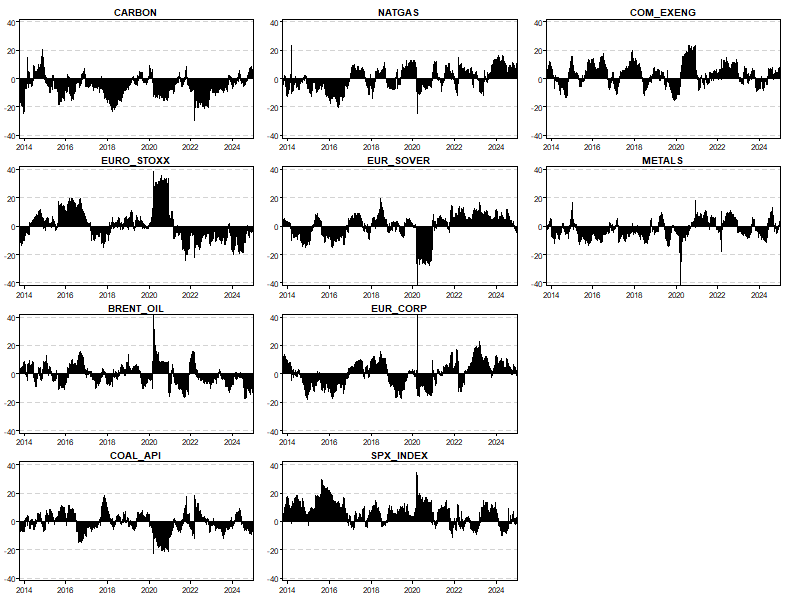
\includegraphics[width = 1.25\linewidth]{6aApdxB-DynRetNDCfull}
      \end{subfigure}
\end{figure}
\begin{figure}[H]
  \ContinuedFloat
  \centering
      \begin{subfigure}[b]{\textwidth}
        \caption{Dynamic volatility net directional connectedness}
        \label{fig:dynvolNDCfull}
        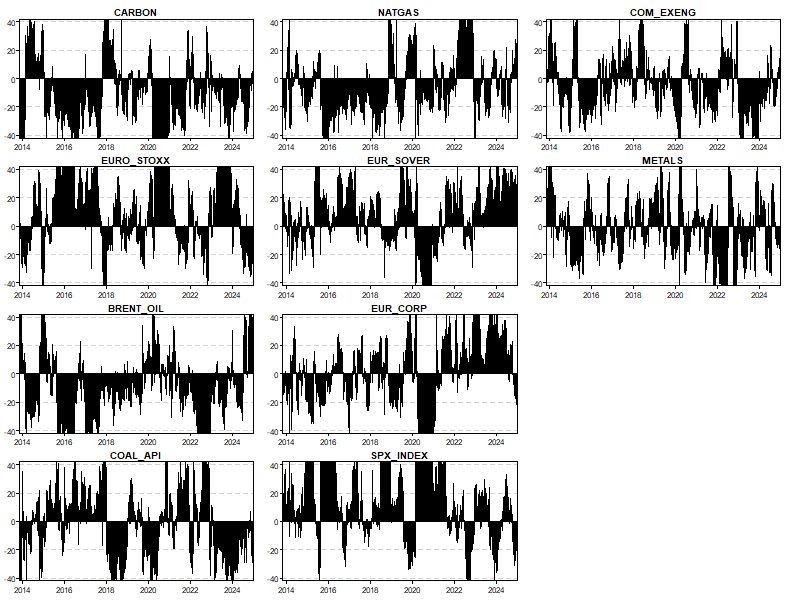
\includegraphics[width = 1.25\linewidth]{6bApdxB-DynVolNDCfull}
      \end{subfigure}
\end{figure}

\newpage

\section{Dynamic Return and Volatility Pairwise Connectedness Index} \label{apdx:PCI}
\begin{figure}[!ht]
  \caption{Dynamic Return and Volatility Pairwise Connectedness Index (Jan 2013 – Jan 2025)}
  \label{fig:dynPCIfull}
  \centering
  \begin{subfigure}[a]{\textwidth}
    \caption{Dynamic return PCI}
    \label{fig:dynretPCIfull}
    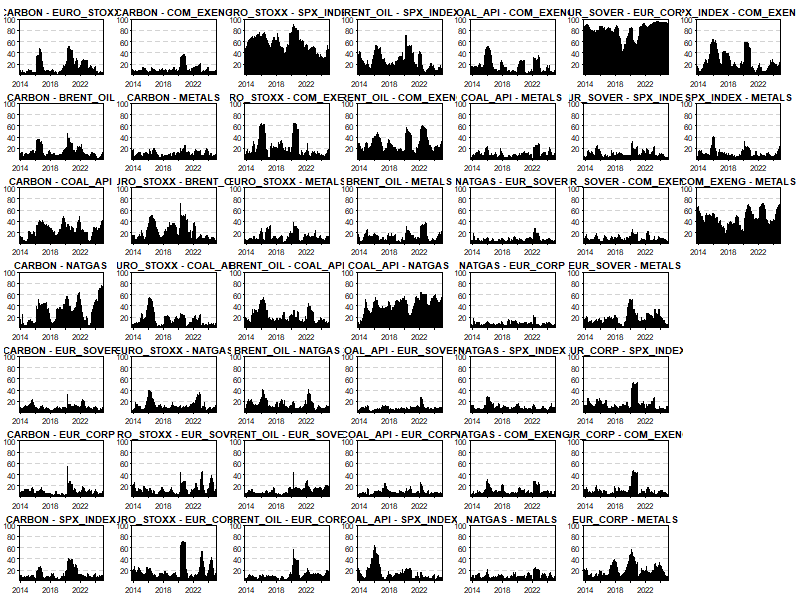
\includegraphics[width = 1.1\linewidth]{7aApdxC-DynRetPCIfull}
  \end{subfigure}
\end{figure}
\begin{figure}[!ht]
  \ContinuedFloat
  \centering
    \begin{subfigure}[b]{\textwidth}\ContinuedFloat
      \caption{Dynamic volatility PCI}
      \label{fig:dynvolPCIfull}
      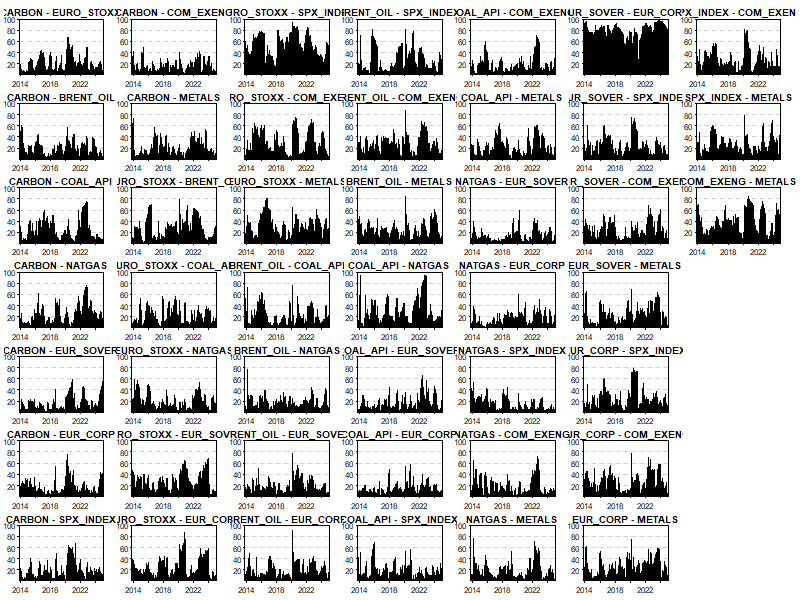
\includegraphics[width = 1.2\linewidth]{7bApdxC-DynVolPCIfull}
    \end{subfigure}
\end{figure}


\newpage

\section{Robustness Testing of Connectedness Model Parameters} \label{apdx:Robust}
\subsection{10-period forecast horizon and a rolling window of 180 observations}

\subsubsection{Static Return and Volatility Connectedness Matrix}

  \begin{table}[!ht]
    \caption{Static Return and Volatility Connectedness Matrix (Jan 2013 - Jan 2025)}
      \resizebox{\columnwidth}{!}{
      \begin{tabular}{|l|l|l|l|l|l|l|l|l|l|l|l|}
      \multicolumn{12}{@{}l}{\em(a) Carbon returns connectedness matrix}\\ \hline
        ~ & CARBON & EUROSTOXX & BRENTOIL & COALAPI & NATGAS & EURSOVER & EURCORP & SPXINDEX & COMEXENG & METALS & FROM \\ \hline
        CARBON & 58.42 & 4.13 & 3.95 & 7.9 & 10.32 & 2.75 & 2.49 & 3.71 & 2.96 & 3.37 & 41.58 \\ \hline
        EUROSTOXX & 3.42 & 48.5 & 5.77 & 3.45 & 3.35 & 3.4 & 3.94 & 19.55 & 5.3 & 3.32 & 51.5 \\ \hline
        BRENTOIL & 3.73 & 6.14 & 56.08 & 5.53 & 3.75 & 2.88 & 2.51 & 7.34 & 8.26 & 3.78 & 43.92 \\ \hline
        COALAPI & 6.47 & 3.92 & 5.88 & 54.74 & 13.63 & 2.07 & 2.25 & 4.02 & 4.11 & 2.91 & 45.26 \\ \hline
        NATGAS & 10.05 & 3.24 & 4.05 & 13.36 & 57.16 & 2.07 & 1.99 & 2.76 & 2.82 & 2.49 & 42.84 \\ \hline
        EURSOVER & 2.25 & 3.24 & 2.94 & 1.89 & 1.94 & 47.16 & 31.34 & 2.45 & 2.3 & 4.48 & 52.84 \\ \hline
        EURCORP & 2.18 & 5.15 & 2.89 & 1.98 & 2.05 & 29.92 & 44.6 & 4.04 & 2.7 & 4.48 & 55.4 \\ \hline
        SPXINDEX & 2.62 & 17.77 & 6.93 & 3.49 & 2.29 & 2.53 & 2.92 & 52.31 & 6.39 & 2.75 & 47.69 \\ \hline
        COMEXENG & 2.68 & 5.17 & 7.47 & 3.64 & 2.68 & 2.41 & 2.56 & 6.59 & 51.98 & 14.82 & 48.02 \\ \hline
        METALS & 2.58 & 3.42 & 3.38 & 2.51 & 2.73 & 4.92 & 5.67 & 3.2 & 15.94 & 55.65 & 44.35 \\ \hline
        DST(TO) & 35.98 & 52.19 & 43.28 & 43.75 & 42.74 & 52.95 & 55.68 & 53.66 & 50.79 & 42.39 & 473.4 \\ \hline
        Inc. Own & 94.41 & 100.69 & 99.36 & 98.49 & 99.9 & 100.11 & 100.28 & 105.96 & 102.76 & 98.04 & cTCI/TCI \\ \hline
        NS (NET) & -5.59 & 0.69 & -0.64 & -1.51 & -0.1 & 0.11 & 0.28 & 5.96 & 2.76 & -1.96 & 52.60/47.34 \\ \hline
    \end{tabular}
    }
    \bigskip
      \resizebox{\columnwidth}{!}{
      \begin{tabular}{|l|l|l|l|l|l|l|l|l|l|l|l|}
      \multicolumn{12}{@{}l}{\em(b) Carbon volatility connectedness matrix}\\ \hline
        ~ & CARBON & EUROSTOXX & BRENTOIL & COALAPI & NATGAS & EURSOVER & EURCORP & SPXINDEX & COMEXENG & METALS & FROM \\ \hline
        CARBON & 52.95 & 4.7 & 4.74 & 7.16 & 7.63 & 4.19 & 3.79 & 5.42 & 4.13 & 5.3 & 47.05 \\ \hline
        EUROSTOXX & 4.01 & 45.08 & 5.34 & 4.25 & 3.87 & 5.52 & 4.38 & 15.91 & 5.33 & 6.3 & 54.92 \\ \hline
        BRENTOIL & 4.76 & 6.68 & 49.8 & 5.09 & 3.85 & 4.3 & 4.99 & 6.78 & 7.12 & 6.64 & 50.2 \\ \hline
        COALAPI & 4.88 & 6.1 & 4.69 & 54.65 & 8.24 & 4.24 & 3.12 & 5.11 & 3.45 & 5.52 & 45.35 \\ \hline
        NATGAS & 4.74 & 4.99 & 3.73 & 8.42 & 56.56 & 3.94 & 3.96 & 5.28 & 4.05 & 4.33 & 43.44 \\ \hline
        EURSOVER & 2.49 & 6.48 & 3.6 & 2.86 & 2.38 & 42.69 & 24.76 & 5.84 & 4.43 & 4.47 & 57.31 \\ \hline
        EURCORP & 3.24 & 5.76 & 2.65 & 2.84 & 3 & 27.52 & 39.98 & 6.12 & 5.26 & 3.63 & 60.02 \\ \hline
        SPXINDEX & 3.54 & 15.08 & 5.4 & 3.42 & 2.05 & 5.22 & 4.41 & 50.56 & 4.69 & 5.63 & 49.44 \\ \hline
        COMEXENG & 3.18 & 7.91 & 4.75 & 4.33 & 4.51 & 6.08 & 5.78 & 7.11 & 46.34 & 10 & 53.66 \\ \hline
        METALS & 4.27 & 8.4 & 4.76 & 4.29 & 4.33 & 5.28 & 6.78 & 6.91 & 9.64 & 45.33 & 54.67 \\ \hline
        DST(TO) & 35.11 & 66.11 & 39.64 & 42.67 & 39.87 & 66.29 & 61.97 & 64.48 & 48.1 & 51.81 & 516.05 \\ \hline
        Inc. Own & 88.06 & 111.19 & 89.44 & 97.33 & 96.43 & 108.98 & 101.96 & 115.04 & 94.45 & 97.14 & cTCI/TCI \\ \hline
        NS (NET) & -11.94 & 11.19 & -10.56 & -2.67 & -3.57 & 8.98 & 1.96 & 15.04 & -5.55 & -2.86 & 57.34/51.60 \\ \hline
    \end{tabular}
    }
\end{table}




\subsubsection{Dynamic Return and Volatility Net Directional Connectedness}

\begin{figure}[H]
  \caption{Dynamic Net Directional Connectedness (Jan 2013 – Jan 2025)}
    \centering
      \begin{subfigure}[a]{\textwidth}
        \caption{Dynamic return net directional connectedness}
        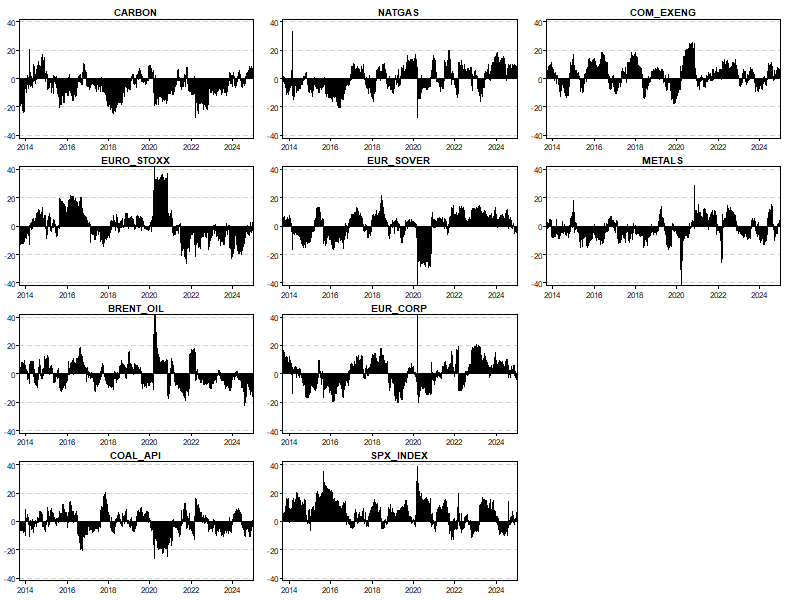
\includegraphics[width = 1.25\linewidth]{8aApdxD-10-180-RetNDC}
      \end{subfigure}
\end{figure}
\begin{figure}[H]
  \ContinuedFloat
  \centering
      \begin{subfigure}[b]{\textwidth}
        \caption{Dynamic volatility net directional connectedness}
        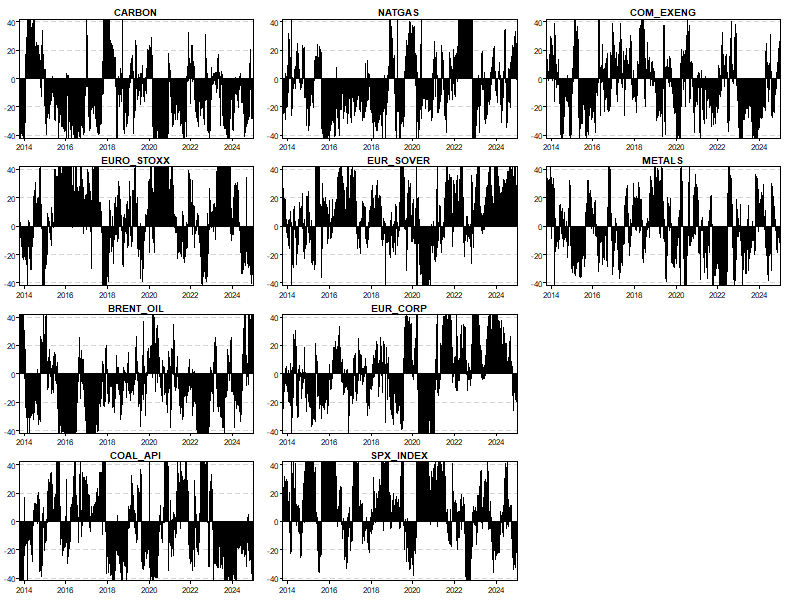
\includegraphics[width = 1.25\linewidth]{8bApdxD-10-180-VolNDC}
      \end{subfigure}
\end{figure}



\subsubsection{Static Return and Volatility Pairwise Directional Connectedness}

\begin{figure}[!ht]
  \caption{Network Representation of Pairwise Connectedness Index (Jan 2013 – Jan 2025)}
  \begin{minipage}{.8\textwidth}
    \subfloat[Static Return PCI network]{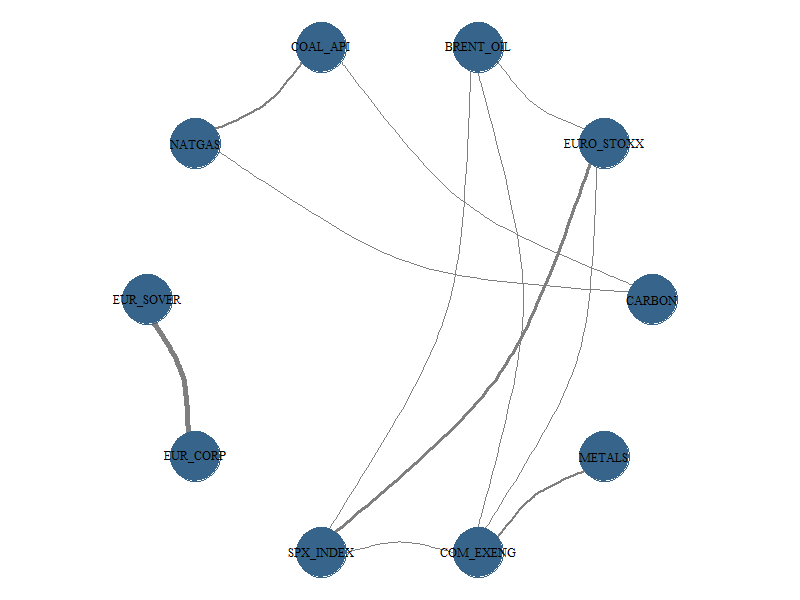
\includegraphics[width = \linewidth]{9aApdxD-10-180-RetNtwrk}}
  \end{minipage}
  \hfill
  \begin{minipage}{.8\textwidth}
    \subfloat[Static Volatility PCI network]{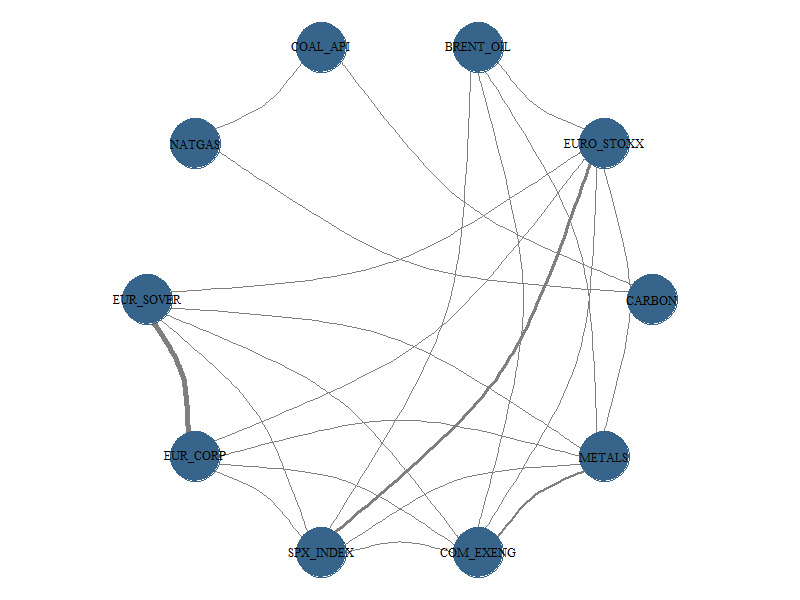
\includegraphics[width = \linewidth]{9bApdxD-10-180-VolNtwrk}}
  \end{minipage}
\end{figure}



\newpage

\subsubsection{Dynamic Return and Volatility Pairwise Directional Connectedness}

\begin{figure}[!ht]
  \caption{Dynamic Return and Volatility Pairwise Connectedness Index (Jan 2013 – Jan 2025)}
  \centering
  \begin{subfigure}[a]{\textwidth}
    \caption{Dynamic return PCI}
    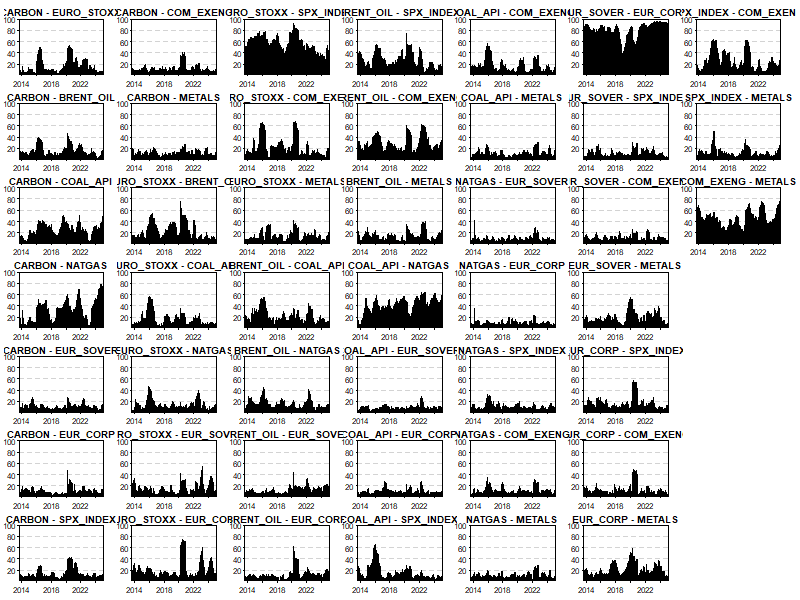
\includegraphics[width = 1.1\linewidth]{10aApdxD-10-180-RetPCI}
  \end{subfigure}
\end{figure}
\begin{figure}[!ht]
  \ContinuedFloat
  \centering
    \begin{subfigure}[b]{\textwidth}\ContinuedFloat
      \caption{Dynamic volatility PCI}
      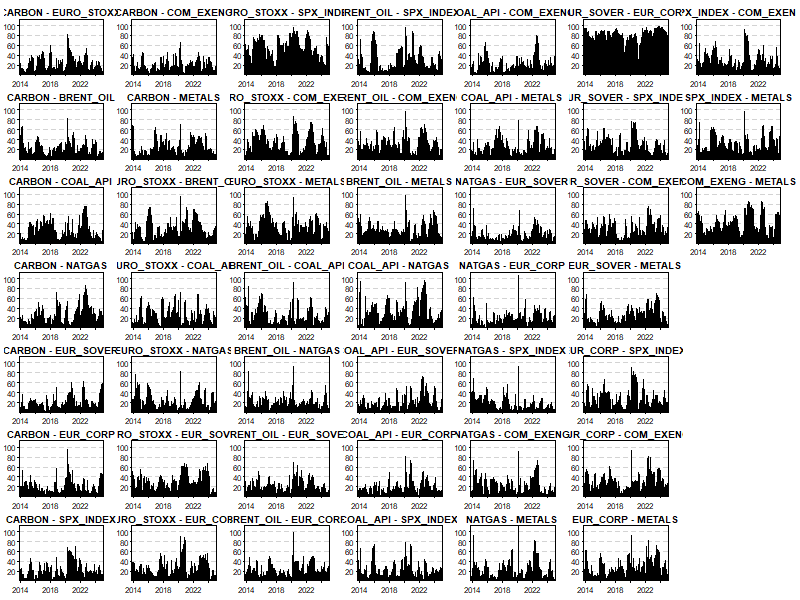
\includegraphics[width = 1.2\linewidth]{10bApdxD-10-180-VolPCI}
    \end{subfigure}
\end{figure}





\subsection{10-period forecast horizon and a rolling window of 220 observations}

\subsubsection{Static Return and Volatility Connectedness Matrix}

  \begin{table}[!ht]
    \caption{Static Return and Volatility Connectedness Matrix (Jan 2013 - Jan 2025)}
      \resizebox{\columnwidth}{!}{
      \begin{tabular}{|l|l|l|l|l|l|l|l|l|l|l|l|}
    \multicolumn{12}{@{}l}{\em(a) Carbon returns connectedness matrix}\\ \hline
        ~ & CARBON & EUROSTOXX & BRENTOIL & COALAPI & NATGAS & EURSOVER & EURCORP & SPXINDEX & COMEXENG & METALS & FROM \\ \hline
        CARBON & 61.35 & 3.93 & 3.67 & 7.77 & 10.07 & 2.29 & 2.12 & 3.28 & 2.6 & 2.91 & 38.65 \\ \hline
        EUROSTOXX & 3.17 & 50.79 & 5.67 & 3.23 & 2.94 & 2.75 & 3.43 & 20.12 & 5.14 & 2.77 & 49.21 \\ \hline
        BRENTOIL & 3.31 & 5.91 & 58.43 & 5.38 & 3.49 & 2.5 & 2.22 & 7.19 & 8.32 & 3.25 & 41.57 \\ \hline
        COALAPI & 6.21 & 3.65 & 5.74 & 57.04 & 13.87 & 1.71 & 1.88 & 3.69 & 3.82 & 2.38 & 42.96 \\ \hline
        NATGAS & 9.8 & 2.86 & 3.74 & 13.76 & 59.97 & 1.62 & 1.6 & 2.23 & 2.37 & 2.05 & 40.03 \\ \hline
        EURSOVER & 1.86 & 2.78 & 2.47 & 1.5 & 1.47 & 49.32 & 32.36 & 2.14 & 1.84 & 4.25 & 50.68 \\ \hline
        EURCORP & 1.83 & 5 & 2.6 & 1.56 & 1.6 & 30.68 & 46.15 & 3.92 & 2.43 & 4.22 & 53.85 \\ \hline
        SPXINDEX & 2.25 & 18.12 & 6.71 & 3.21 & 1.8 & 2.12 & 2.58 & 54.48 & 6.44 & 2.29 & 45.52 \\ \hline
        COMEXENG & 2.32 & 5.03 & 7.42 & 3.34 & 2.17 & 1.96 & 2.21 & 6.63 & 53.93 & 14.98 & 46.07 \\ \hline
        METALS & 2.21 & 2.9 & 2.88 & 2.07 & 2.24 & 4.77 & 5.5 & 2.76 & 16.3 & 58.36 & 41.64 \\ \hline
        DST(TO) & 32.96 & 50.19 & 40.89 & 41.83 & 39.66 & 50.41 & 53.92 & 51.95 & 49.25 & 39.11 & 450.17 \\ \hline
        Inc. Own & 94.31 & 100.98 & 99.31 & 98.87 & 99.63 & 99.74 & 100.08 & 106.43 & 103.18 & 97.48 & cTCI/TCI \\ \hline
        NS (NET) & -5.69 & 0.98 & -0.69 & -1.13 & -0.37 & -0.26 & 0.08 & 6.43 & 3.18 & -2.52 & 50.02/45.02 \\ \hline
    \end{tabular}
    }
    \bigskip
      \resizebox{\columnwidth}{!}{
      \begin{tabular}{|l|l|l|l|l|l|l|l|l|l|l|l|}
    \multicolumn{12}{@{}l}{\em(b) Carbon volatility connectedness matrix}\\ \hline
        ~ & CARBON & EUROSTOXX & BRENTOIL & COALAPI & NATGAS & EURSOVER & EURCORP & SPXINDEX & COMEXENG & METALS & FROM \\ \hline
        CARBON & 57.82 & 4.6 & 3.99 & 7.25 & 6.77 & 3.43 & 3.28 & 4.71 & 3.77 & 4.37 & 42.18 \\ \hline
        EUROSTOXX & 3.26 & 48.44 & 4.96 & 3.2 & 3.12 & 4.95 & 4.06 & 17.08 & 5.26 & 5.68 & 51.56 \\ \hline
        BRENTOIL & 3.71 & 6.49 & 54.56 & 4.78 & 3.39 & 3.48 & 4.09 & 6.32 & 7.29 & 5.9 & 45.44 \\ \hline
        COALAPI & 4.61 & 5.41 & 3.49 & 60.67 & 7.47 & 3.55 & 2.54 & 4.17 & 3 & 5.09 & 39.33 \\ \hline
        NATGAS & 4.33 & 4.33 & 3.04 & 8.15 & 62.01 & 3.2 & 3.63 & 4.47 & 3.24 & 3.6 & 37.99 \\ \hline
        EURSOVER & 1.88 & 6.07 & 3.1 & 2.09 & 1.59 & 46.2 & 25.84 & 5.5 & 3.43 & 4.3 & 53.8 \\ \hline
        EURCORP & 2.48 & 5.69 & 2.46 & 1.93 & 1.95 & 28.91 & 43.34 & 5.93 & 4.14 & 3.17 & 56.66 \\ \hline
        SPXINDEX & 3.03 & 15.53 & 4.64 & 2.83 & 1.51 & 4.32 & 3.72 & 55.36 & 4.18 & 4.88 & 44.64 \\ \hline
        COMEXENG & 2.16 & 7.92 & 4.69 & 3.69 & 3.6 & 4.81 & 4.93 & 6.45 & 51.6 & 10.15 & 48.4 \\ \hline
        METALS & 3.68 & 8.12 & 4.08 & 3.63 & 3.45 & 4.91 & 5.83 & 5.71 & 10.35 & 50.22 & 49.78 \\ \hline
        DST(TO) & 29.15 & 64.17 & 34.46 & 37.57 & 32.84 & 61.55 & 57.91 & 60.35 & 44.66 & 47.14 & 469.8 \\ \hline
        Inc. Own & 86.97 & 112.61 & 89.02 & 98.23 & 94.85 & 107.74 & 101.25 & 115.71 & 96.26 & 97.36 & cTCI/TCI \\ \hline
        NS (NET) & -13.03 & 12.61 & -10.98 & -1.77 & -5.15 & 7.74 & 1.25 & 15.71 & -3.74 & -2.64 & 52.20/46.98 \\ \hline
    \end{tabular}
    }
\end{table}




\subsubsection{Dynamic Return and Volatility Net Directional Connectedness}

\begin{figure}[H]
  \caption{Dynamic Net Directional Connectedness (Jan 2013 – Jan 2025)}
    \centering
      \begin{subfigure}[a]{\textwidth}
        \caption{Dynamic return net directional connectedness}
        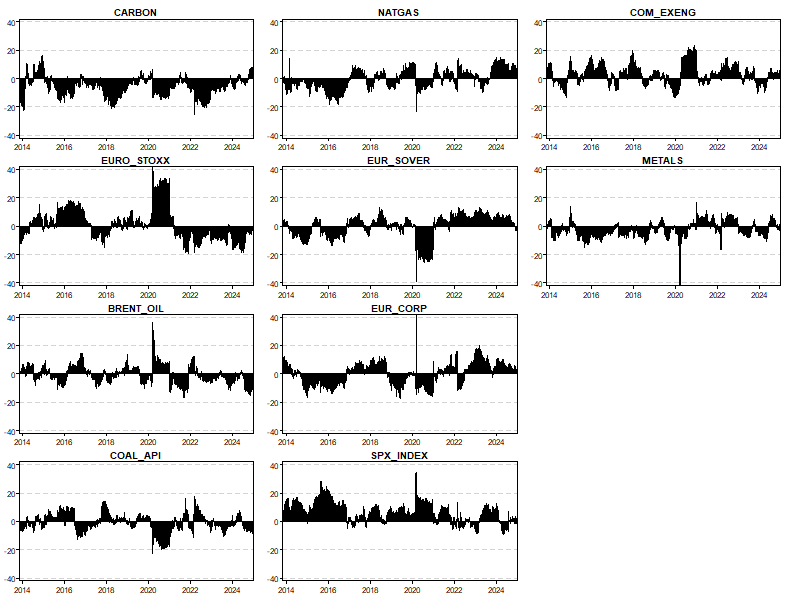
\includegraphics[width = 1.25\linewidth]{11aApdxD-10-220-RetNDC}
      \end{subfigure}
\end{figure}
\begin{figure}[H]
  \ContinuedFloat
  \centering
      \begin{subfigure}[b]{\textwidth}
        \caption{Dynamic volatility net directional connectedness}
        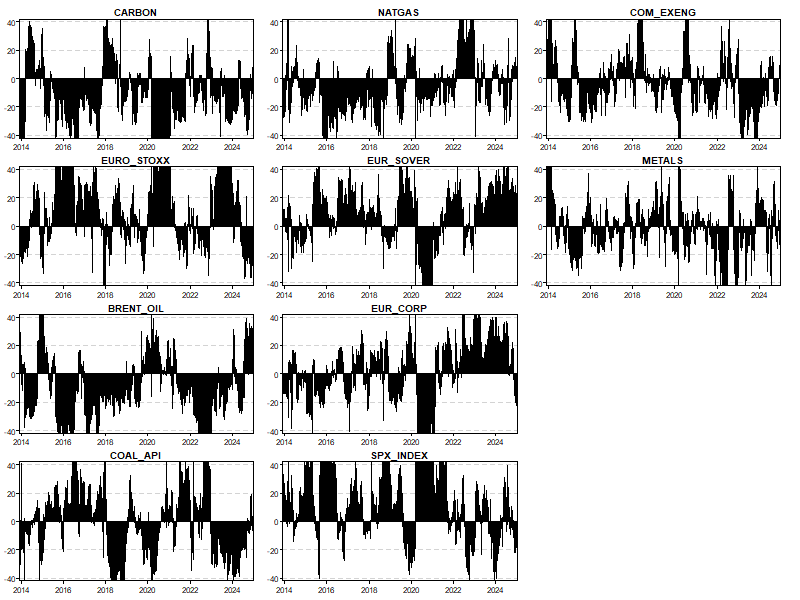
\includegraphics[width = 1.25\linewidth]{11bApdxD-10-220-VolNDC}
      \end{subfigure}
\end{figure}



\subsubsection{Static Return and Volatility Pairwise Directional Connectedness}

\begin{figure}[!ht]
  \caption{Network Representation of Pairwise Connectedness Index (Jan 2013 – Jan 2025)}
  \begin{minipage}{.8\textwidth}
    \subfloat[Static Return PCI network]{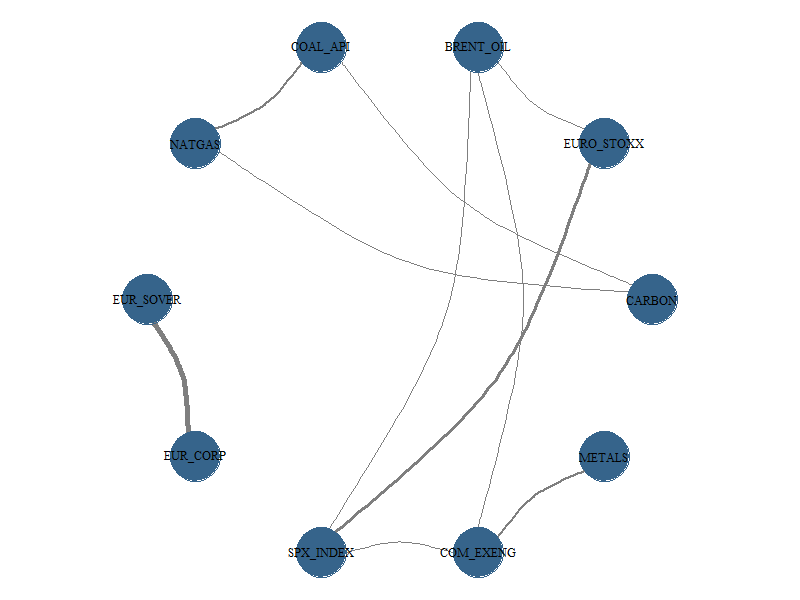
\includegraphics[width = \linewidth]{12aApdxD-10-220-RetNtwrk}}
  \end{minipage}
  \hfill
  \begin{minipage}{.8\textwidth}
    \subfloat[Static Volatility PCI network]{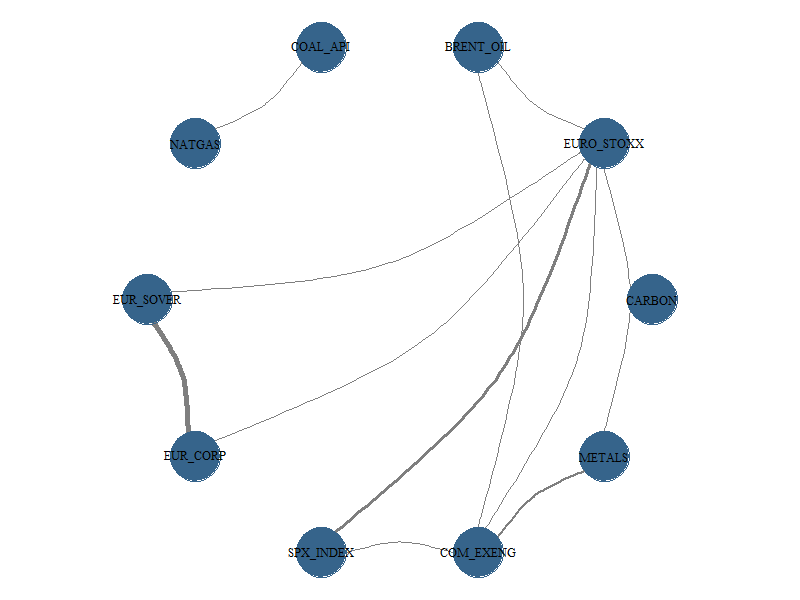
\includegraphics[width = \linewidth]{12bApdxD-10-220-VolNtwrk}}
  \end{minipage}
\end{figure}



\newpage

\subsubsection{Dynamic Return and Volatility Pairwise Directional Connectedness}

\begin{figure}[!ht]
  \caption{Dynamic Return and Volatility Pairwise Connectedness Index (Jan 2013 – Jan 2025)}
  \centering
  \begin{subfigure}[a]{\textwidth}
    \caption{Dynamic return PCI}
    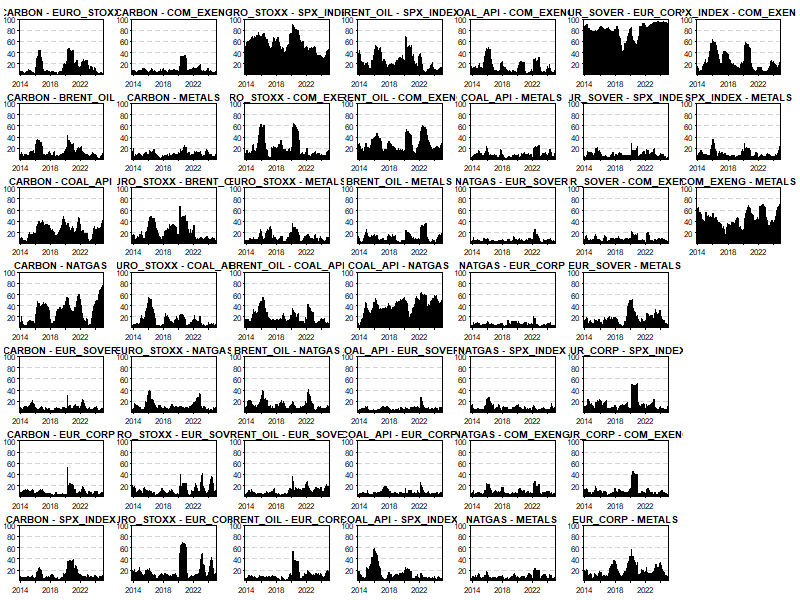
\includegraphics[width = 1.1\linewidth]{13aApdxD-10-220-RetPCI}
  \end{subfigure}
\end{figure}
\begin{figure}[!ht]
  \ContinuedFloat
  \centering
    \begin{subfigure}[b]{\textwidth}\ContinuedFloat
      \caption{Dynamic volatility PCI}
      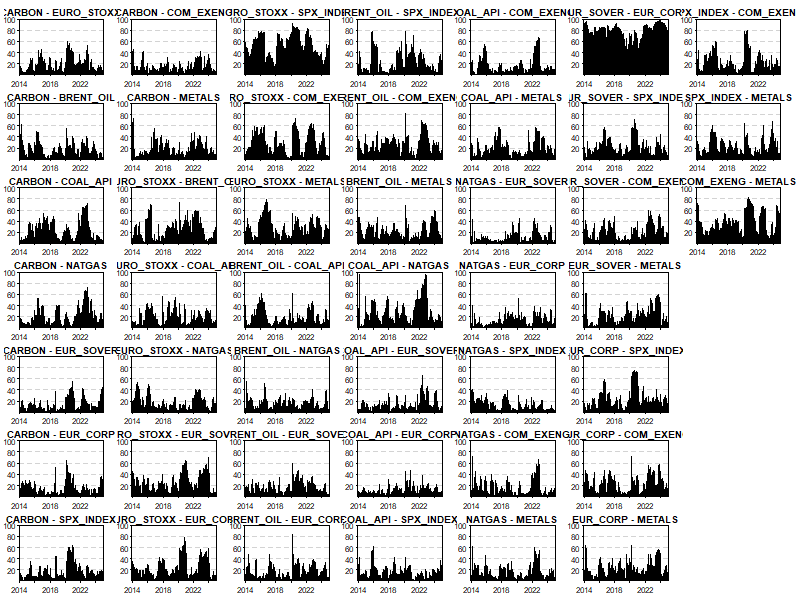
\includegraphics[width = 1.2\linewidth]{13bApdxD-10-220-VolPCI}
    \end{subfigure}
\end{figure}






\subsection{8-period forecast horizon and a rolling window of 180 observations}

\subsubsection{Static Return and Volatility Connectedness Matrix}

  \begin{table}[!ht]
    \caption{Static Return and Volatility Connectedness Matrix (Jan 2013 - Jan 2025)}
      \resizebox{\columnwidth}{!}{   
      \begin{tabular}{|l|l|l|l|l|l|l|l|l|l|l|l|}
      \multicolumn{12}{@{}l}{\em(a) Carbon returns connectedness matrix}\\ \hline
        ~ & CARBON & EUROSTOXX & BRENTOIL & COALAPI & NATGAS & EURSOVER & EURCORP & SPXINDEX & COMEXENG & METALS & FROM \\ \hline
        CARBON & 58.73 & 4.12 & 3.91 & 7.88 & 10.34 & 2.69 & 2.43 & 3.68 & 2.92 & 3.3 & 41.27 \\ \hline
        EUROSTOXX & 3.39 & 48.68 & 5.76 & 3.42 & 3.3 & 3.36 & 3.91 & 19.61 & 5.29 & 3.28 & 51.32 \\ \hline
        BRENTOIL & 3.7 & 6.12 & 56.35 & 5.5 & 3.71 & 2.85 & 2.46 & 7.32 & 8.25 & 3.74 & 43.65 \\ \hline
        COALAPI & 6.46 & 3.9 & 5.87 & 54.95 & 13.64 & 2.04 & 2.22 & 3.99 & 4.08 & 2.87 & 45.05 \\ \hline
        NATGAS & 10.06 & 3.2 & 4.03 & 13.38 & 57.41 & 2.03 & 1.95 & 2.71 & 2.77 & 2.45 & 42.59 \\ \hline
        EURSOVER & 2.21 & 3.22 & 2.9 & 1.85 & 1.87 & 47.39 & 31.45 & 2.41 & 2.25 & 4.43 & 52.61 \\ \hline
        EURCORP & 2.16 & 5.13 & 2.86 & 1.94 & 1.99 & 30.01 & 44.76 & 4.01 & 2.69 & 4.47 & 55.24 \\ \hline
        SPXINDEX & 2.58 & 17.81 & 6.93 & 3.46 & 2.26 & 2.47 & 2.89 & 52.51 & 6.38 & 2.71 & 47.49 \\ \hline
        COMEXENG & 2.66 & 5.13 & 7.45 & 3.6 & 2.65 & 2.37 & 2.51 & 6.56 & 52.2 & 14.86 & 47.8 \\ \hline
        METALS & 2.55 & 3.37 & 3.34 & 2.48 & 2.67 & 4.89 & 5.64 & 3.13 & 15.99 & 55.95 & 44.05 \\ \hline
        DST(TO) & 35.76 & 51.99 & 43.06 & 43.51 & 42.42 & 52.71 & 55.46 & 53.43 & 50.61 & 42.12 & 471.08 \\ \hline
        Inc. Own & 94.5 & 100.68 & 99.41 & 98.45 & 99.83 & 100.1 & 100.22 & 105.94 & 102.81 & 98.07 & cTCI/TCI \\ \hline
        NS (NET) & -5.5 & 0.68 & -0.59 & -1.55 & -0.17 & 0.1 & 0.22 & 5.94 & 2.81 & -1.93 & 52.34/47.11 \\ \hline
    \end{tabular}
    }
    \bigskip
      \resizebox{\columnwidth}{!}{
      \begin{tabular}{|l|l|l|l|l|l|l|l|l|l|l|l|}
    \multicolumn{12}{@{}l}{\em(b) Carbon volatility connectedness matrix}\\ \hline
        ~ & CARBON & EUROSTOXX & BRENTOIL & COALAPI & NATGAS & EURSOVER & EURCORP & SPXINDEX & COMEXENG & METALS & FROM \\ \hline
        CARBON & 57.54 & 4.29 & 4.24 & 6.61 & 7.04 & 3.68 & 3.29 & 4.63 & 3.58 & 5.1 & 42.46 \\ \hline
        EUROSTOXX & 3.64 & 47.92 & 5.2 & 3.73 & 3.31 & 5.24 & 4.1 & 16.18 & 4.86 & 5.81 & 52.08 \\ \hline
        BRENTOIL & 4.54 & 6.27 & 54.13 & 4.66 & 3.32 & 3.65 & 4.43 & 6.37 & 6.68 & 5.96 & 45.87 \\ \hline
        COALAPI & 4.31 & 5.16 & 4.37 & 59.14 & 7.71 & 3.82 & 2.8 & 4.58 & 3.16 & 4.95 & 40.86 \\ \hline
        NATGAS & 4.37 & 4.61 & 3.24 & 7.83 & 61.1 & 3.29 & 3.43 & 4.7 & 3.63 & 3.81 & 38.9 \\ \hline
        EURSOVER & 2.2 & 5.98 & 3.36 & 2.47 & 2.19 & 44.51 & 25.76 & 5.33 & 3.96 & 4.24 & 55.49 \\ \hline
        EURCORP & 2.95 & 5.35 & 2.3 & 2.49 & 2.54 & 28.14 & 42.31 & 5.81 & 4.68 & 3.43 & 57.69 \\ \hline
        SPXINDEX & 3.08 & 15.12 & 5.25 & 2.88 & 1.77 & 4.81 & 4.19 & 53.9 & 4.15 & 4.85 & 46.1 \\ \hline
        COMEXENG & 2.82 & 7.63 & 4.56 & 4.09 & 4.03 & 5.57 & 5.32 & 6.51 & 49.19 & 10.29 & 50.81 \\ \hline
        METALS & 3.96 & 7.74 & 4.37 & 3.92 & 3.82 & 5.1 & 6.4 & 6.17 & 9.52 & 49.01 & 50.99 \\ \hline
        DST(TO) & 31.86 & 62.14 & 36.9 & 38.68 & 35.72 & 63.29 & 59.73 & 60.27 & 44.22 & 48.44 & 481.25 \\ \hline
        Inc. Own & 89.41 & 110.06 & 91.03 & 97.82 & 96.83 & 107.8 & 102.03 & 114.17 & 93.41 & 97.45 & cTCI/TCI \\ \hline
        NS (NET) & -10.59 & 10.06 & -8.97 & -2.18 & -3.17 & 7.8 & 2.03 & 14.17 & -6.59 & -2.55 & 53.47/48.12 \\ \hline
    \end{tabular}
    }
\end{table}




\subsubsection{Dynamic Return and Volatility Net Directional Connectedness}

\begin{figure}[H]
  \caption{Dynamic Net Directional Connectedness (Jan 2013 – Jan 2025)}
    \centering
      \begin{subfigure}[a]{\textwidth}
        \caption{Dynamic return net directional connectedness}
        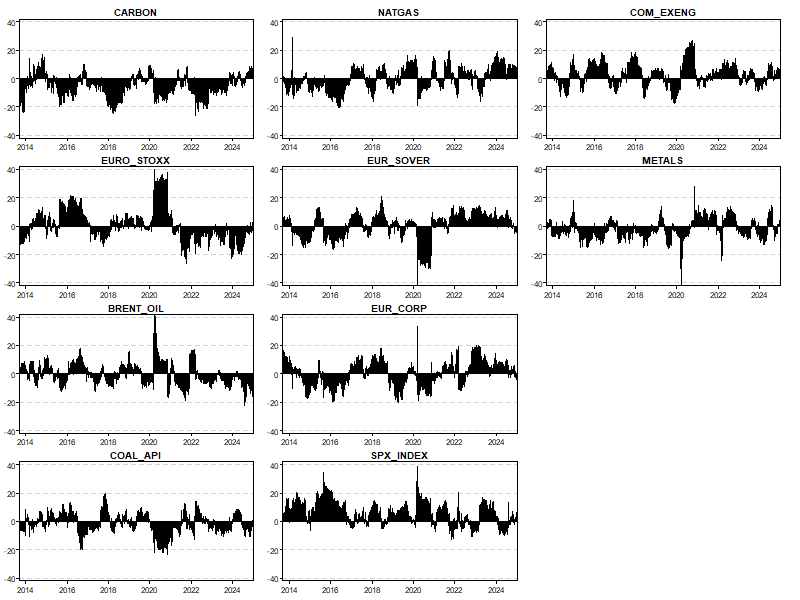
\includegraphics[width = 1.25\linewidth]{14aApdxD-8-180-RetNDC}
      \end{subfigure}
\end{figure}
\begin{figure}[H]
  \ContinuedFloat
  \centering
      \begin{subfigure}[b]{\textwidth}
        \caption{Dynamic volatility net directional connectedness}
        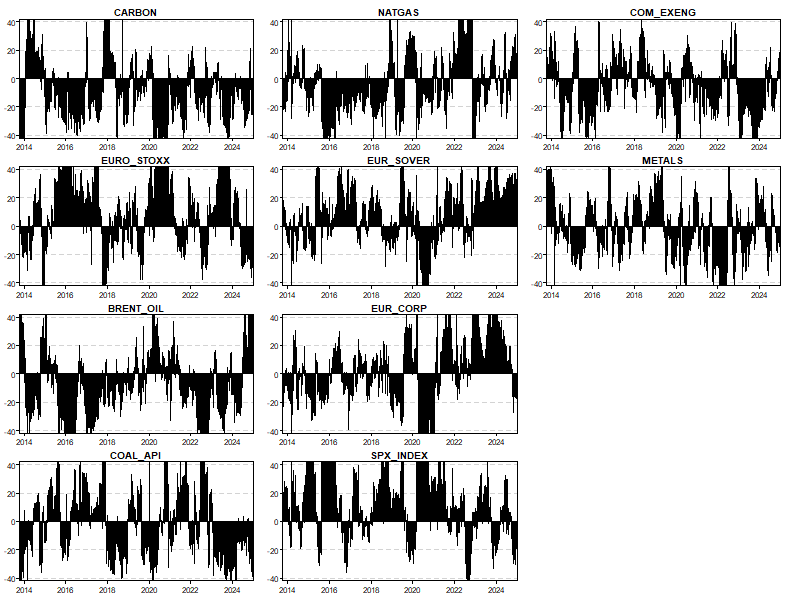
\includegraphics[width = 1.25\linewidth]{14bApdxD-8-180-VolNDC}
      \end{subfigure}
\end{figure}



\subsubsection{Static Return and Volatility Pairwise Directional Connectedness}

\begin{figure}[!ht]
  \caption{Network Representation of Pairwise Connectedness Index (Jan 2013 – Jan 2025)}
  \begin{minipage}{.8\textwidth}
    \subfloat[Static Return PCI network]{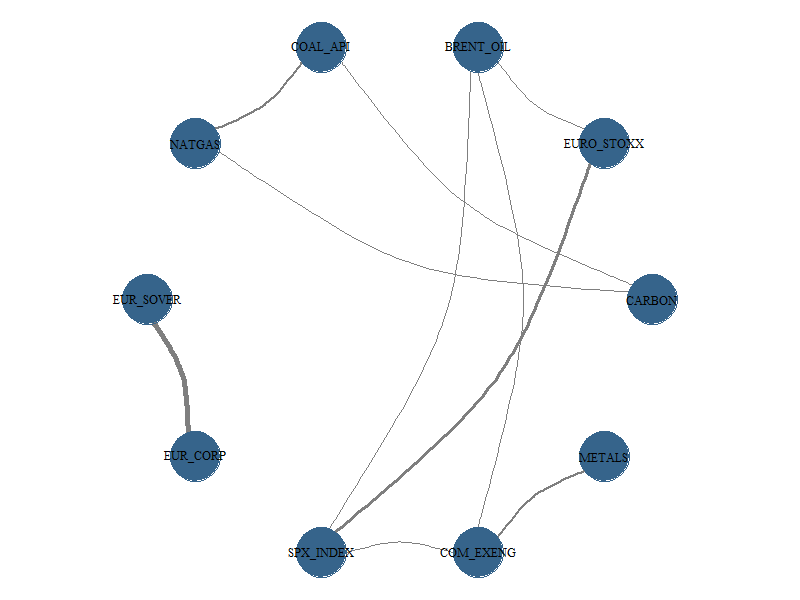
\includegraphics[width = \linewidth]{15aApdxD-8-180-RetNtwrk}}
  \end{minipage}
  \hfill
  \begin{minipage}{.8\textwidth}
    \subfloat[Static Volatility PCI network]{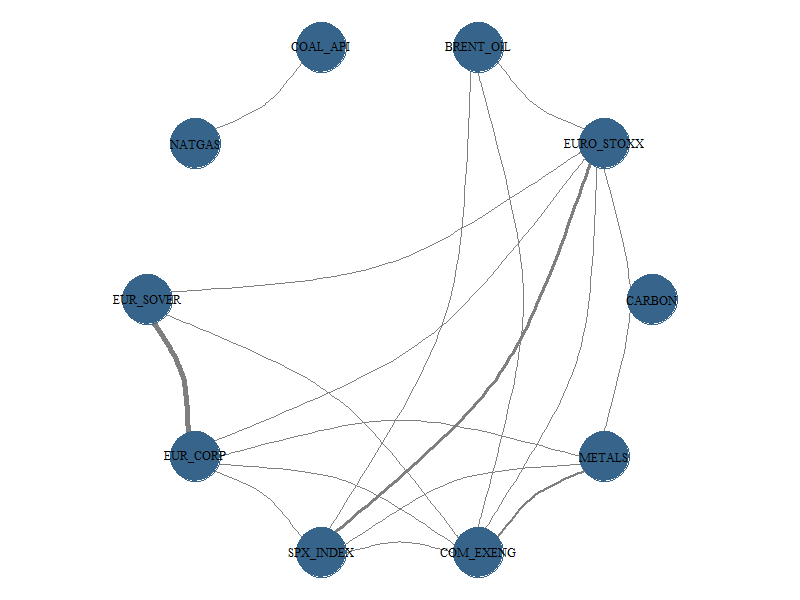
\includegraphics[width = \linewidth]{15bApdxD-8-180-VolNtwrk}}
  \end{minipage}
\end{figure}



\newpage

\subsubsection{Dynamic Return and Volatility Pairwise Directional Connectedness}

\begin{figure}[!ht]
  \caption{Dynamic Return and Volatility Pairwise Connectedness Index (Jan 2013 – Jan 2025)}
  \centering
  \begin{subfigure}[a]{\textwidth}
    \caption{Dynamic return PCI}
    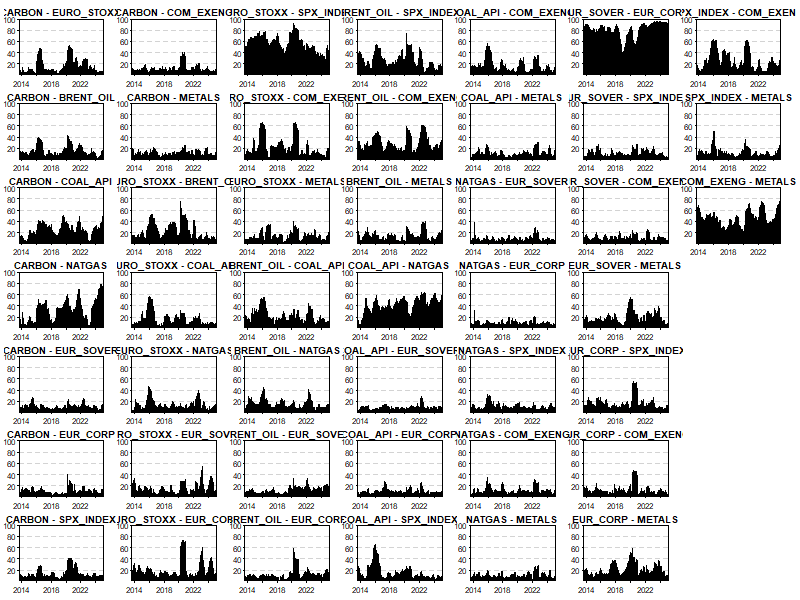
\includegraphics[width = 1.1\linewidth]{16aApdxD-8-180-RetPCI}
  \end{subfigure}
\end{figure}
\begin{figure}[!ht]
  \ContinuedFloat
  \centering
    \begin{subfigure}[b]{\textwidth}\ContinuedFloat
      \caption{Dynamic volatility PCI}
      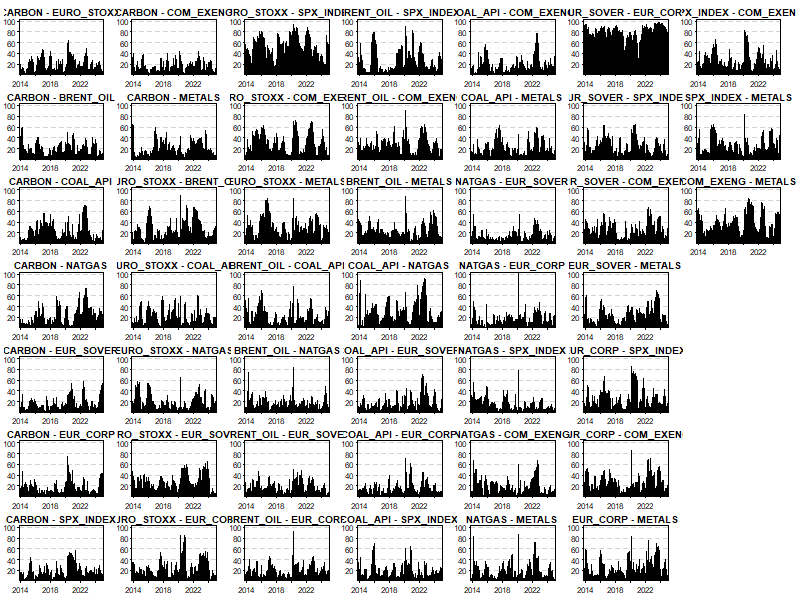
\includegraphics[width = 1.2\linewidth]{16bApdxD-8-180-VolPCI}
    \end{subfigure}
\end{figure}









\subsection{8-period forecast horizon and a rolling window of 200 observations}

\subsubsection{Static Return and Volatility Connectedness Matrix}

  \begin{table}[!ht]
    \caption{Static Return and Volatility Connectedness Matrix (Jan 2013 - Jan 2025)}
      \resizebox{\columnwidth}{!}{
      \begin{tabular}{|l|l|l|l|l|l|l|l|l|l|l|l|}
    \multicolumn{12}{@{}l}{\em(a) Carbon returns connectedness matrix}\\ \hline
        ~ & CARBON & EUROSTOXX & BRENTOIL & COALAPI & NATGAS & EURSOVER & EURCORP & SPXINDEX & COMEXENG & METALS & FROM \\ \hline
        CARBON & 60.33 & 3.99 & 3.77 & 7.83 & 10.23 & 2.42 & 2.21 & 3.44 & 2.72 & 3.05 & 39.67 \\ \hline
        EUROSTOXX & 3.26 & 49.92 & 5.7 & 3.3 & 3.08 & 3.01 & 3.64 & 19.93 & 5.19 & 2.98 & 50.08 \\ \hline
        BRENTOIL & 3.47 & 5.98 & 57.62 & 5.41 & 3.57 & 2.65 & 2.3 & 7.25 & 8.28 & 3.46 & 42.38 \\ \hline
        COALAPI & 6.33 & 3.75 & 5.78 & 56.18 & 13.78 & 1.83 & 2.01 & 3.82 & 3.94 & 2.59 & 43.82 \\ \hline
        NATGAS & 9.94 & 3 & 3.86 & 13.6 & 58.93 & 1.78 & 1.72 & 2.44 & 2.52 & 2.21 & 41.07 \\ \hline
        EURSOVER & 1.99 & 2.97 & 2.64 & 1.64 & 1.63 & 48.54 & 32.01 & 2.25 & 2 & 4.33 & 51.46 \\ \hline
        EURCORP & 1.94 & 5.03 & 2.68 & 1.71 & 1.75 & 30.44 & 45.63 & 3.94 & 2.53 & 4.33 & 54.37 \\ \hline
        SPXINDEX & 2.38 & 17.98 & 6.82 & 3.32 & 2 & 2.25 & 2.7 & 53.68 & 6.39 & 2.47 & 46.32 \\ \hline
        COMEXENG & 2.47 & 5.04 & 7.42 & 3.46 & 2.38 & 2.12 & 2.33 & 6.56 & 53.26 & 14.96 & 46.74 \\ \hline
        METALS & 2.34 & 3.1 & 3.07 & 2.25 & 2.42 & 4.81 & 5.56 & 2.9 & 16.18 & 57.37 & 42.63 \\ \hline
        DST(TO) & 34.12 & 50.84 & 41.75 & 42.53 & 40.82 & 51.31 & 54.49 & 52.53 & 49.76 & 40.39 & 458.54 \\ \hline
        Inc. Own & 94.45 & 100.75 & 99.37 & 98.71 & 99.76 & 99.85 & 100.12 & 106.21 & 103.02 & 97.76 & cTCI/TCI \\ \hline
        NS (NET) & -5.55 & 0.75 & -0.63 & -1.29 & -0.24 & -0.15 & 0.12 & 6.21 & 3.02 & -2.24 & 50.95/45.85 \\ \hline
    \end{tabular}
    }
    \bigskip
      \resizebox{\columnwidth}{!}{
      \begin{tabular}{|l|l|l|l|l|l|l|l|l|l|l|l|}
    \multicolumn{12}{@{}l}{\em(b) Carbon volatility connectedness matrix}\\ \hline
        ~ & CARBON & EUROSTOXX & BRENTOIL & COALAPI & NATGAS & EURSOVER & EURCORP & SPXINDEX & COMEXENG & METALS & FROM \\ \hline
        CARBON & 60.17 & 4.17 & 3.78 & 6.68 & 6.57 & 3.32 & 3.11 & 4.33 & 3.26 & 4.61 & 39.83 \\ \hline
        EUROSTOXX & 3.29 & 49.69 & 5.1 & 3.09 & 2.94 & 4.86 & 3.93 & 16.76 & 4.8 & 5.55 & 50.31 \\ \hline
        BRENTOIL & 4.03 & 6.12 & 56.72 & 4.48 & 3.04 & 3.25 & 4.01 & 6.11 & 6.72 & 5.54 & 43.28 \\ \hline
        COALAPI & 4.14 & 4.95 & 3.92 & 62.24 & 7.35 & 3.39 & 2.39 & 4.07 & 2.83 & 4.7 & 37.76 \\ \hline
        NATGAS & 4.18 & 4.25 & 2.96 & 7.77 & 63.79 & 2.87 & 3.22 & 4.26 & 3.21 & 3.49 & 36.21 \\ \hline
        EURSOVER & 1.94 & 5.82 & 3.08 & 2.1 & 1.74 & 46.3 & 26.28 & 5.1 & 3.44 & 4.21 & 53.7 \\ \hline
        EURCORP & 2.58 & 5.27 & 2.19 & 2.05 & 2.04 & 28.8 & 44.04 & 5.7 & 4.16 & 3.17 & 55.96 \\ \hline
        SPXINDEX & 2.84 & 15.41 & 4.97 & 2.56 & 1.49 & 4.35 & 3.82 & 56.19 & 3.92 & 4.45 & 43.81 \\ \hline
        COMEXENG & 2.32 & 7.68 & 4.52 & 3.73 & 3.57 & 4.87 & 4.97 & 6.12 & 51.84 & 10.37 & 48.16 \\ \hline
        METALS & 3.62 & 7.62 & 4.07 & 3.51 & 3.33 & 4.94 & 5.95 & 5.62 & 9.94 & 51.42 & 48.58 \\ \hline
        DST(TO) & 28.93 & 61.29 & 34.59 & 35.97 & 32.07 & 60.65 & 57.69 & 58.07 & 42.27 & 46.09 & 457.61 \\ \hline
        Inc. Own & 89.1 & 110.98 & 91.3 & 98.21 & 95.85 & 106.95 & 101.73 & 114.26 & 94.11 & 97.51 & cTCI/TCI \\ \hline
        NS (NET) & -10.9 & 10.98 & -8.7 & -1.79 & -4.15 & 6.95 & 1.73 & 14.26 & -5.89 & -2.49 & 50.85/45.76 \\ \hline
    \end{tabular}
    }
\end{table}




\subsubsection{Dynamic Return and Volatility Net Directional Connectedness}

\begin{figure}[H]
  \caption{Dynamic Net Directional Connectedness (Jan 2013 – Jan 2025)}
    \centering
      \begin{subfigure}[a]{\textwidth}
        \caption{Dynamic return net directional connectedness}
        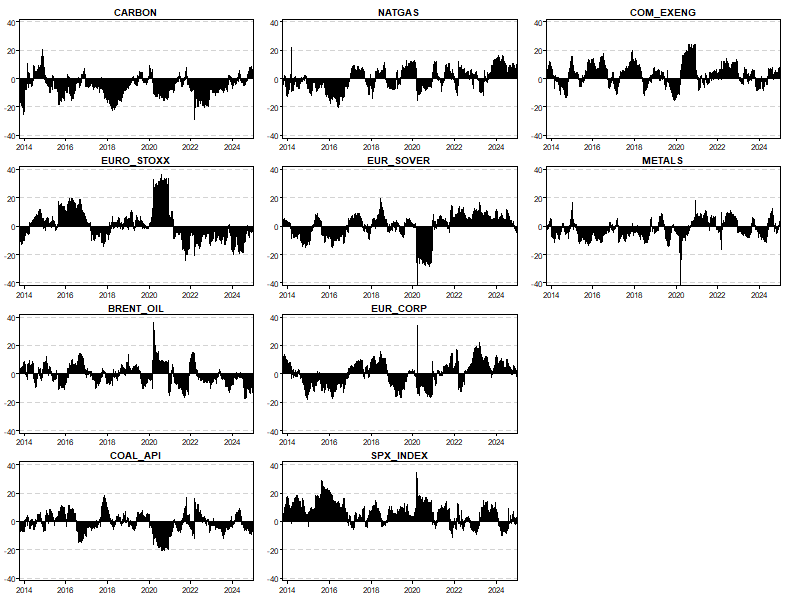
\includegraphics[width = 1.25\linewidth]{17aApdxD-8-200-RetNDC}
      \end{subfigure}
\end{figure}
\begin{figure}[H]
  \ContinuedFloat
  \centering
      \begin{subfigure}[b]{\textwidth}
        \caption{Dynamic volatility net directional connectedness}
        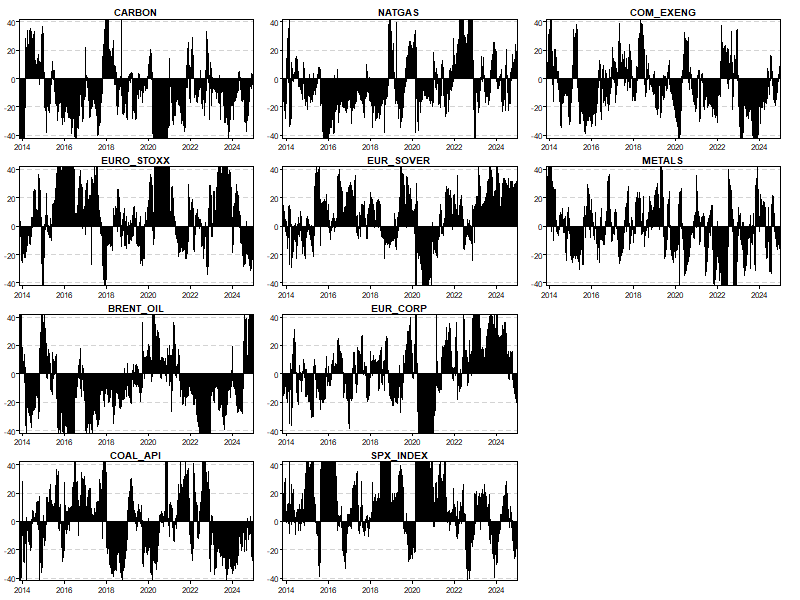
\includegraphics[width = 1.25\linewidth]{17bApdxD-8-200-VolNDC}
      \end{subfigure}
\end{figure}



\subsubsection{Static Return and Volatility Pairwise Directional Connectedness}

\begin{figure}[!ht]
  \caption{Network Representation of Pairwise Connectedness Index (Jan 2013 – Jan 2025)}
  \begin{minipage}{.8\textwidth}
    \subfloat[Static Return PCI network]{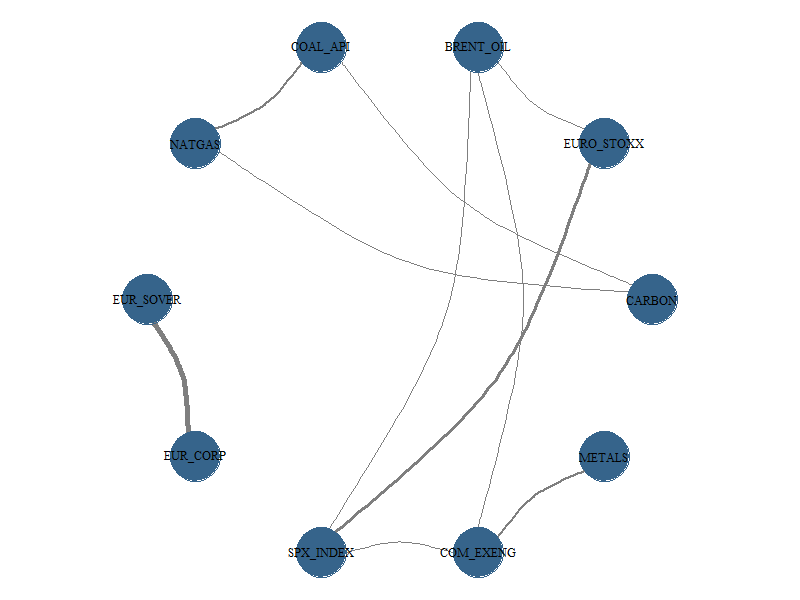
\includegraphics[width = \linewidth]{18aApdxD-8-200-RetNtwrk}}
  \end{minipage}
  \hfill
  \begin{minipage}{.8\textwidth}
    \subfloat[Static Volatility PCI network]{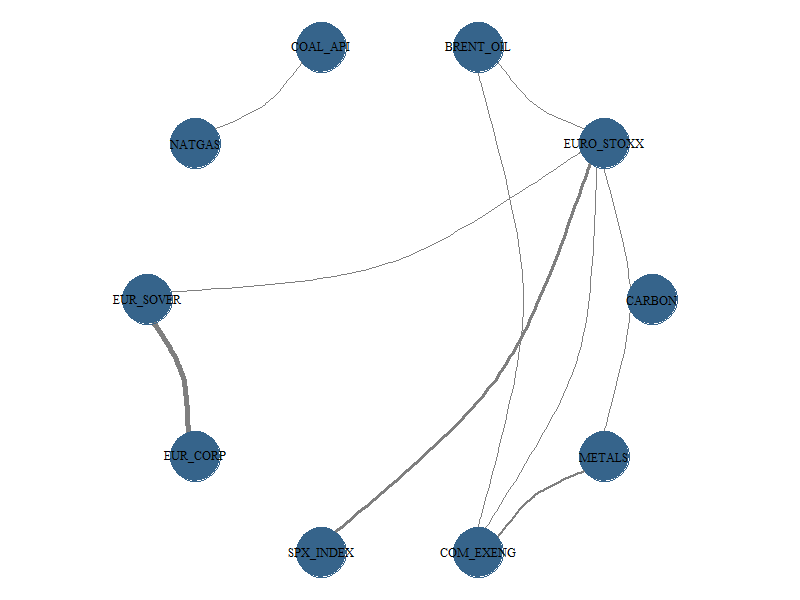
\includegraphics[width = \linewidth]{18bApdxD-8-200-VolNtwrk}}
  \end{minipage}
\end{figure}



\newpage

\subsubsection{Dynamic Return and Volatility Pairwise Directional Connectedness}

\begin{figure}[!ht]
  \caption{Dynamic Return and Volatility Pairwise Connectedness Index (Jan 2013 – Jan 2025)}
  \centering
  \begin{subfigure}[a]{\textwidth}
    \caption{Dynamic return PCI}
    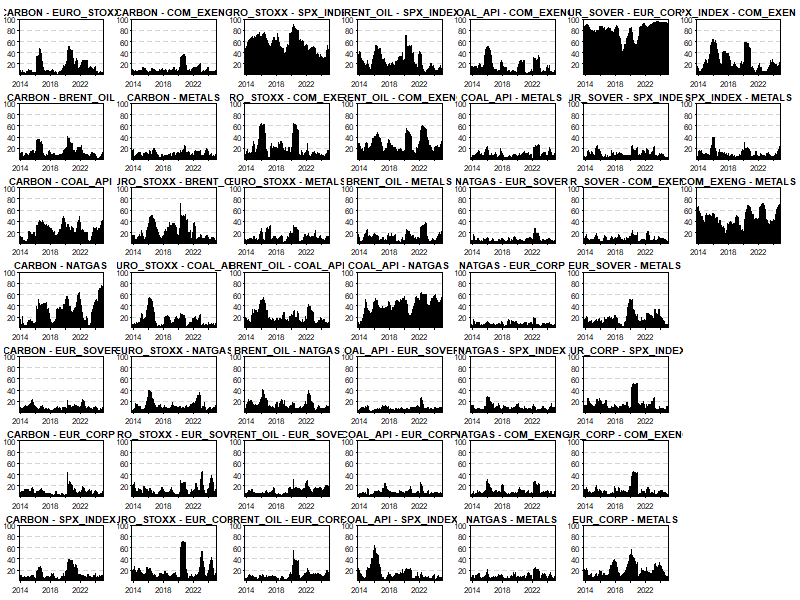
\includegraphics[width = 1.1\linewidth]{19aApdxD-8-200-RetPCI}
  \end{subfigure}
\end{figure}
\begin{figure}[!ht]
  \ContinuedFloat
  \centering
    \begin{subfigure}[b]{\textwidth}\ContinuedFloat
      \caption{Dynamic volatility PCI}
      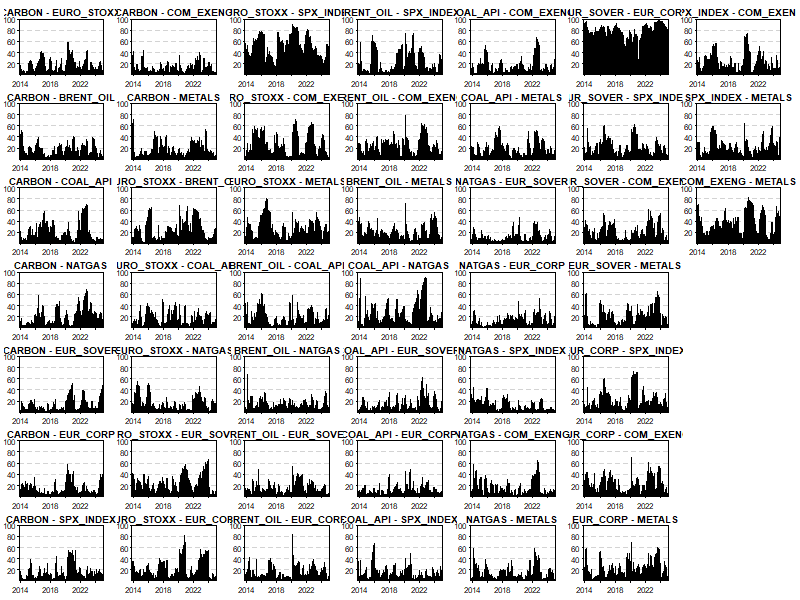
\includegraphics[width = 1.2\linewidth]{19bApdxD-8-200-VolPCI}
    \end{subfigure}
\end{figure}








\subsection{8-period forecast horizon and a rolling window of 220 observations}

\subsubsection{Static Return and Volatility Connectedness Matrix}

  \begin{table}[!ht]
    \caption{Static Return and Volatility Connectedness Matrix (Jan 2013 - Jan 2025)}
      \resizebox{\columnwidth}{!}{
      \begin{tabular}{|l|l|l|l|l|l|l|l|l|l|l|l|}
    \multicolumn{12}{@{}l}{\em(a) Carbon returns connectedness matrix}\\ \hline
        ~ & CARBON & EUROSTOXX & BRENTOIL & COALAPI & NATGAS & EURSOVER & EURCORP & SPXINDEX & COMEXENG & METALS & FROM \\ \hline
        CARBON & 61.59 & 3.93 & 3.64 & 7.76 & 10.08 & 2.24 & 2.07 & 3.26 & 2.57 & 2.86 & 38.41 \\ \hline
        EUROSTOXX & 3.15 & 50.93 & 5.67 & 3.2 & 2.9 & 2.71 & 3.41 & 20.17 & 5.13 & 2.73 & 49.07 \\ \hline
        BRENTOIL & 3.3 & 5.9 & 58.62 & 5.37 & 3.45 & 2.48 & 2.19 & 7.17 & 8.31 & 3.22 & 41.38 \\ \hline
        COALAPI & 6.2 & 3.63 & 5.73 & 57.17 & 13.87 & 1.69 & 1.86 & 3.68 & 3.8 & 2.36 & 42.83 \\ \hline
        NATGAS & 9.8 & 2.83 & 3.73 & 13.77 & 60.14 & 1.6 & 1.57 & 2.19 & 2.34 & 2.03 & 39.86 \\ \hline
        EURSOVER & 1.83 & 2.76 & 2.44 & 1.47 & 1.43 & 49.48 & 32.44 & 2.12 & 1.8 & 4.23 & 50.52 \\ \hline
        EURCORP & 1.81 & 4.98 & 2.57 & 1.53 & 1.55 & 30.74 & 46.27 & 3.9 & 2.43 & 4.21 & 53.73 \\ \hline
        SPXINDEX & 2.22 & 18.15 & 6.71 & 3.18 & 1.78 & 2.07 & 2.56 & 54.62 & 6.44 & 2.26 & 45.38 \\ \hline
        COMEXENG & 2.31 & 4.99 & 7.41 & 3.32 & 2.15 & 1.93 & 2.17 & 6.6 & 54.09 & 15.02 & 45.91 \\ \hline
        METALS & 2.19 & 2.85 & 2.84 & 2.05 & 2.2 & 4.76 & 5.48 & 2.69 & 16.34 & 58.6 & 41.4 \\ \hline
        DST(TO) & 32.81 & 50.03 & 40.74 & 41.65 & 39.42 & 50.23 & 53.75 & 51.77 & 49.15 & 38.94 & 448.48 \\ \hline
        Inc. Own & 94.4 & 100.96 & 99.36 & 98.83 & 99.56 & 99.71 & 100.02 & 106.39 & 103.24 & 97.54 & cTCI/TCI \\ \hline
        NS (NET) & -5.6 & 0.96 & -0.64 & -1.17 & -0.44 & -0.29 & 0.02 & 6.39 & 3.24 & -2.46 & 49.83/44.85 \\ \hline
    \end{tabular}
    }
    \bigskip
      \resizebox{\columnwidth}{!}{
      \begin{tabular}{|l|l|l|l|l|l|l|l|l|l|l|l|}
    \multicolumn{12}{@{}l}{\em(b) Carbon volatility connectedness matrix}\\ \hline
        ~ & CARBON & EUROSTOXX & BRENTOIL & COALAPI & NATGAS & EURSOVER & EURCORP & SPXINDEX & COMEXENG & METALS & FROM \\ \hline
        CARBON & 62.2 & 4.14 & 3.49 & 6.68 & 6.23 & 3.06 & 2.83 & 4.04 & 3.14 & 4.2 & 37.8 \\ \hline
        EUROSTOXX & 2.95 & 50.86 & 4.93 & 2.73 & 2.66 & 4.69 & 3.87 & 17.15 & 4.84 & 5.33 & 49.14 \\ \hline
        BRENTOIL & 3.56 & 6.04 & 58.65 & 4.31 & 2.84 & 2.92 & 3.59 & 5.91 & 6.93 & 5.24 & 41.35 \\ \hline
        COALAPI & 4.12 & 4.62 & 3.28 & 64.8 & 7 & 3.13 & 2.22 & 3.66 & 2.66 & 4.52 & 35.2 \\ \hline
        NATGAS & 4.07 & 3.96 & 2.61 & 7.59 & 66.13 & 2.57 & 3.05 & 3.93 & 2.92 & 3.16 & 33.87 \\ \hline
        EURSOVER & 1.71 & 5.66 & 2.88 & 1.82 & 1.5 & 47.64 & 26.63 & 4.99 & 3.08 & 4.09 & 52.36 \\ \hline
        EURCORP & 2.3 & 5.25 & 2.14 & 1.71 & 1.66 & 29.27 & 45.3 & 5.68 & 3.66 & 3.02 & 54.7 \\ \hline
        SPXINDEX & 2.61 & 15.47 & 4.61 & 2.36 & 1.32 & 4.01 & 3.62 & 58.11 & 3.72 & 4.17 & 41.89 \\ \hline
        COMEXENG & 1.91 & 7.65 & 4.54 & 3.52 & 3.19 & 4.42 & 4.56 & 5.92 & 53.86 & 10.43 & 46.14 \\ \hline
        METALS & 3.41 & 7.37 & 3.76 & 3.24 & 2.95 & 4.79 & 5.5 & 5.17 & 10.24 & 53.57 & 46.43 \\ \hline
        DST(TO) & 26.64 & 60.17 & 32.23 & 33.96 & 29.35 & 58.88 & 55.87 & 56.45 & 41.18 & 44.17 & 438.89 \\ \hline
        Inc. Own & 88.84 & 111.02 & 90.88 & 98.75 & 95.49 & 106.52 & 101.17 & 114.56 & 95.04 & 97.73 & cTCI/TCI \\ \hline
        NS (NET) & -11.16 & 11.02 & -9.12 & -1.25 & -4.51 & 6.52 & 1.17 & 14.56 & -4.96 & -2.27 & 48.77/43.89 \\ \hline
    \end{tabular}
    }
\end{table}




\subsubsection{Dynamic Return and Volatility Net Directional Connectedness}

\begin{figure}[H]
  \caption{Dynamic Net Directional Connectedness (Jan 2013 – Jan 2025)}
    \centering
      \begin{subfigure}[a]{\textwidth}
        \caption{Dynamic return net directional connectedness}
        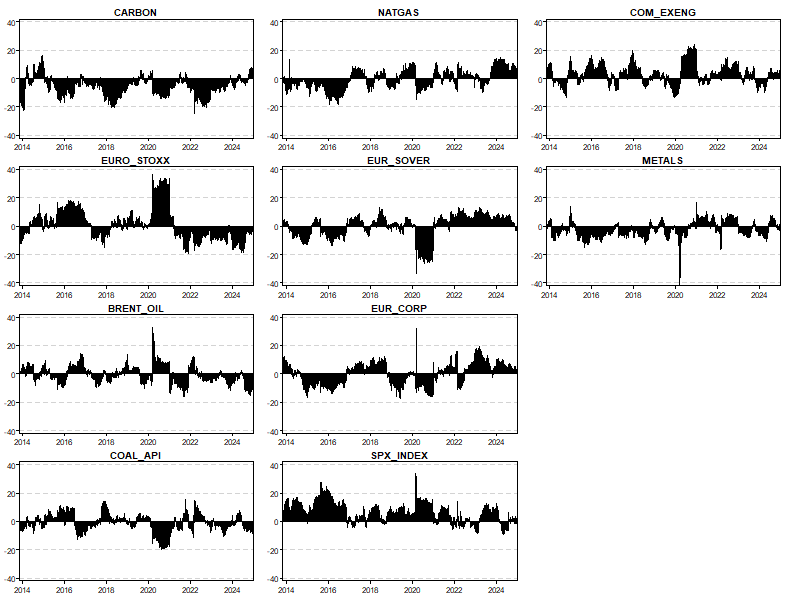
\includegraphics[width = 1.25\linewidth]{20aApdxD-8-220-RetNDC}
      \end{subfigure}
\end{figure}
\begin{figure}[H]
  \ContinuedFloat
  \centering
      \begin{subfigure}[b]{\textwidth}
        \caption{Dynamic volatility net directional connectedness}
        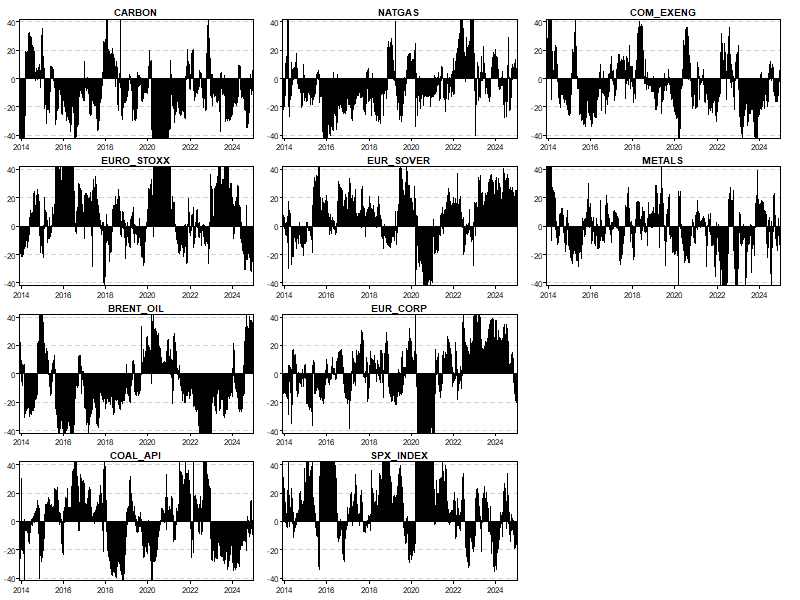
\includegraphics[width = 1.25\linewidth]{20bApdxD-8-220-VolNDC}
      \end{subfigure}
\end{figure}



\subsubsection{Static Return and Volatility Pairwise Directional Connectedness}

\begin{figure}[!ht]
  \caption{Network Representation of Pairwise Connectedness Index (Jan 2013 – Jan 2025)}
  \begin{minipage}{.8\textwidth}
    \subfloat[Static Return PCI network]{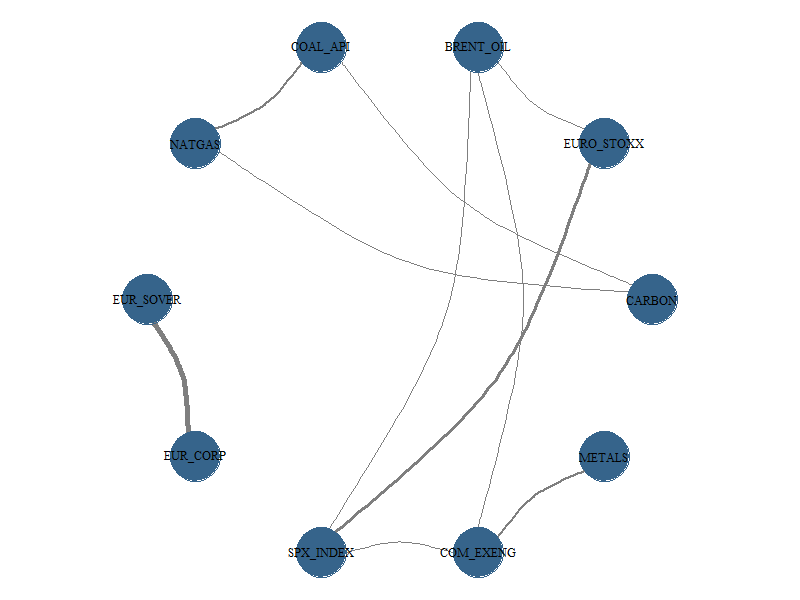
\includegraphics[width = \linewidth]{21aApdxD-8-220-RetNtwrk}}
  \end{minipage}
  \hfill
  \begin{minipage}{.8\textwidth}
    \subfloat[Static Volatility PCI network]{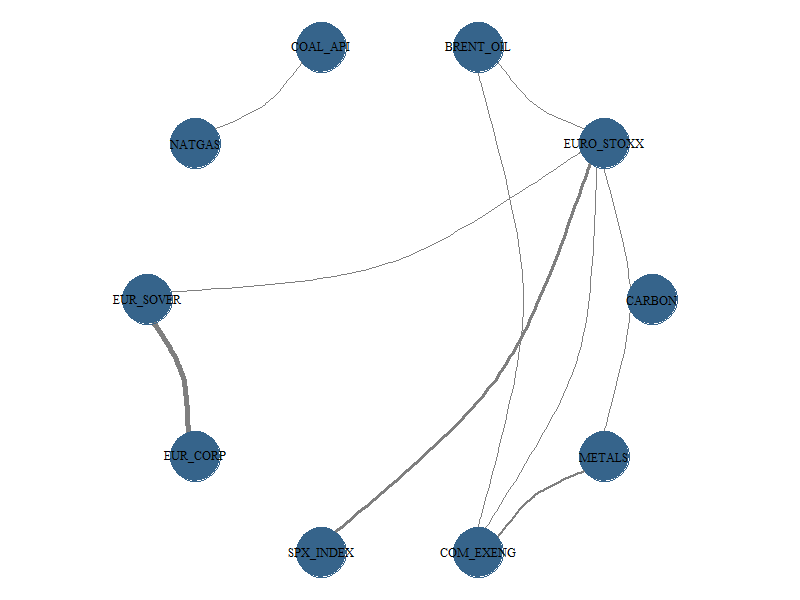
\includegraphics[width = \linewidth]{21bApdxD-8-220-VolNtwrk}}
  \end{minipage}
\end{figure}



\newpage

\subsubsection{Dynamic Return and Volatility Pairwise Directional Connectedness}

\begin{figure}[!ht]
  \caption{Dynamic Return and Volatility Pairwise Connectedness Index (Jan 2013 – Jan 2025)}
  \centering
  \begin{subfigure}[a]{\textwidth}
    \caption{Dynamic return PCI}
    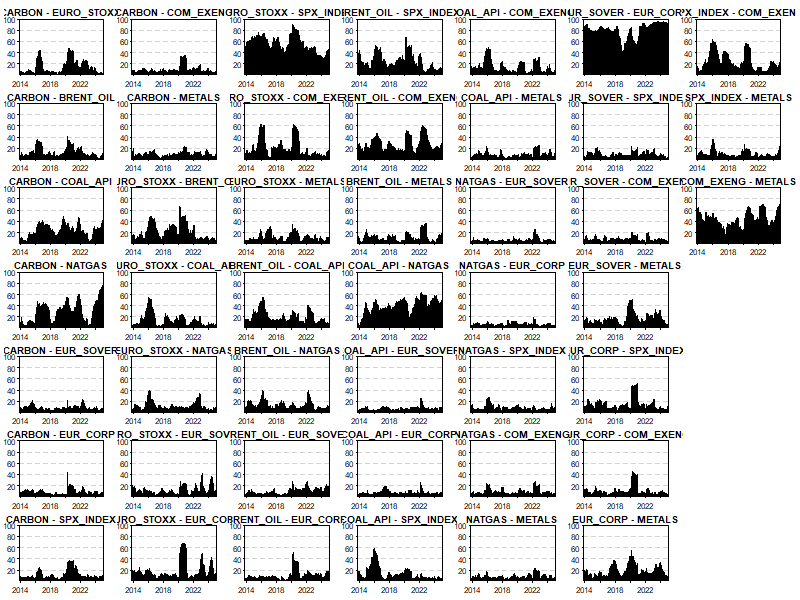
\includegraphics[width = 1.1\linewidth]{22aApdxD-8-220-RetPCI}
  \end{subfigure}
\end{figure}
\begin{figure}[!ht]
  \ContinuedFloat
  \centering
    \begin{subfigure}[b]{\textwidth}\ContinuedFloat
      \caption{Dynamic volatility PCI}
      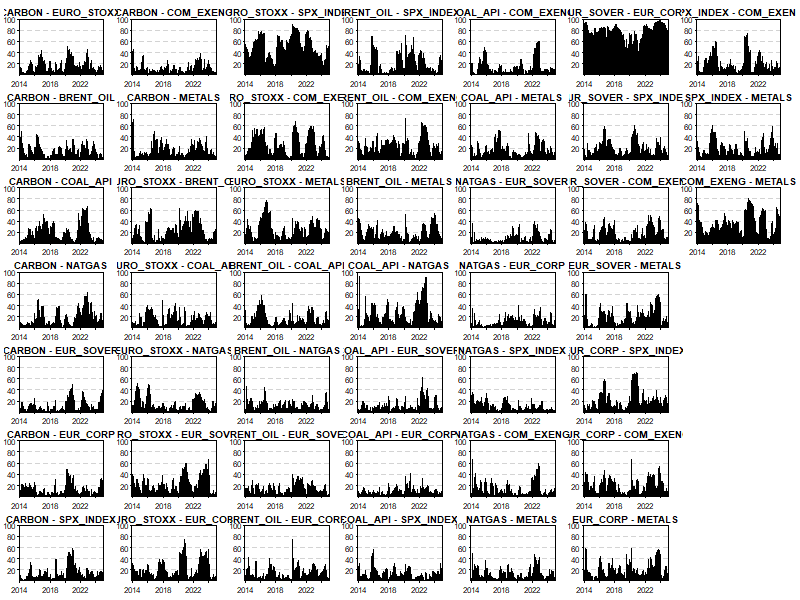
\includegraphics[width = 1.2\linewidth]{22bApdxD-8-220-VolPCI}
    \end{subfigure}
\end{figure}










\subsection{12-period forecast horizon and a rolling window of 180 observations}

\subsubsection{Static Return and Volatility Connectedness Matrix}

  \begin{table}[!ht]
    \caption{Static Return and Volatility Connectedness Matrix (Jan 2013 - Jan 2025)}
      \resizebox{\columnwidth}{!}{
      \begin{tabular}{|l|l|l|l|l|l|l|l|l|l|l|l|}
    \multicolumn{12}{@{}l}{\em(a) Carbon returns connectedness matrix}\\ \hline
        ~ & CARBON & EUROSTOXX & BRENTOIL & COALAPI & NATGAS & EURSOVER & EURCORP & SPXINDEX & COMEXENG & METALS & FROM \\ \hline
        CARBON & 58.33 & 4.13 & 3.97 & 7.9 & 10.32 & 2.77 & 2.5 & 3.72 & 2.98 & 3.39 & 41.67 \\ \hline
        EUROSTOXX & 3.43 & 48.44 & 5.78 & 3.45 & 3.36 & 3.41 & 3.95 & 19.53 & 5.31 & 3.33 & 51.56 \\ \hline
        BRENTOIL & 3.74 & 6.15 & 55.99 & 5.54 & 3.77 & 2.9 & 2.52 & 7.35 & 8.26 & 3.79 & 44.01 \\ \hline
        COALAPI & 6.48 & 3.93 & 5.89 & 54.66 & 13.62 & 2.09 & 2.26 & 4.03 & 4.12 & 2.93 & 45.34 \\ \hline
        NATGAS & 10.05 & 3.25 & 4.07 & 13.36 & 57.07 & 2.08 & 2.01 & 2.78 & 2.84 & 2.5 & 42.93 \\ \hline
        EURSOVER & 2.27 & 3.27 & 2.96 & 1.9 & 1.95 & 47.08 & 31.3 & 2.47 & 2.32 & 4.48 & 52.92 \\ \hline
        EURCORP & 2.19 & 5.15 & 2.91 & 1.99 & 2.07 & 29.9 & 44.54 & 4.04 & 2.71 & 4.5 & 55.46 \\ \hline
        SPXINDEX & 2.63 & 17.76 & 6.94 & 3.51 & 2.3 & 2.54 & 2.93 & 52.24 & 6.4 & 2.76 & 47.76 \\ \hline
        COMEXENG & 2.69 & 5.18 & 7.48 & 3.64 & 2.69 & 2.43 & 2.57 & 6.6 & 51.91 & 14.81 & 48.09 \\ \hline
        METALS & 2.58 & 3.45 & 3.41 & 2.53 & 2.74 & 4.92 & 5.68 & 3.22 & 15.92 & 55.54 & 44.46 \\ \hline
        DST(TO) & 36.06 & 52.28 & 43.39 & 43.82 & 42.82 & 53.03 & 55.73 & 53.74 & 50.85 & 42.49 & 474.2 \\ \hline
        Inc. Own & 94.39 & 100.72 & 99.38 & 98.47 & 99.89 & 100.11 & 100.27 & 105.98 & 102.76 & 98.03 & cTCI/TCI \\ \hline
        NS (NET) & -5.61 & 0.72 & -0.62 & -1.53 & -0.11 & 0.11 & 0.27 & 5.98 & 2.76 & -1.97 & 52.69/47.42 \\ \hline
    \end{tabular}
    }
    \bigskip
      \resizebox{\columnwidth}{!}{
    \begin{tabular}{|l|l|l|l|l|l|l|l|l|l|l|l|}
    \multicolumn{12}{@{}l}{\em(b) Carbon volatility connectedness matrix}\\ \hline
        ~ & CARBON & EUROSTOXX & BRENTOIL & COALAPI & NATGAS & EURSOVER & EURCORP & SPXINDEX & COMEXENG & METALS & FROM \\ \hline
        CARBON & 49.07 & 5.05 & 5.04 & 7.53 & 8.1 & 4.71 & 4.25 & 6.24 & 4.55 & 5.47 & 50.93 \\ \hline
        EUROSTOXX & 4.34 & 42.48 & 5.5 & 4.66 & 4.47 & 5.91 & 4.68 & 15.49 & 5.76 & 6.72 & 57.52 \\ \hline
        BRENTOIL & 4.91 & 7.05 & 46.16 & 5.52 & 4.3 & 4.89 & 5.5 & 7.04 & 7.5 & 7.13 & 53.84 \\ \hline
        COALAPI & 5.42 & 6.83 & 4.96 & 50.79 & 8.67 & 4.61 & 3.48 & 5.51 & 3.82 & 5.91 & 49.21 \\ \hline
        NATGAS & 5.12 & 5.38 & 4.23 & 8.78 & 52.69 & 4.47 & 4.44 & 5.78 & 4.38 & 4.72 & 47.31 \\ \hline
        EURSOVER & 2.74 & 6.84 & 3.83 & 3.16 & 2.59 & 41.18 & 23.89 & 6.2 & 4.83 & 4.75 & 58.82 \\ \hline
        EURCORP & 3.51 & 6.06 & 2.89 & 3.07 & 3.37 & 26.97 & 38.08 & 6.43 & 5.71 & 3.9 & 61.92 \\ \hline
        SPXINDEX & 4 & 14.79 & 5.55 & 3.89 & 2.41 & 5.65 & 4.67 & 47.45 & 5.22 & 6.37 & 52.55 \\ \hline
        COMEXENG & 3.54 & 8.03 & 4.9 & 4.53 & 4.92 & 6.48 & 6.13 & 7.47 & 44.23 & 9.77 & 55.77 \\ \hline
        METALS & 4.45 & 8.84 & 5.11 & 4.64 & 4.75 & 5.52 & 7.13 & 7.41 & 9.82 & 42.32 & 57.68 \\ \hline
        DST(TO) & 38.03 & 68.87 & 42.02 & 45.78 & 43.58 & 69.22 & 64.17 & 67.57 & 51.57 & 54.74 & 545.55 \\ \hline
        Inc. Own & 87.1 & 111.35 & 88.18 & 96.57 & 96.27 & 110.4 & 102.26 & 115.01 & 95.8 & 97.06 & cTCI/TCI \\ \hline
        NS (NET) & -12.9 & 11.35 & -11.82 & -3.43 & -3.73 & 10.4 & 2.26 & 15.01 & -4.2 & -2.94 & 60.62/54.55 \\ \hline
    \end{tabular}
    }
\end{table}




\subsubsection{Dynamic Return and Volatility Net Directional Connectedness}

\begin{figure}[H]
  \caption{Dynamic Net Directional Connectedness (Jan 2013 – Jan 2025)}
    \centering
      \begin{subfigure}[a]{\textwidth}
        \caption{Dynamic return net directional connectedness}
        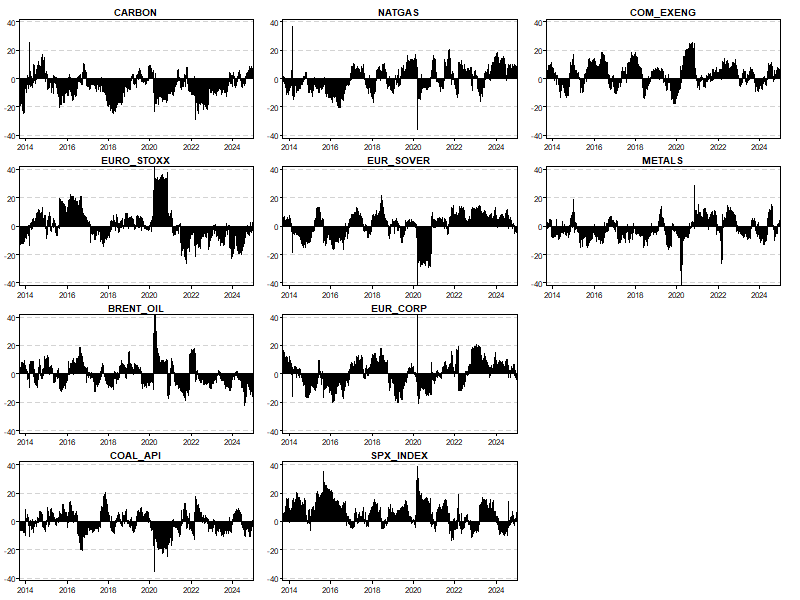
\includegraphics[width = 1.25\linewidth]{23aApdxD-12-180-RetNDC}
      \end{subfigure}
\end{figure}
\begin{figure}[H]
  \ContinuedFloat
  \centering
      \begin{subfigure}[b]{\textwidth}
        \caption{Dynamic volatility net directional connectedness}
        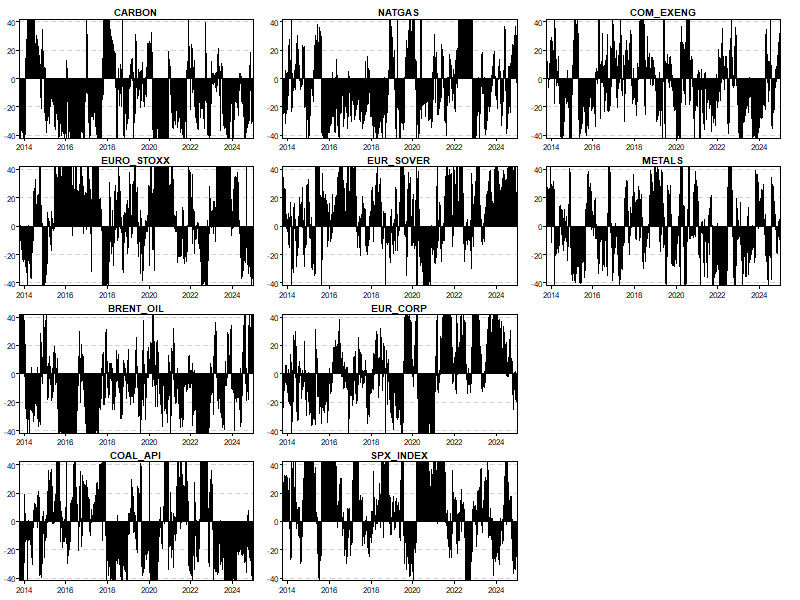
\includegraphics[width = 1.25\linewidth]{23bApdxD-12-180-VolNDC}
      \end{subfigure}
\end{figure}



\subsubsection{Static Return and Volatility Pairwise Directional Connectedness}

\begin{figure}[!ht]
  \caption{Network Representation of Pairwise Connectedness Index (Jan 2013 – Jan 2025)}
  \begin{minipage}{.8\textwidth}
    \subfloat[Static Return PCI network]{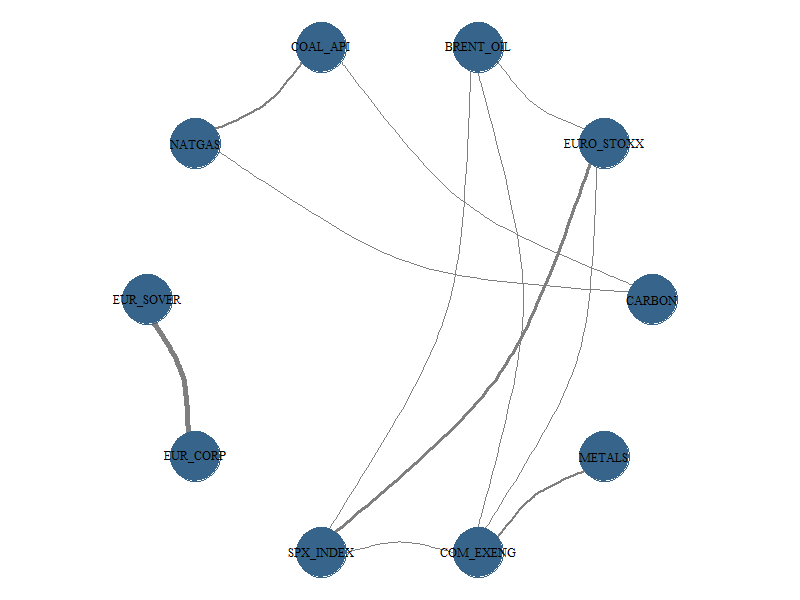
\includegraphics[width = \linewidth]{24aApdxD-12-180-RetNtwrk}}
  \end{minipage}
  \hfill
  \begin{minipage}{.8\textwidth}
    \subfloat[Static Volatility PCI network]{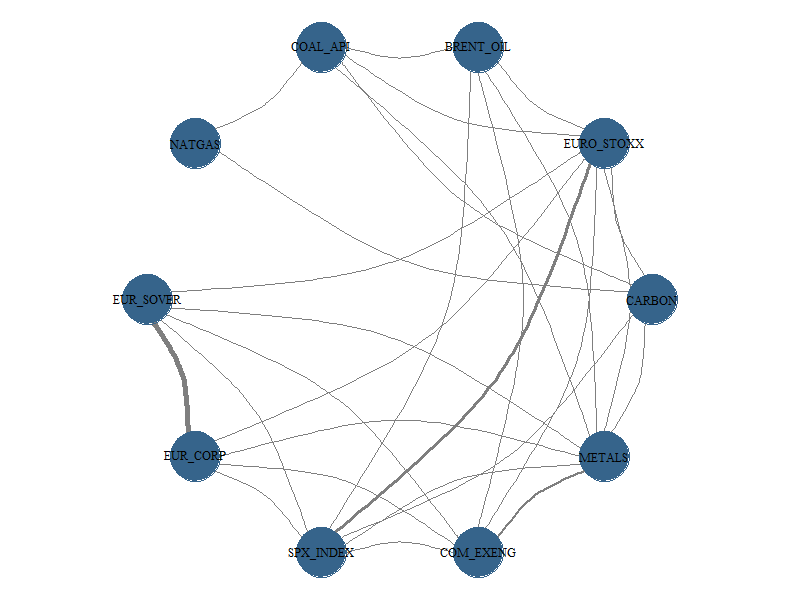
\includegraphics[width = \linewidth]{24bApdxD-12-180-VolNtwrk}}
  \end{minipage}
\end{figure}



\newpage

\subsubsection{Dynamic Return and Volatility Pairwise Directional Connectedness}

\begin{figure}[!ht]
  \caption{Dynamic Return and Volatility Pairwise Connectedness Index (Jan 2013 – Jan 2025)}
  \centering
  \begin{subfigure}[a]{\textwidth}
    \caption{Dynamic return PCI}
    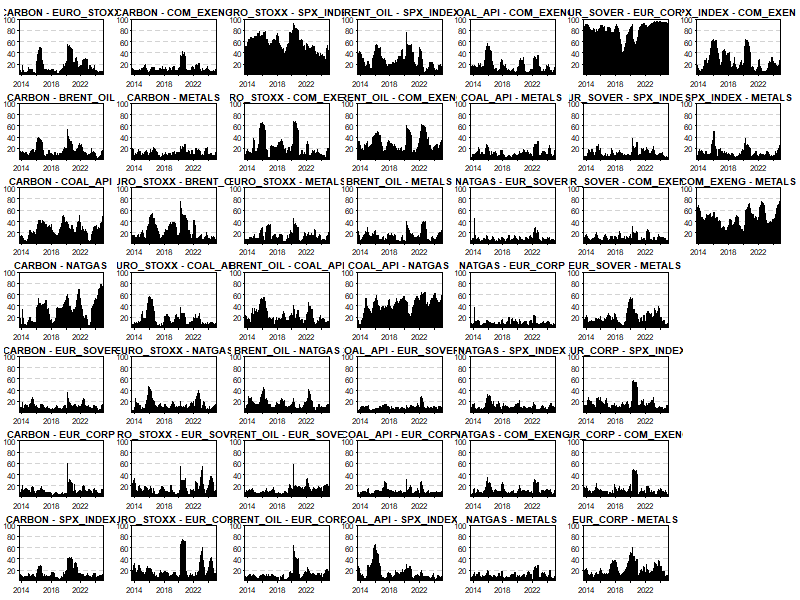
\includegraphics[width = 1.1\linewidth]{25aApdxD-12-180-RetPCI}
  \end{subfigure}
\end{figure}
\begin{figure}[!ht]
  \ContinuedFloat
  \centering
    \begin{subfigure}[b]{\textwidth}\ContinuedFloat
      \caption{Dynamic volatility PCI}
      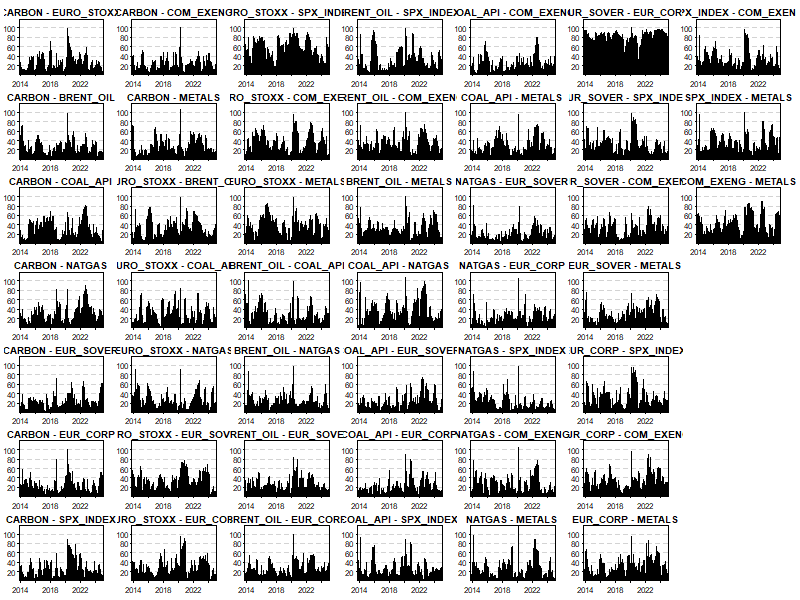
\includegraphics[width = 1.2\linewidth]{25bApdxD-12-180-VolPCI}
    \end{subfigure}
\end{figure}










\subsection{12-period forecast horizon and a rolling window of 200 observations}

\subsubsection{Static Return and Volatility Connectedness Matrix}

  \begin{table}[!ht]
    \caption{Static Return and Volatility Connectedness Matrix (Jan 2013 - Jan 2025)}
      \resizebox{\columnwidth}{!}{
      \begin{tabular}{|l|l|l|l|l|l|l|l|l|l|l|l|}
    \multicolumn{12}{@{}l}{\em(a) Carbon returns connectedness matrix}\\ \hline
        ~ & CARBON & EUROSTOXX & BRENTOIL & COALAPI & NATGAS & EURSOVER & EURCORP & SPXINDEX & COMEXENG & METALS & FROM \\ \hline
        CARBON & 59.98 & 4 & 3.81 & 7.85 & 10.21 & 2.49 & 2.28 & 3.48 & 2.77 & 3.13 & 40.02 \\ \hline
        EUROSTOXX & 3.28 & 49.71 & 5.71 & 3.34 & 3.13 & 3.05 & 3.68 & 19.85 & 5.21 & 3.03 & 50.29 \\ \hline
        BRENTOIL & 3.5 & 6.01 & 57.33 & 5.44 & 3.62 & 2.69 & 2.35 & 7.28 & 8.29 & 3.5 & 42.67 \\ \hline
        COALAPI & 6.34 & 3.78 & 5.8 & 55.96 & 13.77 & 1.86 & 2.05 & 3.84 & 3.96 & 2.64 & 44.04 \\ \hline
        NATGAS & 9.93 & 3.04 & 3.89 & 13.57 & 58.66 & 1.81 & 1.77 & 2.5 & 2.57 & 2.25 & 41.34 \\ \hline
        EURSOVER & 2.04 & 3.01 & 2.69 & 1.68 & 1.69 & 48.28 & 31.89 & 2.3 & 2.06 & 4.36 & 51.72 \\ \hline
        EURCORP & 1.98 & 5.05 & 2.72 & 1.75 & 1.82 & 30.35 & 45.45 & 3.97 & 2.55 & 4.36 & 54.55 \\ \hline
        SPXINDEX & 2.43 & 17.94 & 6.82 & 3.36 & 2.04 & 2.32 & 2.74 & 53.46 & 6.4 & 2.51 & 46.54 \\ \hline
        COMEXENG & 2.49 & 5.09 & 7.45 & 3.49 & 2.41 & 2.17 & 2.38 & 6.6 & 53.02 & 14.9 & 46.98 \\ \hline
        METALS & 2.38 & 3.18 & 3.13 & 2.29 & 2.47 & 4.84 & 5.59 & 2.98 & 16.13 & 57.02 & 42.98 \\ \hline
        DST(TO) & 34.37 & 51.09 & 42.02 & 42.78 & 41.16 & 51.58 & 54.72 & 52.79 & 49.94 & 40.68 & 461.13 \\ \hline
        Inc. Own & 94.35 & 100.8 & 99.35 & 98.74 & 99.82 & 99.86 & 100.17 & 106.25 & 102.96 & 97.69 & cTCI/TCI \\ \hline
        NS (NET) & -5.65 & 0.8 & -0.65 & -1.26 & -0.18 & -0.14 & 0.17 & 6.25 & 2.96 & -2.31 & 51.24/46.11 \\ \hline
    \end{tabular}
    }
    \bigskip
      \resizebox{\columnwidth}{!}{
    \begin{tabular}{|l|l|l|l|l|l|l|l|l|l|l|l|}
    \multicolumn{12}{@{}l}{\em(b) Carbon volatility connectedness matrix}\\ \hline
        ~ & CARBON & EUROSTOXX & BRENTOIL & COALAPI & NATGAS & EURSOVER & EURCORP & SPXINDEX & COMEXENG & METALS & FROM \\ \hline
        CARBON & 51.77 & 4.95 & 4.62 & 7.64 & 7.57 & 4.25 & 4.08 & 5.87 & 4.28 & 4.97 & 48.23 \\ \hline
        EUROSTOXX & 3.95 & 44.7 & 5.26 & 4 & 4.01 & 5.47 & 4.39 & 16.25 & 5.63 & 6.33 & 55.3 \\ \hline
        BRENTOIL & 4.33 & 6.94 & 48.98 & 5.34 & 4.07 & 4.39 & 5.01 & 6.77 & 7.45 & 6.73 & 51.02 \\ \hline
        COALAPI & 5.18 & 6.48 & 4.42 & 54.18 & 8.27 & 4.19 & 3.09 & 5.01 & 3.51 & 5.67 & 45.82 \\ \hline
        NATGAS & 4.87 & 5.04 & 3.94 & 8.7 & 55.58 & 4.08 & 4.28 & 5.31 & 3.85 & 4.35 & 44.42 \\ \hline
        EURSOVER & 2.39 & 6.61 & 3.52 & 2.68 & 2.03 & 43.31 & 24.59 & 5.95 & 4.24 & 4.68 & 56.69 \\ \hline
        EURCORP & 3.04 & 6.01 & 2.75 & 2.55 & 2.71 & 27.87 & 40.08 & 6.26 & 5.14 & 3.58 & 59.92 \\ \hline
        SPXINDEX & 3.75 & 15.2 & 5.1 & 3.55 & 2.01 & 5.11 & 4.18 & 50.28 & 4.96 & 5.87 & 49.72 \\ \hline
        COMEXENG & 2.95 & 8.09 & 4.83 & 4.12 & 4.36 & 5.67 & 5.7 & 7.07 & 47.39 & 9.81 & 52.61 \\ \hline
        METALS & 4.08 & 8.78 & 4.77 & 4.27 & 4.3 & 5.29 & 6.67 & 6.72 & 10.22 & 44.9 & 55.1 \\ \hline
        DST(TO) & 34.53 & 68.1 & 39.22 & 42.85 & 39.32 & 66.32 & 61.99 & 65.21 & 49.29 & 51.99 & 518.82 \\ \hline
        Inc. Own & 86.3 & 112.8 & 88.19 & 97.03 & 94.9 & 109.63 & 102.07 & 115.49 & 96.68 & 96.89 & cTCI/TCI \\ \hline
        NS (NET) & -13.7 & 12.8 & -11.81 & -2.97 & -5.1 & 9.63 & 2.07 & 15.49 & -3.32 & -3.11 & 57.65/51.88 \\ \hline
    \end{tabular}
    }
\end{table}




\subsubsection{Dynamic Return and Volatility Net Directional Connectedness}

\begin{figure}[H]
  \caption{Dynamic Net Directional Connectedness (Jan 2013 – Jan 2025)}
    \centering
      \begin{subfigure}[a]{\textwidth}
        \caption{Dynamic return net directional connectedness}
        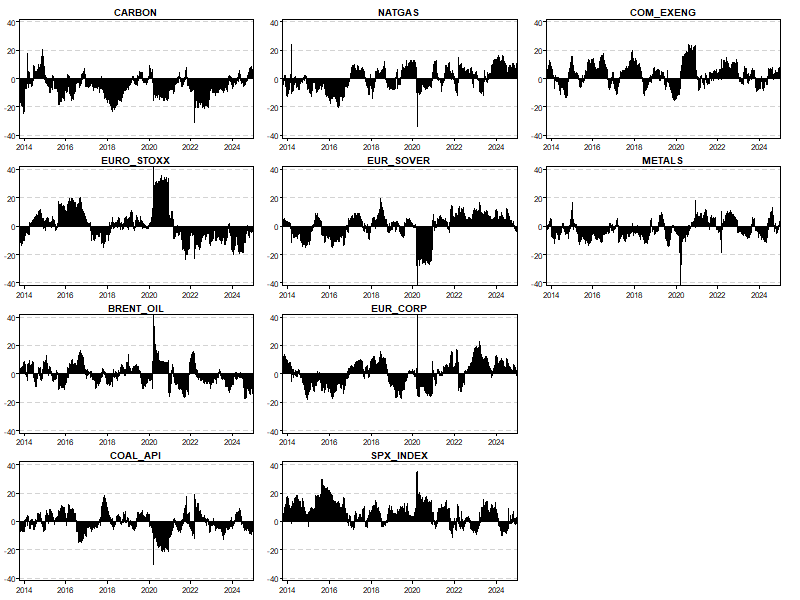
\includegraphics[width = 1.25\linewidth]{26aApdxD-12-200-RetNDC}
      \end{subfigure}
\end{figure}
\begin{figure}[H]
  \ContinuedFloat
  \centering
      \begin{subfigure}[b]{\textwidth}
        \caption{Dynamic volatility net directional connectedness}
        \includegraphics[width = 1.25\linewidth]{26bApdxD-12-200-VolNDC}
      \end{subfigure}
\end{figure}



\subsubsection{Static Return and Volatility Pairwise Directional Connectedness}

\begin{figure}[!ht]
  \caption{Network Representation of Pairwise Connectedness Index (Jan 2013 – Jan 2025)}
  \begin{minipage}{.8\textwidth}
    \subfloat[Static Return PCI network]{\includegraphics[width = \linewidth]{27aApdxD-12-200-RetNtwrk}}
  \end{minipage}
  \hfill
  \begin{minipage}{.8\textwidth}
    \subfloat[Static Volatility PCI network]{\includegraphics[width = \linewidth]{27bApdxD-12-200-VolNtwrk}}
  \end{minipage}
\end{figure}



\newpage

\subsubsection{Dynamic Return and Volatility Pairwise Directional Connectedness}

\begin{figure}[!ht]
  \caption{Dynamic Return and Volatility Pairwise Connectedness Index (Jan 2013 – Jan 2025)}
  \centering
  \begin{subfigure}[a]{\textwidth}
    \caption{Dynamic return PCI}
    \includegraphics[width = 1.1\linewidth]{28aApdxD-12-200-RetPCI}
  \end{subfigure}
\end{figure}
\begin{figure}[!ht]
  \ContinuedFloat
  \centering
    \begin{subfigure}[b]{\textwidth}\ContinuedFloat
      \caption{Dynamic volatility PCI}
      \includegraphics[width = 1.2\linewidth]{28bApdxD-12-200-VolPCI}
    \end{subfigure}
\end{figure}












\subsection{12-period forecast horizon and a rolling window of 220 observations}

\subsubsection{Static Return and Volatility Connectedness Matrix}

  \begin{table}[!ht]
    \caption{Static Return and Volatility Connectedness Matrix (Jan 2013 - Jan 2025)}
      \resizebox{\columnwidth}{!}{
      \begin{tabular}{|l|l|l|l|l|l|l|l|l|l|l|l|}
    \multicolumn{12}{@{}l}{\em(a) Carbon returns connectedness matrix}\\ \hline
        ~ & CARBON & EUROSTOXX & BRENTOIL & COALAPI & NATGAS & EURSOVER & EURCORP & SPXINDEX & COMEXENG & METALS & FROM \\ \hline
        CARBON & 61.29 & 3.94 & 3.67 & 7.78 & 10.07 & 2.3 & 2.13 & 3.29 & 2.61 & 2.93 & 38.71 \\ \hline
        EUROSTOXX & 3.18 & 50.75 & 5.67 & 3.23 & 2.95 & 2.75 & 3.44 & 20.11 & 5.14 & 2.78 & 49.25 \\ \hline
        BRENTOIL & 3.31 & 5.92 & 58.37 & 5.39 & 3.49 & 2.52 & 2.23 & 7.2 & 8.31 & 3.26 & 41.63 \\ \hline
        COALAPI & 6.22 & 3.66 & 5.74 & 56.99 & 13.87 & 1.72 & 1.89 & 3.7 & 3.83 & 2.39 & 43.01 \\ \hline
        NATGAS & 9.79 & 2.87 & 3.75 & 13.75 & 59.92 & 1.63 & 1.61 & 2.24 & 2.38 & 2.06 & 40.08 \\ \hline
        EURSOVER & 1.87 & 2.8 & 2.48 & 1.5 & 1.48 & 49.27 & 32.33 & 2.16 & 1.85 & 4.26 & 50.73 \\ \hline
        EURCORP & 1.84 & 5 & 2.61 & 1.57 & 1.62 & 30.67 & 46.12 & 3.92 & 2.43 & 4.23 & 53.88 \\ \hline
        SPXINDEX & 2.26 & 18.11 & 6.71 & 3.22 & 1.81 & 2.14 & 2.59 & 54.44 & 6.44 & 2.29 & 45.56 \\ \hline
        COMEXENG & 2.33 & 5.03 & 7.43 & 3.35 & 2.18 & 1.97 & 2.22 & 6.63 & 53.89 & 14.98 & 46.11 \\ \hline
        METALS & 2.22 & 2.93 & 2.91 & 2.08 & 2.25 & 4.77 & 5.51 & 2.77 & 16.29 & 58.28 & 41.72 \\ \hline
        DST(TO) & 33.01 & 50.26 & 40.96 & 41.87 & 39.71 & 50.46 & 53.95 & 52 & 49.28 & 39.18 & 450.7 \\ \hline
        Inc. Own & 94.3 & 101.01 & 99.33 & 98.86 & 99.62 & 99.73 & 100.06 & 106.44 & 103.17 & 97.47 & cTCI/TCI \\ \hline
        NS (NET) & -5.7 & 1.01 & -0.67 & -1.14 & -0.38 & -0.27 & 0.06 & 6.44 & 3.17 & -2.53 & 50.08/45.07 \\ \hline
    \end{tabular}
    }
    \bigskip
      \resizebox{\columnwidth}{!}{
    \begin{tabular}{|l|l|l|l|l|l|l|l|l|l|l|l|}
    \multicolumn{12}{@{}l}{\em(b) Carbon volatility connectedness matrix}\\ \hline
        ~ & CARBON & EUROSTOXX & BRENTOIL & COALAPI & NATGAS & EURSOVER & EURCORP & SPXINDEX & COMEXENG & METALS & FROM \\ \hline
        CARBON & 53.98 & 4.97 & 4.32 & 7.64 & 7.18 & 3.84 & 3.72 & 5.49 & 4.29 & 4.56 & 46.02 \\ \hline
        EUROSTOXX & 3.55 & 46.21 & 4.99 & 3.61 & 3.61 & 5.32 & 4.27 & 16.81 & 5.63 & 6.01 & 53.79 \\ \hline
        BRENTOIL & 3.82 & 6.9 & 51.01 & 5.18 & 3.86 & 3.98 & 4.53 & 6.63 & 7.62 & 6.47 & 48.99 \\ \hline
        COALAPI & 5.06 & 5.98 & 3.68 & 57.01 & 7.87 & 3.96 & 2.92 & 4.6 & 3.39 & 5.53 & 42.99 \\ \hline
        NATGAS & 4.63 & 4.71 & 3.52 & 8.47 & 58.3 & 3.77 & 4.15 & 4.94 & 3.53 & 3.99 & 41.7 \\ \hline
        EURSOVER & 2.06 & 6.39 & 3.31 & 2.32 & 1.72 & 44.95 & 25.12 & 5.85 & 3.77 & 4.53 & 55.05 \\ \hline
        EURCORP & 2.67 & 6.01 & 2.68 & 2.1 & 2.2 & 28.56 & 41.62 & 6.19 & 4.53 & 3.42 & 58.38 \\ \hline
        SPXINDEX & 3.46 & 15.35 & 4.67 & 3.27 & 1.77 & 4.68 & 3.85 & 52.71 & 4.66 & 5.58 & 47.29 \\ \hline
        COMEXENG & 2.45 & 8.05 & 4.81 & 3.83 & 3.94 & 5.14 & 5.21 & 6.79 & 49.88 & 9.9 & 50.12 \\ \hline
        METALS & 3.87 & 8.67 & 4.35 & 4 & 3.91 & 5.1 & 6.19 & 6.11 & 10.51 & 47.28 & 52.72 \\ \hline
        DST(TO) & 31.56 & 67.03 & 36.35 & 40.42 & 36.07 & 64.35 & 59.96 & 63.39 & 47.93 & 49.97 & 497.04 \\ \hline
        Inc. Own & 85.54 & 113.25 & 87.36 & 97.43 & 94.38 & 109.3 & 101.59 & 116.09 & 97.81 & 97.25 & cTCI/TCI \\ \hline
        NS (NET) & -14.46 & 13.25 & -12.64 & -2.57 & -5.62 & 9.3 & 1.59 & 16.09 & -2.19 & -2.75 & 55.23/49.70 \\ \hline
    \end{tabular}
    }
\end{table}




\subsubsection{Dynamic Return and Volatility Net Directional Connectedness}

\begin{figure}[H]
  \caption{Dynamic Net Directional Connectedness (Jan 2013 – Jan 2025)}
    \centering
      \begin{subfigure}[a]{\textwidth}
        \caption{Dynamic return net directional connectedness}
        \includegraphics[width = 1.25\linewidth]{29aApdxD-12-220-RetNDC}
      \end{subfigure}
\end{figure}
\begin{figure}[H]
  \ContinuedFloat
  \centering
      \begin{subfigure}[b]{\textwidth}
        \caption{Dynamic volatility net directional connectedness}
        \includegraphics[width = 1.25\linewidth]{29bApdxD-12-220-VolNDC}
      \end{subfigure}
\end{figure}



\subsubsection{Static Return and Volatility Pairwise Directional Connectedness}

\begin{figure}[!ht]
  \caption{Network Representation of Pairwise Connectedness Index (Jan 2013 – Jan 2025)}
  \begin{minipage}{.8\textwidth}
    \subfloat[Static Return PCI network]{\includegraphics[width = \linewidth]{30aApdxD-12-220-RetNtwrk}}
  \end{minipage}
  \hfill
  \begin{minipage}{.8\textwidth}
    \subfloat[Static Volatility PCI network]{\includegraphics[width = \linewidth]{30bApdxD-12-220-VolNtwrk}}
  \end{minipage}
\end{figure}



\newpage

\subsubsection{Dynamic Return and Volatility Pairwise Directional Connectedness}

\begin{figure}[!ht]
  \caption{Dynamic Return and Volatility Pairwise Connectedness Index (Jan 2013 – Jan 2025)}
  \centering
  \begin{subfigure}[a]{\textwidth}
    \caption{Dynamic return PCI}
    \includegraphics[width = 1.1\linewidth]{31aApdxD-12-220-RetPCI}
  \end{subfigure}
\end{figure}
\begin{figure}[!ht]
  \ContinuedFloat
  \centering
    \begin{subfigure}[b]{\textwidth}\ContinuedFloat
      \caption{Dynamic volatility PCI}
      \includegraphics[width = 1.2\linewidth]{31bApdxD-12-220-VolPCI}
    \end{subfigure}
\end{figure}










\end{landscape}

\newpage

\renewcommand\refname{References}
\bibliography{EUAbibliography.bib}


\end{document}
